\documentclass[twoside]{book}

% Packages required by doxygen
\usepackage{fixltx2e}
\usepackage{calc}
\usepackage{doxygen}
\usepackage[export]{adjustbox} % also loads graphicx
\usepackage{graphicx}
\usepackage[utf8]{inputenc}
\usepackage{makeidx}
\usepackage{multicol}
\usepackage{multirow}
\PassOptionsToPackage{warn}{textcomp}
\usepackage{textcomp}
\usepackage[nointegrals]{wasysym}
\usepackage[table]{xcolor}

% Font selection
\usepackage[T1]{fontenc}
\usepackage[scaled=.90]{helvet}
\usepackage{courier}
\usepackage{amssymb}
\usepackage{sectsty}
\renewcommand{\familydefault}{\sfdefault}
\allsectionsfont{%
  \fontseries{bc}\selectfont%
  \color{darkgray}%
}
\renewcommand{\DoxyLabelFont}{%
  \fontseries{bc}\selectfont%
  \color{darkgray}%
}
\newcommand{\+}{\discretionary{\mbox{\scriptsize$\hookleftarrow$}}{}{}}

% Page & text layout
\usepackage{geometry}
\geometry{%
  a4paper,%
  top=2.5cm,%
  bottom=2.5cm,%
  left=2.5cm,%
  right=2.5cm%
}
\tolerance=750
\hfuzz=15pt
\hbadness=750
\setlength{\emergencystretch}{15pt}
\setlength{\parindent}{0cm}
\setlength{\parskip}{3ex plus 2ex minus 2ex}
\makeatletter
\renewcommand{\paragraph}{%
  \@startsection{paragraph}{4}{0ex}{-1.0ex}{1.0ex}{%
    \normalfont\normalsize\bfseries\SS@parafont%
  }%
}
\renewcommand{\subparagraph}{%
  \@startsection{subparagraph}{5}{0ex}{-1.0ex}{1.0ex}{%
    \normalfont\normalsize\bfseries\SS@subparafont%
  }%
}
\makeatother

% Headers & footers
\usepackage{fancyhdr}
\pagestyle{fancyplain}
\fancyhead[LE]{\fancyplain{}{\bfseries\thepage}}
\fancyhead[CE]{\fancyplain{}{}}
\fancyhead[RE]{\fancyplain{}{\bfseries\leftmark}}
\fancyhead[LO]{\fancyplain{}{\bfseries\rightmark}}
\fancyhead[CO]{\fancyplain{}{}}
\fancyhead[RO]{\fancyplain{}{\bfseries\thepage}}
\fancyfoot[LE]{\fancyplain{}{}}
\fancyfoot[CE]{\fancyplain{}{}}
\fancyfoot[RE]{\fancyplain{}{\bfseries\scriptsize Generated by Doxygen }}
\fancyfoot[LO]{\fancyplain{}{\bfseries\scriptsize Generated by Doxygen }}
\fancyfoot[CO]{\fancyplain{}{}}
\fancyfoot[RO]{\fancyplain{}{}}
\renewcommand{\footrulewidth}{0.4pt}
\renewcommand{\chaptermark}[1]{%
  \markboth{#1}{}%
}
\renewcommand{\sectionmark}[1]{%
  \markright{\thesection\ #1}%
}

% Indices & bibliography
\usepackage{natbib}
\usepackage[titles]{tocloft}
\setcounter{tocdepth}{3}
\setcounter{secnumdepth}{5}
\makeindex

% Hyperlinks (required, but should be loaded last)
\usepackage{ifpdf}
\ifpdf
  \usepackage[pdftex,pagebackref=true]{hyperref}
\else
  \usepackage[ps2pdf,pagebackref=true]{hyperref}
\fi
\hypersetup{%
  colorlinks=true,%
  linkcolor=blue,%
  citecolor=blue,%
  unicode%
}

% Custom commands
\newcommand{\clearemptydoublepage}{%
  \newpage{\pagestyle{empty}\cleardoublepage}%
}

\usepackage{caption}
\captionsetup{labelsep=space,justification=centering,font={bf},singlelinecheck=off,skip=4pt,position=top}

%===== C O N T E N T S =====

\begin{document}

% Titlepage & ToC
\hypersetup{pageanchor=false,
             bookmarksnumbered=true,
             pdfencoding=unicode
            }
\pagenumbering{alph}
\begin{titlepage}
\vspace*{7cm}
\begin{center}%
{\Large L\+A\+R\+\_\+1\+\_\+0 \\[1ex]\large 001 }\\
\vspace*{1cm}
{\large Generated by Doxygen 1.8.14}\\
\end{center}
\end{titlepage}
\clearemptydoublepage
\pagenumbering{roman}
\tableofcontents
\clearemptydoublepage
\pagenumbering{arabic}
\hypersetup{pageanchor=true}

%--- Begin generated contents ---
\chapter{Laboratory of Applied Robotics Documentation}
\label{index}\hypertarget{index}{}Authors\+: ~\newline
Riccardo Franceschini, Marvin Mouroum ~\newline
 \hypertarget{index_Robotic-Mapping}{}\section{Robotic-\/\+Mapping}\label{index_Robotic-Mapping}
The robotic mapping process is presented in the following slides. All relevant classes and methods will be shown and the theoretic aspects will be visualized. ~\newline
                   \hypertarget{index_Path-Planning}{}\section{Path-\/\+Planning}\label{index_Path-Planning}
etc... 
\chapter{Namespace Index}
\section{Namespace List}
Here is a list of all documented namespaces with brief descriptions\+:\begin{DoxyCompactList}
\item\contentsline{section}{\mbox{\hyperlink{namespace_geometry2_d}{Geometry2D}} \\*Geometries, such as Pentagons, Circles and other 2D Shapes }{\pageref{namespace_geometry2_d}}{}
\item\contentsline{section}{\mbox{\hyperlink{namespace_image_processing}{Image\+Processing}} \\*Transforming, classifying and creating images }{\pageref{namespace_image_processing}}{}
\item\contentsline{section}{\mbox{\hyperlink{namespace_l_a_r}{L\+AR}} \\*Objects that are specific for the Laboratory of Applied Robotics Projects }{\pageref{namespace_l_a_r}}{}
\item\contentsline{section}{\mbox{\hyperlink{namespace_path2_d}{Path2D}} \\*Contains Datatypes for planning and constructing 2D paths }{\pageref{namespace_path2_d}}{}
\item\contentsline{section}{\mbox{\hyperlink{namespace_path2_d_1_1_element}{Path2\+D\+::\+Element}} \\*Contains basic elements needed for describing a path }{\pageref{namespace_path2_d_1_1_element}}{}
\end{DoxyCompactList}

\chapter{Hierarchical Index}
\section{Class Hierarchy}
This inheritance list is sorted roughly, but not completely, alphabetically\+:\begin{DoxyCompactList}
\item \contentsline{section}{Calibration\+\_\+\+Instrinsic}{\pageref{class_calibration___instrinsic}}{}
\item \contentsline{section}{Cell}{\pageref{class_cell}}{}
\item \contentsline{section}{Character\+\_\+\+Recognition\+\_\+\+Algorithm}{\pageref{class_character___recognition___algorithm}}{}
\begin{DoxyCompactList}
\item \contentsline{section}{Optical\+\_\+\+Character\+\_\+\+Recognition}{\pageref{class_optical___character___recognition}}{}
\item \contentsline{section}{Template\+\_\+\+Character\+\_\+\+Recognition}{\pageref{class_template___character___recognition}}{}
\end{DoxyCompactList}
\item \contentsline{section}{Clipper}{\pageref{class_clipper}}{}
\item \contentsline{section}{Path\+Finder\+:\+:Collision\+Detector}{\pageref{class_path_finder_1_1_collision_detector}}{}
\item \contentsline{section}{Color\+\_\+\+Processing}{\pageref{class_color___processing}}{}
\item \contentsline{section}{Digit\+\_\+\+Recognition}{\pageref{class_digit___recognition}}{}
\item \contentsline{section}{Digit\+Result\+Distribution}{\pageref{struct_digit_result_distribution}}{}
\item \contentsline{section}{H\+S\+V\+Filter\+Range}{\pageref{struct_h_s_v_filter_range}}{}
\item \contentsline{section}{Inverse\+\_\+\+Perspective\+\_\+\+Mapping}{\pageref{class_inverse___perspective___mapping}}{}
\item \contentsline{section}{Line}{\pageref{class_line}}{}
\begin{DoxyCompactList}
\item \contentsline{section}{Circular\+Line}{\pageref{class_circular_line}}{}
\item \contentsline{section}{Straight\+Line}{\pageref{class_straight_line}}{}
\end{DoxyCompactList}
\item \contentsline{section}{Map}{\pageref{class_map}}{}
\item \contentsline{section}{Path}{\pageref{class_path}}{}
\item \contentsline{section}{Path\+Coordinates}{\pageref{class_path_coordinates}}{}
\item \contentsline{section}{Path\+Finder}{\pageref{class_path_finder}}{}
\begin{DoxyCompactList}
\item \contentsline{section}{Dubin\+Path\+Finder}{\pageref{class_dubin_path_finder}}{}
\end{DoxyCompactList}
\item \contentsline{section}{People\+Storage}{\pageref{struct_people_storage}}{}
\item \contentsline{section}{Position}{\pageref{class_position}}{}
\item \contentsline{section}{Dubin\+Path\+Finder\+:\+:Possible\+Dubin\+Path}{\pageref{class_dubin_path_finder_1_1_possible_dubin_path}}{}
\item \contentsline{section}{Settings}{\pageref{class_settings}}{}
\item \contentsline{section}{Shape}{\pageref{class_shape}}{}
\begin{DoxyCompactList}
\item \contentsline{section}{Circle}{\pageref{class_circle}}{}
\begin{DoxyCompactList}
\item \contentsline{section}{People}{\pageref{class_people}}{}
\item \contentsline{section}{Robot}{\pageref{class_robot}}{}
\end{DoxyCompactList}
\item \contentsline{section}{Obstacle}{\pageref{class_obstacle}}{}
\item \contentsline{section}{Polygon}{\pageref{class_polygon}}{}
\begin{DoxyCompactList}
\item \contentsline{section}{Hexagon}{\pageref{class_hexagon}}{}
\item \contentsline{section}{Pentagon}{\pageref{class_pentagon}}{}
\item \contentsline{section}{Rectangle}{\pageref{class_rectangle}}{}
\begin{DoxyCompactList}
\item \contentsline{section}{Arena}{\pageref{class_arena}}{}
\item \contentsline{section}{Exit\+Point}{\pageref{class_exit_point}}{}
\item \contentsline{section}{Square}{\pageref{class_square}}{}
\end{DoxyCompactList}
\item \contentsline{section}{Triangle}{\pageref{class_triangle}}{}
\end{DoxyCompactList}
\end{DoxyCompactList}
\item \contentsline{section}{standard\+Conf}{\pageref{structstandard_conf}}{}
\item \contentsline{section}{Undistorsion}{\pageref{class_undistorsion}}{}
\end{DoxyCompactList}

\chapter{Class Index}
\section{Class List}
Here are the classes, structs, unions and interfaces with brief descriptions\+:\begin{DoxyCompactList}
\item\contentsline{section}{\mbox{\hyperlink{class_arena}{Arena}} }{\pageref{class_arena}}{}
\item\contentsline{section}{\mbox{\hyperlink{class_calibration___instrinsic}{Calibration\+\_\+\+Instrinsic}} }{\pageref{class_calibration___instrinsic}}{}
\item\contentsline{section}{\mbox{\hyperlink{class_cell}{Cell}} }{\pageref{class_cell}}{}
\item\contentsline{section}{\mbox{\hyperlink{class_character___recognition___algorithm}{Character\+\_\+\+Recognition\+\_\+\+Algorithm}} \\*Abstract class for character recognition algorithms }{\pageref{class_character___recognition___algorithm}}{}
\item\contentsline{section}{\mbox{\hyperlink{class_circle}{Circle}} }{\pageref{class_circle}}{}
\item\contentsline{section}{\mbox{\hyperlink{class_color___processing}{Color\+\_\+\+Processing}} }{\pageref{class_color___processing}}{}
\item\contentsline{section}{\mbox{\hyperlink{class_digit___recognition}{Digit\+\_\+\+Recognition}} \\*Used to detect digits in the arena and export \mbox{\hyperlink{struct_people_data}{People\+Data}} }{\pageref{class_digit___recognition}}{}
\item\contentsline{section}{\mbox{\hyperlink{struct_digit_result_distribution}{Digit\+Result\+Distribution}} }{\pageref{struct_digit_result_distribution}}{}
\item\contentsline{section}{\mbox{\hyperlink{class_exit_point}{Exit\+Point}} }{\pageref{class_exit_point}}{}
\item\contentsline{section}{\mbox{\hyperlink{class_hexagon}{Hexagon}} }{\pageref{class_hexagon}}{}
\item\contentsline{section}{\mbox{\hyperlink{struct_h_s_v_filter_range}{H\+S\+V\+Filter\+Range}} }{\pageref{struct_h_s_v_filter_range}}{}
\item\contentsline{section}{\mbox{\hyperlink{class_image___processing}{Image\+\_\+\+Processing}} }{\pageref{class_image___processing}}{}
\item\contentsline{section}{\mbox{\hyperlink{class_inverse___perspective___mapping}{Inverse\+\_\+\+Perspective\+\_\+\+Mapping}} }{\pageref{class_inverse___perspective___mapping}}{}
\item\contentsline{section}{\mbox{\hyperlink{class_map}{Map}} }{\pageref{class_map}}{}
\item\contentsline{section}{\mbox{\hyperlink{class_obstacle}{Obstacle}} }{\pageref{class_obstacle}}{}
\item\contentsline{section}{\mbox{\hyperlink{class_optical___character___recognition}{Optical\+\_\+\+Character\+\_\+\+Recognition}} \\*O\+CP algorithm from tesseract library }{\pageref{class_optical___character___recognition}}{}
\item\contentsline{section}{\mbox{\hyperlink{class_pentagon}{Pentagon}} }{\pageref{class_pentagon}}{}
\item\contentsline{section}{\mbox{\hyperlink{class_people}{People}} }{\pageref{class_people}}{}
\item\contentsline{section}{\mbox{\hyperlink{struct_people_data}{People\+Data}} \\*Data object that is beeing used to build a \mbox{\hyperlink{class_people}{People}} Object for the map representation }{\pageref{struct_people_data}}{}
\item\contentsline{section}{\mbox{\hyperlink{class_settings}{Settings}} }{\pageref{class_settings}}{}
\item\contentsline{section}{\mbox{\hyperlink{class_shape}{Shape}} }{\pageref{class_shape}}{}
\item\contentsline{section}{\mbox{\hyperlink{class_square}{Square}} }{\pageref{class_square}}{}
\item\contentsline{section}{\mbox{\hyperlink{class_template___character___recognition}{Template\+\_\+\+Character\+\_\+\+Recognition}} }{\pageref{class_template___character___recognition}}{}
\item\contentsline{section}{\mbox{\hyperlink{class_triangle}{Triangle}} }{\pageref{class_triangle}}{}
\item\contentsline{section}{\mbox{\hyperlink{class_undistorsion}{Undistorsion}} }{\pageref{class_undistorsion}}{}
\item\contentsline{section}{\mbox{\hyperlink{struct_user_data}{User\+Data}} }{\pageref{struct_user_data}}{}
\end{DoxyCompactList}

\chapter{Namespace Documentation}
\hypertarget{namespace_geometry2_d}{}\section{Geometry2D Namespace Reference}
\label{namespace_geometry2_d}\index{Geometry2D@{Geometry2D}}


contains Geometries, such as Pentagons, Circles and other 2D Shapes  


\subsection*{Classes}
\begin{DoxyCompactItemize}
\item 
class \mbox{\hyperlink{class_geometry2_d_1_1_circle}{Circle}}
\begin{DoxyCompactList}\small\item\em \mbox{\hyperlink{class_geometry2_d_1_1_circle}{Circle}} class is able to detect and save the arena given a photo. \end{DoxyCompactList}\item 
class \mbox{\hyperlink{class_geometry2_d_1_1_hexagon}{Hexagon}}
\begin{DoxyCompactList}\small\item\em Class for handling hexagon obstacles. \end{DoxyCompactList}\item 
class \mbox{\hyperlink{class_geometry2_d_1_1_pentagon}{Pentagon}}
\begin{DoxyCompactList}\small\item\em Class for hadling pentagon obstacles in the map. \end{DoxyCompactList}\item 
class \mbox{\hyperlink{class_geometry2_d_1_1_polygon}{Polygon}}
\item 
class \mbox{\hyperlink{class_geometry2_d_1_1_rectangle}{Rectangle}}
\begin{DoxyCompactList}\small\item\em Class for handling square in the map. \end{DoxyCompactList}\item 
class \mbox{\hyperlink{class_geometry2_d_1_1_shape}{Shape}}
\begin{DoxyCompactList}\small\item\em class for handling all the shapes in the map \end{DoxyCompactList}\item 
class \mbox{\hyperlink{class_geometry2_d_1_1_square}{Square}}
\begin{DoxyCompactList}\small\item\em A \mbox{\hyperlink{class_geometry2_d_1_1_shape}{Shape}} type similar to a \mbox{\hyperlink{class_geometry2_d_1_1_rectangle}{Rectangle}} but with equdistant lengths. \end{DoxyCompactList}\item 
class \mbox{\hyperlink{class_geometry2_d_1_1_triangle}{Triangle}}
\begin{DoxyCompactList}\small\item\em class for handling triangle obstacles \end{DoxyCompactList}\end{DoxyCompactItemize}


\subsection{Detailed Description}
contains Geometries, such as Pentagons, Circles and other 2D Shapes 
\hypertarget{namespace_image_processing}{}\section{Image\+Processing Namespace Reference}
\label{namespace_image_processing}\index{Image\+Processing@{Image\+Processing}}


transforming, classifying and creating images  


\subsection*{Classes}
\begin{DoxyCompactItemize}
\item 
class \mbox{\hyperlink{class_image_processing_1_1_calibration___instrinsic}{Calibration\+\_\+\+Instrinsic}}
\begin{DoxyCompactList}\small\item\em function that helps calibrating the camera resulting in an undistortion matrix \end{DoxyCompactList}\item 
class \mbox{\hyperlink{class_image_processing_1_1_character___recognition___algorithm}{Character\+\_\+\+Recognition\+\_\+\+Algorithm}}
\begin{DoxyCompactList}\small\item\em abstract class for character recognition algorithms \end{DoxyCompactList}\item 
class \mbox{\hyperlink{class_image_processing_1_1_clipper}{Clipper}}
\item 
class \mbox{\hyperlink{class_image_processing_1_1_color___processing}{Color\+\_\+\+Processing}}
\begin{DoxyCompactList}\small\item\em A class that helps to extract information about the color values of pixels in an image. \end{DoxyCompactList}\item 
class \mbox{\hyperlink{class_image_processing_1_1_digit___recognition}{Digit\+\_\+\+Recognition}}
\begin{DoxyCompactList}\small\item\em The \mbox{\hyperlink{class_image_processing_1_1_digit___recognition}{Digit\+\_\+\+Recognition}} class is used to detect digits in the arena and export \mbox{\hyperlink{class_people}{People}} objects. \end{DoxyCompactList}\item 
struct \mbox{\hyperlink{struct_image_processing_1_1_digit_result_distribution}{Digit\+Result\+Distribution}}
\begin{DoxyCompactList}\small\item\em A structure that builds a distribution of digits based on their amount. \end{DoxyCompactList}\item 
struct \mbox{\hyperlink{struct_image_processing_1_1_h_s_v_filter_range}{H\+S\+V\+Filter\+Range}}
\begin{DoxyCompactList}\small\item\em A structure that helps creating a color filter. \end{DoxyCompactList}\item 
class \mbox{\hyperlink{class_image_processing_1_1_inverse___perspective___mapping}{Inverse\+\_\+\+Perspective\+\_\+\+Mapping}}
\begin{DoxyCompactList}\small\item\em produce a perspective transformation around the arena given a photo \end{DoxyCompactList}\item 
class \mbox{\hyperlink{class_image_processing_1_1_optical___character___recognition}{Optical\+\_\+\+Character\+\_\+\+Recognition}}
\begin{DoxyCompactList}\small\item\em O\+CP algorithm from tesseract library. \end{DoxyCompactList}\item 
class \mbox{\hyperlink{class_image_processing_1_1_template___character___recognition}{Template\+\_\+\+Character\+\_\+\+Recognition}}
\begin{DoxyCompactList}\small\item\em Class that performs the Template Matching Method to identify characters. \end{DoxyCompactList}\item 
class \mbox{\hyperlink{class_image_processing_1_1_undistorsion}{Undistorsion}}
\begin{DoxyCompactList}\small\item\em class for undistorsion of the images \end{DoxyCompactList}\end{DoxyCompactItemize}
\subsection*{Enumerations}
\begin{DoxyCompactItemize}
\item 
\mbox{\Hypertarget{namespace_image_processing_ac44aa6095f14cd8f892fe802e71c228b}\label{namespace_image_processing_ac44aa6095f14cd8f892fe802e71c228b}} 
enum \{ {\bfseries D\+E\+T\+E\+C\+T\+I\+ON} = 0, 
{\bfseries C\+A\+P\+T\+U\+R\+I\+NG} = 1, 
{\bfseries C\+A\+L\+I\+B\+R\+A\+T\+ED} = 2
 \}
\item 
\mbox{\Hypertarget{namespace_image_processing_afe66b5cb462eb22dcf108308418c09eb}\label{namespace_image_processing_afe66b5cb462eb22dcf108308418c09eb}} 
enum \mbox{\hyperlink{namespace_image_processing_afe66b5cb462eb22dcf108308418c09eb}{Digit\+Recognition\+Algo}} \{ {\bfseries template\+Matching}, 
{\bfseries tesseract\+O\+CP}
 \}
\begin{DoxyCompactList}\small\item\em different algorithms for recognizing digits \end{DoxyCompactList}\end{DoxyCompactItemize}
\subsection*{Functions}
\begin{DoxyCompactItemize}
\item 
\mbox{\Hypertarget{namespace_image_processing_a87e697d0a25a31287e73dc3e3a3cfe66}\label{namespace_image_processing_a87e697d0a25a31287e73dc3e3a3cfe66}} 
{\footnotesize template$<$typename T $>$ }\\int {\bfseries find\+In\+Vector} (const std\+::vector$<$ T $>$ \&vec\+Of\+Elements, const T \&element)
\end{DoxyCompactItemize}


\subsection{Detailed Description}
transforming, classifying and creating images 
\hypertarget{namespace_path2_d}{}\section{Path2D Namespace Reference}
\label{namespace_path2_d}\index{Path2D@{Path2D}}


Contains Datatypes for planning and constructing 2D paths.  


\subsection*{Namespaces}
\begin{DoxyCompactItemize}
\item 
 \mbox{\hyperlink{namespace_path2_d_1_1_element}{Element}}
\begin{DoxyCompactList}\small\item\em Contains basic elements needed for describing a path. \end{DoxyCompactList}\end{DoxyCompactItemize}
\subsection*{Classes}
\begin{DoxyCompactItemize}
\item 
class \mbox{\hyperlink{class_path2_d_1_1_dubin_path_finder}{Dubin\+Path\+Finder}}
\begin{DoxyCompactList}\small\item\em Class that given the path coordinates allow to find the path using the dubins path algorithm. \end{DoxyCompactList}\item 
class \mbox{\hyperlink{class_path2_d_1_1_path}{Path}}
\item 
class \mbox{\hyperlink{class_path2_d_1_1_path_finder}{Path\+Finder}}
\begin{DoxyCompactList}\small\item\em abstract class for finding a path between two Positions  This class is a basis for more defined classes based on this class structure. For example a Dubins\+Path\+Finder class could be used to find a path using Dubin\+Curves, or an Spline\+Path\+Finder could be made to find a Spline\+Curve. Anyway this class does not just contain the basic structure of future specialized implementations but also usefull tools every Path\+Finding algorithm needs, such as a collision detection class nested inside. Given a map object this class can be used to see if the picked path is colliding with obstacles in the map. \end{DoxyCompactList}\end{DoxyCompactItemize}


\subsection{Detailed Description}
Contains Datatypes for planning and constructing 2D paths. 
\hypertarget{namespace_path2_d_1_1_element}{}\section{Path2D\+:\+:Element Namespace Reference}
\label{namespace_path2_d_1_1_element}\index{Path2\+D\+::\+Element@{Path2\+D\+::\+Element}}


Contains basic elements needed for describing a path.  


\subsection*{Classes}
\begin{DoxyCompactItemize}
\item 
class \mbox{\hyperlink{class_path2_d_1_1_element_1_1_circular_line}{Circular\+Line}}
\begin{DoxyCompactList}\small\item\em Class for managing circle in the pat. \end{DoxyCompactList}\item 
class \mbox{\hyperlink{class_path2_d_1_1_element_1_1_line}{Line}}
\begin{DoxyCompactList}\small\item\em \mbox{\hyperlink{class_path2_d_1_1_element_1_1_line}{Line}} class that describes the basic line of a path. \end{DoxyCompactList}\item 
class \mbox{\hyperlink{class_path2_d_1_1_element_1_1_path_coordinates}{Path\+Coordinates}}
\begin{DoxyCompactList}\small\item\em class for storing data that describes the path \end{DoxyCompactList}\item 
class \mbox{\hyperlink{class_path2_d_1_1_element_1_1_position}{Position}}
\begin{DoxyCompactList}\small\item\em describes a position of a point using x and y coordinates and orientation \end{DoxyCompactList}\item 
class \mbox{\hyperlink{class_path2_d_1_1_element_1_1_straight_line}{Straight\+Line}}
\begin{DoxyCompactList}\small\item\em describe a \mbox{\hyperlink{class_path2_d_1_1_element_1_1_straight_line}{Straight\+Line}} in the path \end{DoxyCompactList}\end{DoxyCompactItemize}


\subsection{Detailed Description}
Contains basic elements needed for describing a path. 
\chapter{Class Documentation}
\hypertarget{class_arena}{}\section{Arena Class Reference}
\label{class_arena}\index{Arena@{Arena}}
Inheritance diagram for Arena\+:\begin{figure}[H]
\begin{center}
\leavevmode
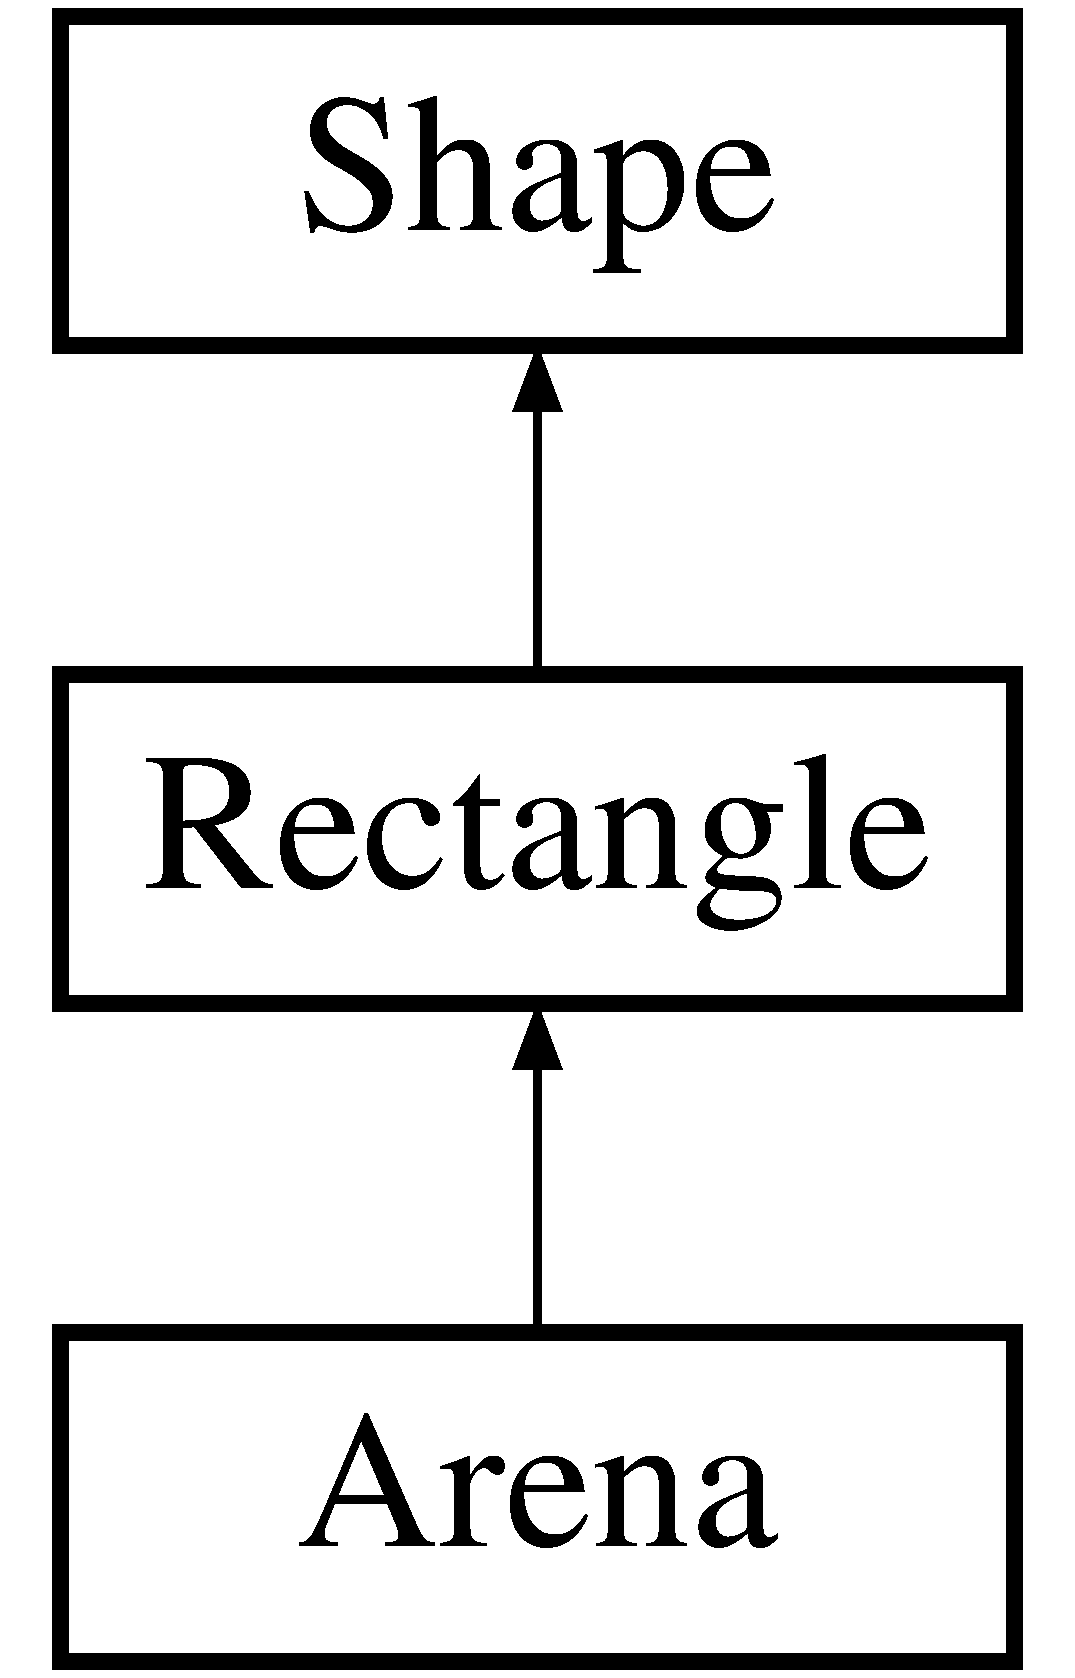
\includegraphics[height=2.000000cm]{class_arena}
\end{center}
\end{figure}
\subsection*{Public Member Functions}
\begin{DoxyCompactItemize}
\item 
\mbox{\Hypertarget{class_arena_aa37acdf43108ab0da04b77bbf79c2f7d}\label{class_arena_aa37acdf43108ab0da04b77bbf79c2f7d}} 
void {\bfseries find\+Arena} (const Mat \&img)
\item 
\mbox{\Hypertarget{class_arena_a67171d93c7aff0f9d8bd3ee0596e9033}\label{class_arena_a67171d93c7aff0f9d8bd3ee0596e9033}} 
std\+::vector$<$ cv\+::\+Point $>$ {\bfseries get\+Corners} ()
\item 
\mbox{\Hypertarget{class_arena_a7f822f33ff5810d4d266183e7606c0fe}\label{class_arena_a7f822f33ff5810d4d266183e7606c0fe}} 
void {\bfseries set\+Corners} (std\+::vector$<$ cv\+::\+Point $>$ corners)
\item 
\mbox{\Hypertarget{class_arena_ae7219e6d298213627a0c671e5c5f9536}\label{class_arena_ae7219e6d298213627a0c671e5c5f9536}} 
cv\+::\+Point {\bfseries get\+Top\+Left} ()
\item 
\mbox{\Hypertarget{class_arena_a7ab570cb7821df75c6da9af6491be034}\label{class_arena_a7ab570cb7821df75c6da9af6491be034}} 
void {\bfseries set\+Top\+Left} (cv\+::\+Point top\+Left)
\item 
\mbox{\Hypertarget{class_arena_aa417bc8757d66038038ac3f6a9d44860}\label{class_arena_aa417bc8757d66038038ac3f6a9d44860}} 
cv\+::\+Point {\bfseries get\+Top\+Right} ()
\item 
\mbox{\Hypertarget{class_arena_a82c7fa04e8acf52f6edecc1ee1c38001}\label{class_arena_a82c7fa04e8acf52f6edecc1ee1c38001}} 
void {\bfseries set\+Top\+Right} (cv\+::\+Point top\+Right)
\item 
\mbox{\Hypertarget{class_arena_afdd88e341c385561eafbc73e90e08404}\label{class_arena_afdd88e341c385561eafbc73e90e08404}} 
cv\+::\+Point {\bfseries get\+Bottom\+Left} ()
\item 
\mbox{\Hypertarget{class_arena_ac546db1983967fcc195369c8a0f1f9e5}\label{class_arena_ac546db1983967fcc195369c8a0f1f9e5}} 
void {\bfseries set\+Bottom\+Left} (cv\+::\+Point bottom\+Left)
\item 
\mbox{\Hypertarget{class_arena_ac62870a7bfa41baa7d38c4f7373cf3f5}\label{class_arena_ac62870a7bfa41baa7d38c4f7373cf3f5}} 
cv\+::\+Point {\bfseries get\+Bottom\+Right} ()
\item 
\mbox{\Hypertarget{class_arena_a2207ae5feab0d9ef8a19ab46fdd8685c}\label{class_arena_a2207ae5feab0d9ef8a19ab46fdd8685c}} 
void {\bfseries set\+Bottom\+Right} (cv\+::\+Point bottom\+Right)
\end{DoxyCompactItemize}


The documentation for this class was generated from the following file\+:\begin{DoxyCompactItemize}
\item 
Arena.\+hpp\end{DoxyCompactItemize}

\hypertarget{class_image_processing_1_1_calibration___instrinsic}{}\section{Image\+Processing\+:\+:Calibration\+\_\+\+Instrinsic Class Reference}
\label{class_image_processing_1_1_calibration___instrinsic}\index{Image\+Processing\+::\+Calibration\+\_\+\+Instrinsic@{Image\+Processing\+::\+Calibration\+\_\+\+Instrinsic}}


function that helps calibrating the camera resulting in an undistortion matrix  




{\ttfamily \#include $<$Calibration\+\_\+\+Intrinsic.\+hpp$>$}

\subsection*{Static Public Member Functions}
\begin{DoxyCompactItemize}
\item 
static void \mbox{\hyperlink{class_image_processing_1_1_calibration___instrinsic_acbaa653aac61aa9fc42696a51267b6b8}{perform\+Calibration}} (const std\+::string cali\+\_\+config)
\item 
static bool \mbox{\hyperlink{class_image_processing_1_1_calibration___instrinsic_a69ec772ab65d6fc5918a39b5e5839e2e}{run\+Calibration\+And\+Save}} (\mbox{\hyperlink{class_image_processing_1_1_settings}{Settings}} \&s, Size image\+Size, Mat \&camera\+Matrix, Mat \&dist\+Coeffs, std\+::vector$<$ std\+::vector$<$ Point2f $>$ $>$ image\+Points)
\item 
\mbox{\Hypertarget{class_image_processing_1_1_calibration___instrinsic_ad38f84410a98a93ed3c2078f06210880}\label{class_image_processing_1_1_calibration___instrinsic_ad38f84410a98a93ed3c2078f06210880}} 
static bool {\bfseries run\+Calibration} (\mbox{\hyperlink{class_image_processing_1_1_settings}{Settings}} \&s, Size \&image\+Size, Mat \&camera\+Matrix, Mat \&dist\+Coeffs, std\+::vector$<$ std\+::vector$<$ Point2f $>$ $>$ image\+Points, std\+::vector$<$ Mat $>$ \&rvecs, std\+::vector$<$ Mat $>$ \&tvecs, std\+::vector$<$ float $>$ \&reproj\+Errs, double \&total\+Avg\+Err)
\end{DoxyCompactItemize}


\subsection{Detailed Description}
function that helps calibrating the camera resulting in an undistortion matrix 

This class can be used to calibrate the distortion matrix. Given initial settings from a \mbox{\hyperlink{class_image_processing_1_1_settings}{Settings}} object and the opencv chessboard calibration tool it performs the calibration and saves the results in an external file.

\begin{DoxySeeAlso}{See also}
\mbox{\hyperlink{_settings_8hpp_source}{Settings.\+hpp}} 
\end{DoxySeeAlso}


\subsection{Member Function Documentation}
\mbox{\Hypertarget{class_image_processing_1_1_calibration___instrinsic_acbaa653aac61aa9fc42696a51267b6b8}\label{class_image_processing_1_1_calibration___instrinsic_acbaa653aac61aa9fc42696a51267b6b8}} 
\index{Image\+Processing\+::\+Calibration\+\_\+\+Instrinsic@{Image\+Processing\+::\+Calibration\+\_\+\+Instrinsic}!perform\+Calibration@{perform\+Calibration}}
\index{perform\+Calibration@{perform\+Calibration}!Image\+Processing\+::\+Calibration\+\_\+\+Instrinsic@{Image\+Processing\+::\+Calibration\+\_\+\+Instrinsic}}
\subsubsection{\texorpdfstring{perform\+Calibration()}{performCalibration()}}
{\footnotesize\ttfamily static void Image\+Processing\+::\+Calibration\+\_\+\+Instrinsic\+::perform\+Calibration (\begin{DoxyParamCaption}\item[{const std\+::string}]{cali\+\_\+config }\end{DoxyParamCaption})\hspace{0.3cm}{\ttfamily [static]}}

performs caliration and saves it to the filename indicated in the argument \begin{DoxyItemize}
\item cali\+\_\+config filename of finished calibration file \end{DoxyItemize}
\mbox{\Hypertarget{class_image_processing_1_1_calibration___instrinsic_a69ec772ab65d6fc5918a39b5e5839e2e}\label{class_image_processing_1_1_calibration___instrinsic_a69ec772ab65d6fc5918a39b5e5839e2e}} 
\index{Image\+Processing\+::\+Calibration\+\_\+\+Instrinsic@{Image\+Processing\+::\+Calibration\+\_\+\+Instrinsic}!run\+Calibration\+And\+Save@{run\+Calibration\+And\+Save}}
\index{run\+Calibration\+And\+Save@{run\+Calibration\+And\+Save}!Image\+Processing\+::\+Calibration\+\_\+\+Instrinsic@{Image\+Processing\+::\+Calibration\+\_\+\+Instrinsic}}
\subsubsection{\texorpdfstring{run\+Calibration\+And\+Save()}{runCalibrationAndSave()}}
{\footnotesize\ttfamily static bool Image\+Processing\+::\+Calibration\+\_\+\+Instrinsic\+::run\+Calibration\+And\+Save (\begin{DoxyParamCaption}\item[{\mbox{\hyperlink{class_image_processing_1_1_settings}{Settings}} \&}]{s,  }\item[{Size}]{image\+Size,  }\item[{Mat \&}]{camera\+Matrix,  }\item[{Mat \&}]{dist\+Coeffs,  }\item[{std\+::vector$<$ std\+::vector$<$ Point2f $>$ $>$}]{image\+Points }\end{DoxyParamCaption})\hspace{0.3cm}{\ttfamily [static]}}

Uses \mbox{\hyperlink{class_image_processing_1_1_settings}{Settings}} object to run and save the calibration \begin{DoxyItemize}
\item s \mbox{\hyperlink{class_image_processing_1_1_settings}{Settings}} object with information about chessboard and so on \item image\+Size \item camera\+Matrix \end{DoxyItemize}


The documentation for this class was generated from the following file\+:\begin{DoxyCompactItemize}
\item 
Calibration\+\_\+\+Intrinsic.\+hpp\end{DoxyCompactItemize}

\hypertarget{class_cell}{}\section{Cell Class Reference}
\label{class_cell}\index{Cell@{Cell}}
\subsection*{Public Member Functions}
\begin{DoxyCompactItemize}
\item 
\mbox{\Hypertarget{class_cell_a03becce6b307d86848e9563eb08ac2b3}\label{class_cell_a03becce6b307d86848e9563eb08ac2b3}} 
std\+::vector$<$ cv\+::\+Point $>$ {\bfseries get\+Corners} ()
\item 
\mbox{\Hypertarget{class_cell_a6d1ad0f2766cdd641ba0e65f8b3c9555}\label{class_cell_a6d1ad0f2766cdd641ba0e65f8b3c9555}} 
void {\bfseries set\+Corners} (std\+::vector$<$ cv\+::\+Point $>$ corners)
\item 
\mbox{\Hypertarget{class_cell_ac6e9338748b2098e034641c88a977b23}\label{class_cell_ac6e9338748b2098e034641c88a977b23}} 
cv\+::\+Point {\bfseries get\+Top\+Left} ()
\item 
\mbox{\Hypertarget{class_cell_a9e2d13652a170ef25265a41dfe39e93f}\label{class_cell_a9e2d13652a170ef25265a41dfe39e93f}} 
void {\bfseries set\+Top\+Left} (cv\+::\+Point top\+Left)
\item 
\mbox{\Hypertarget{class_cell_a4b08bffc22a4393fd86c9608d9723d7c}\label{class_cell_a4b08bffc22a4393fd86c9608d9723d7c}} 
cv\+::\+Point {\bfseries get\+Top\+Right} ()
\item 
\mbox{\Hypertarget{class_cell_a245afe36e263e2fbf66880e4ea628f40}\label{class_cell_a245afe36e263e2fbf66880e4ea628f40}} 
void {\bfseries set\+Top\+Right} (cv\+::\+Point top\+Right)
\item 
\mbox{\Hypertarget{class_cell_a1946142c5e112176e1cd20cc6d07f831}\label{class_cell_a1946142c5e112176e1cd20cc6d07f831}} 
cv\+::\+Point {\bfseries get\+Bottom\+Left} ()
\item 
\mbox{\Hypertarget{class_cell_a86387a50a4c3f641eede253ce6cfcddb}\label{class_cell_a86387a50a4c3f641eede253ce6cfcddb}} 
void {\bfseries set\+Bottom\+Left} (cv\+::\+Point bottom\+Left)
\item 
\mbox{\Hypertarget{class_cell_afa1704102095fd55ac036f7d290eed05}\label{class_cell_afa1704102095fd55ac036f7d290eed05}} 
cv\+::\+Point {\bfseries get\+Bottom\+Right} ()
\item 
\mbox{\Hypertarget{class_cell_ae68ff90cfde34cec208e8e74ce3f2745}\label{class_cell_ae68ff90cfde34cec208e8e74ce3f2745}} 
void {\bfseries set\+Bottom\+Right} (cv\+::\+Point bottom\+Right)
\item 
\mbox{\Hypertarget{class_cell_a6c7344ef2aa917e70364221bf86ff8bc}\label{class_cell_a6c7344ef2aa917e70364221bf86ff8bc}} 
bool {\bfseries is\+Empty} ()
\item 
\mbox{\Hypertarget{class_cell_aaf13f5d308c7f1eb670a050e4fc6dc28}\label{class_cell_aaf13f5d308c7f1eb670a050e4fc6dc28}} 
bool {\bfseries is\+Exit} ()
\item 
\mbox{\Hypertarget{class_cell_a34d62b7c65fd85f356bd9e2c3058edcb}\label{class_cell_a34d62b7c65fd85f356bd9e2c3058edcb}} 
bool {\bfseries is\+Border} ()
\item 
\mbox{\Hypertarget{class_cell_aee32093f779b1fa761b43a6b0a86ed6c}\label{class_cell_aee32093f779b1fa761b43a6b0a86ed6c}} 
bool {\bfseries is\+Obstacle} ()
\item 
\mbox{\Hypertarget{class_cell_ad86a719c04ff04bdf79c1c0b8e5a5942}\label{class_cell_ad86a719c04ff04bdf79c1c0b8e5a5942}} 
bool {\bfseries is\+Rescue} ()
\item 
\mbox{\Hypertarget{class_cell_a335c410074aaac9bb5594ea8adf648ff}\label{class_cell_a335c410074aaac9bb5594ea8adf648ff}} 
int {\bfseries get\+Digit} ()
\item 
\mbox{\Hypertarget{class_cell_a6047939b792e819bc2330151ff98864f}\label{class_cell_a6047939b792e819bc2330151ff98864f}} 
void {\bfseries set\+Empty} ()
\item 
\mbox{\Hypertarget{class_cell_a9fa0a3c17d798320c78bffe44411008e}\label{class_cell_a9fa0a3c17d798320c78bffe44411008e}} 
void {\bfseries set\+Exit} ()
\item 
\mbox{\Hypertarget{class_cell_aa690e62809d36d512cd39ccda9cea293}\label{class_cell_aa690e62809d36d512cd39ccda9cea293}} 
void {\bfseries set\+Border} ()
\item 
\mbox{\Hypertarget{class_cell_a34e953e7f720c3382f0b13c2480cafd0}\label{class_cell_a34e953e7f720c3382f0b13c2480cafd0}} 
void {\bfseries set\+Obstacle} ()
\item 
\mbox{\Hypertarget{class_cell_afa194cda3c1e8f9be100c9a14fda7f9d}\label{class_cell_afa194cda3c1e8f9be100c9a14fda7f9d}} 
void {\bfseries set\+Rescue} (int digit\+\_\+i)
\end{DoxyCompactItemize}


The documentation for this class was generated from the following file\+:\begin{DoxyCompactItemize}
\item 
Cell.\+hpp\end{DoxyCompactItemize}

\hypertarget{class_image_processing_1_1_character___recognition___algorithm}{}\section{Image\+Processing\+:\+:Character\+\_\+\+Recognition\+\_\+\+Algorithm Class Reference}
\label{class_image_processing_1_1_character___recognition___algorithm}\index{Image\+Processing\+::\+Character\+\_\+\+Recognition\+\_\+\+Algorithm@{Image\+Processing\+::\+Character\+\_\+\+Recognition\+\_\+\+Algorithm}}


abstract class for character recognition algorithms  




{\ttfamily \#include $<$Character\+\_\+\+Recognition\+\_\+\+Algorithm.\+hpp$>$}

Inheritance diagram for Image\+Processing\+:\+:Character\+\_\+\+Recognition\+\_\+\+Algorithm\+:\begin{figure}[H]
\begin{center}
\leavevmode
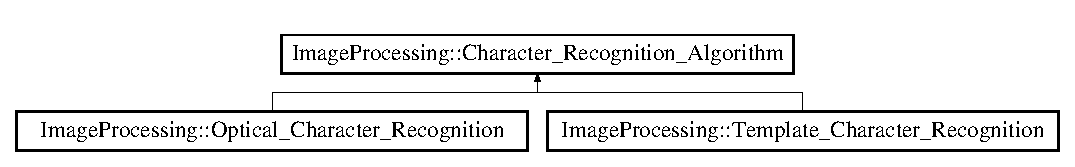
\includegraphics[height=1.794872cm]{class_image_processing_1_1_character___recognition___algorithm}
\end{center}
\end{figure}
\subsection*{Public Member Functions}
\begin{DoxyCompactItemize}
\item 
\mbox{\Hypertarget{class_image_processing_1_1_character___recognition___algorithm_aa90c50ea0e11c37d117ebbb69d859cf1}\label{class_image_processing_1_1_character___recognition___algorithm_aa90c50ea0e11c37d117ebbb69d859cf1}} 
void \mbox{\hyperlink{class_image_processing_1_1_character___recognition___algorithm_aa90c50ea0e11c37d117ebbb69d859cf1}{display\+Image}} (cv\+::\+Mat \&image, std\+::string window\+Title)
\begin{DoxyCompactList}\small\item\em calls cv\+::imshow \end{DoxyCompactList}\item 
\mbox{\Hypertarget{class_image_processing_1_1_character___recognition___algorithm_a7b42bfd91b6a9602106bc9445c880fda}\label{class_image_processing_1_1_character___recognition___algorithm_a7b42bfd91b6a9602106bc9445c880fda}} 
double \mbox{\hyperlink{class_image_processing_1_1_character___recognition___algorithm_a7b42bfd91b6a9602106bc9445c880fda}{determine\+\_\+orientation}} (cv\+::\+Mat image)
\begin{DoxyCompactList}\small\item\em computes an angle based on the fitline method \end{DoxyCompactList}\item 
\mbox{\Hypertarget{class_image_processing_1_1_character___recognition___algorithm_a2ece422da371975b49273b8b7ea2e285}\label{class_image_processing_1_1_character___recognition___algorithm_a2ece422da371975b49273b8b7ea2e285}} 
virtual std\+::pair$<$ int, int $>$ \mbox{\hyperlink{class_image_processing_1_1_character___recognition___algorithm_a2ece422da371975b49273b8b7ea2e285}{detect\+\_\+digit}} (cv\+::\+Mat \&image)=0
\begin{DoxyCompactList}\small\item\em the (virtual) function that runs the recognition engine \end{DoxyCompactList}\item 
\mbox{\Hypertarget{class_image_processing_1_1_character___recognition___algorithm_af251324381c75367abbc4a9d92eff4f9}\label{class_image_processing_1_1_character___recognition___algorithm_af251324381c75367abbc4a9d92eff4f9}} 
cv\+::\+Mat \mbox{\hyperlink{class_image_processing_1_1_character___recognition___algorithm_af251324381c75367abbc4a9d92eff4f9}{load\+Image}} (const std\+::string \&filename)
\begin{DoxyCompactList}\small\item\em calls cv\+::imread \end{DoxyCompactList}\item 
\mbox{\Hypertarget{class_image_processing_1_1_character___recognition___algorithm_a4b64167debaa2761914f08fceb6a3d7c}\label{class_image_processing_1_1_character___recognition___algorithm_a4b64167debaa2761914f08fceb6a3d7c}} 
void \mbox{\hyperlink{class_image_processing_1_1_character___recognition___algorithm_a4b64167debaa2761914f08fceb6a3d7c}{convert\+\_\+bgr\+\_\+to\+\_\+hsv}} (cv\+::\+Mat \&original, cv\+::\+Mat \&converted)
\begin{DoxyCompactList}\small\item\em convertion if color sheme \end{DoxyCompactList}\item 
\mbox{\Hypertarget{class_image_processing_1_1_character___recognition___algorithm_a3034cccb3aab0be8fe39c76faa3618be}\label{class_image_processing_1_1_character___recognition___algorithm_a3034cccb3aab0be8fe39c76faa3618be}} 
void \mbox{\hyperlink{class_image_processing_1_1_character___recognition___algorithm_a3034cccb3aab0be8fe39c76faa3618be}{apply\+\_\+mask}} (cv\+::\+Mat \&original, cv\+::\+Mat \&converted, cv\+::\+Scalar lowerbound, cv\+::\+Scalar upperbound)
\begin{DoxyCompactList}\small\item\em calls cv\+::inrange function \end{DoxyCompactList}\item 
\mbox{\Hypertarget{class_image_processing_1_1_character___recognition___algorithm_a71f57a3cccdc610b736f0a1144fa4a7f}\label{class_image_processing_1_1_character___recognition___algorithm_a71f57a3cccdc610b736f0a1144fa4a7f}} 
cv\+::\+Mat \mbox{\hyperlink{class_image_processing_1_1_character___recognition___algorithm_a71f57a3cccdc610b736f0a1144fa4a7f}{apply\+\_\+some\+\_\+filtering}} (cv\+::\+Mat \&img)
\begin{DoxyCompactList}\small\item\em dilate and erode image \end{DoxyCompactList}\item 
\mbox{\Hypertarget{class_image_processing_1_1_character___recognition___algorithm_a9f546a88cdebb36ef0128537e02f5a80}\label{class_image_processing_1_1_character___recognition___algorithm_a9f546a88cdebb36ef0128537e02f5a80}} 
void \mbox{\hyperlink{class_image_processing_1_1_character___recognition___algorithm_a9f546a88cdebb36ef0128537e02f5a80}{prepare\+\_\+uniform\+\_\+window}} (cv\+::\+Mat \&img)
\begin{DoxyCompactList}\small\item\em resizing to 200x200px, threshold, erode and blur \end{DoxyCompactList}\item 
\mbox{\Hypertarget{class_image_processing_1_1_character___recognition___algorithm_a7552eb21dca6acfa702518ae36e3de8b}\label{class_image_processing_1_1_character___recognition___algorithm_a7552eb21dca6acfa702518ae36e3de8b}} 
std\+::vector$<$ cv\+::\+Rect $>$ \mbox{\hyperlink{class_image_processing_1_1_character___recognition___algorithm_a7552eb21dca6acfa702518ae36e3de8b}{extract\+\_\+regions\+\_\+of\+\_\+interest}} (cv\+::\+Mat \&original\+\_\+img, cv\+::\+Mat \&filtered\+\_\+img, cv\+::\+Mat \&returned\+Img)
\begin{DoxyCompactList}\small\item\em extract regions that circular \end{DoxyCompactList}\item 
\mbox{\Hypertarget{class_image_processing_1_1_character___recognition___algorithm_af4e813e7e622253bd1fa1f3253f80816}\label{class_image_processing_1_1_character___recognition___algorithm_af4e813e7e622253bd1fa1f3253f80816}} 
std\+::tuple$<$ cv\+::\+Mat, cv\+::\+Mat $>$ \mbox{\hyperlink{class_image_processing_1_1_character___recognition___algorithm_af4e813e7e622253bd1fa1f3253f80816}{invert\+\_\+masked\+\_\+image}} (cv\+::\+Mat \&original, cv\+::\+Mat \&masked\+\_\+image)
\begin{DoxyCompactList}\small\item\em inverts the image colors black white -\/ white black \end{DoxyCompactList}\item 
\mbox{\Hypertarget{class_image_processing_1_1_character___recognition___algorithm_a08d3f01496729b439e68819e61a564e5}\label{class_image_processing_1_1_character___recognition___algorithm_a08d3f01496729b439e68819e61a564e5}} 
void \mbox{\hyperlink{class_image_processing_1_1_character___recognition___algorithm_a08d3f01496729b439e68819e61a564e5}{rotate\+\_\+image}} (cv\+::\+Mat \&src, double angle, cv\+::\+Mat \&result)
\begin{DoxyCompactList}\small\item\em rotates the image and produces a new image with black background \end{DoxyCompactList}\item 
\mbox{\Hypertarget{class_image_processing_1_1_character___recognition___algorithm_a649e7aeabaa4bc0350ad13a053e4e720}\label{class_image_processing_1_1_character___recognition___algorithm_a649e7aeabaa4bc0350ad13a053e4e720}} 
std\+::vector$<$ cv\+::\+Mat $>$ \mbox{\hyperlink{class_image_processing_1_1_character___recognition___algorithm_a649e7aeabaa4bc0350ad13a053e4e720}{preprocessing}} (cv\+::\+Mat \&img, cv\+::\+Mat \&filtered, std\+::vector$<$ cv\+::\+Rect $>$ \&bound\+Rect)
\begin{DoxyCompactList}\small\item\em applies the color filter and detects circular objects and returns images of found regions \end{DoxyCompactList}\item 
\mbox{\Hypertarget{class_image_processing_1_1_character___recognition___algorithm_abf787b74e22f19882892b0542ed8451f}\label{class_image_processing_1_1_character___recognition___algorithm_abf787b74e22f19882892b0542ed8451f}} 
void \mbox{\hyperlink{class_image_processing_1_1_character___recognition___algorithm_abf787b74e22f19882892b0542ed8451f}{set\+\_\+lower\+\_\+bound\+\_\+filter}} (double hue, double saturation, double value)
\begin{DoxyCompactList}\small\item\em set the lower value for filter \end{DoxyCompactList}\item 
\mbox{\Hypertarget{class_image_processing_1_1_character___recognition___algorithm_ae46d414c856535dd69b51b2cd80ec486}\label{class_image_processing_1_1_character___recognition___algorithm_ae46d414c856535dd69b51b2cd80ec486}} 
void \mbox{\hyperlink{class_image_processing_1_1_character___recognition___algorithm_ae46d414c856535dd69b51b2cd80ec486}{set\+\_\+upper\+\_\+bound\+\_\+filter}} (double hue, double saturation, double value)
\begin{DoxyCompactList}\small\item\em set the upper value for filter \end{DoxyCompactList}\item 
\mbox{\Hypertarget{class_image_processing_1_1_character___recognition___algorithm_a66568e425dfb386f8a78326867b628fd}\label{class_image_processing_1_1_character___recognition___algorithm_a66568e425dfb386f8a78326867b628fd}} 
void \mbox{\hyperlink{class_image_processing_1_1_character___recognition___algorithm_a66568e425dfb386f8a78326867b628fd}{turn\+\_\+image}} (cv\+::\+Mat input, cv\+::\+Mat \&output, double angle)
\begin{DoxyCompactList}\small\item\em calls rotate image \end{DoxyCompactList}\end{DoxyCompactItemize}
\subsection*{Public Attributes}
\begin{DoxyCompactItemize}
\item 
\mbox{\Hypertarget{class_image_processing_1_1_character___recognition___algorithm_aa3104edea691e7202e2abe0c044dabbe}\label{class_image_processing_1_1_character___recognition___algorithm_aa3104edea691e7202e2abe0c044dabbe}} 
const double {\bfseries M\+I\+N\+\_\+\+A\+R\+E\+A\+\_\+\+S\+I\+ZE} = 200
\item 
\mbox{\Hypertarget{class_image_processing_1_1_character___recognition___algorithm_adc5636619442cbfa3e276210a914b3f6}\label{class_image_processing_1_1_character___recognition___algorithm_adc5636619442cbfa3e276210a914b3f6}} 
\mbox{\hyperlink{struct_image_processing_1_1_h_s_v_filter_range}{H\+S\+V\+Filter\+Range}} {\bfseries filter} = \mbox{\hyperlink{struct_image_processing_1_1_h_s_v_filter_range}{H\+S\+V\+Filter\+Range}}()
\item 
\mbox{\Hypertarget{class_image_processing_1_1_character___recognition___algorithm_afbab64ce9fff483a75b4533db4392f81}\label{class_image_processing_1_1_character___recognition___algorithm_afbab64ce9fff483a75b4533db4392f81}} 
double \mbox{\hyperlink{class_image_processing_1_1_character___recognition___algorithm_afbab64ce9fff483a75b4533db4392f81}{delta\+\_\+angle}} = 30
\begin{DoxyCompactList}\small\item\em angle by which the image is turned each step from 0 to 360 degrees to find the right orientation \end{DoxyCompactList}\item 
\mbox{\Hypertarget{class_image_processing_1_1_character___recognition___algorithm_ac166463ea5fc4bf892dc2035467351ea}\label{class_image_processing_1_1_character___recognition___algorithm_ac166463ea5fc4bf892dc2035467351ea}} 
unsigned int \mbox{\hyperlink{class_image_processing_1_1_character___recognition___algorithm_ac166463ea5fc4bf892dc2035467351ea}{suf\+\_\+conf}} = 80
\begin{DoxyCompactList}\small\item\em sufficient confidence value to stop the rotating wheel of the digit recognition \end{DoxyCompactList}\end{DoxyCompactItemize}


\subsection{Detailed Description}
abstract class for character recognition algorithms 

The documentation for this class was generated from the following file\+:\begin{DoxyCompactItemize}
\item 
Character\+\_\+\+Recognition\+\_\+\+Algorithm.\+hpp\end{DoxyCompactItemize}

\hypertarget{class_geometry2_d_1_1_circle}{}\section{Geometry2D\+:\+:Circle Class Reference}
\label{class_geometry2_d_1_1_circle}\index{Geometry2\+D\+::\+Circle@{Geometry2\+D\+::\+Circle}}


\mbox{\hyperlink{class_geometry2_d_1_1_circle}{Circle}} class is able to detect and save the arena given a photo.  




{\ttfamily \#include $<$Circle.\+hpp$>$}

Inheritance diagram for Geometry2D\+:\+:Circle\+:\begin{figure}[H]
\begin{center}
\leavevmode
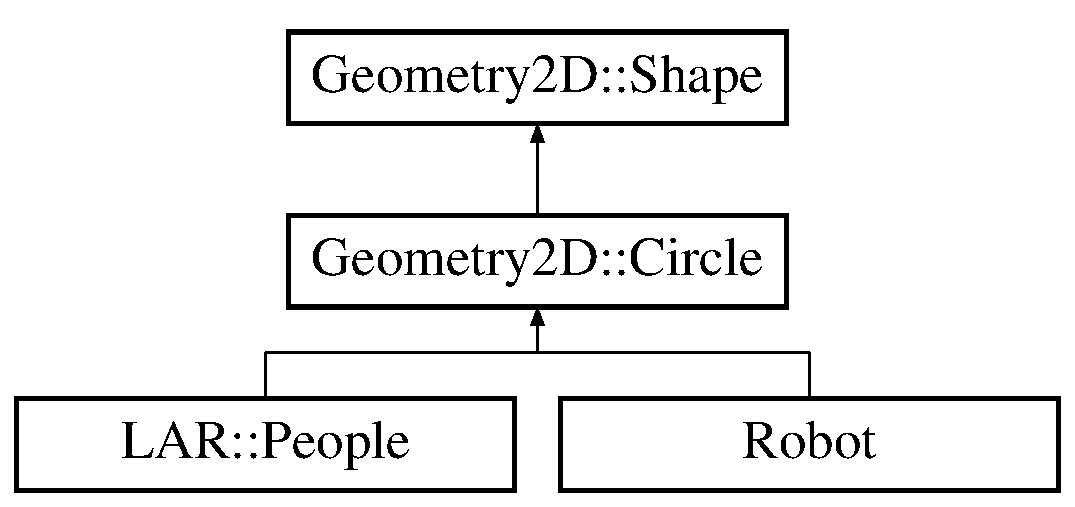
\includegraphics[height=3.000000cm]{class_geometry2_d_1_1_circle}
\end{center}
\end{figure}
\subsection*{Public Member Functions}
\begin{DoxyCompactItemize}
\item 
\mbox{\hyperlink{class_geometry2_d_1_1_circle_a8e740ff9413a9abac8f7c666b89c4366}{Circle}} ()
\item 
\mbox{\hyperlink{class_geometry2_d_1_1_circle_ae5bfc08e732dd97fc3cc4c485787be44}{$\sim$\+Circle}} ()
\item 
int \mbox{\hyperlink{class_geometry2_d_1_1_circle_a93adf6a4690d211a16800d0ddbeb9949}{get\+Radius}} ()
\item 
void \mbox{\hyperlink{class_geometry2_d_1_1_circle_acdeabe8582b65611dbc117cdc7604f18}{set\+Radius}} (int radius\+\_\+c)
\item 
cv\+::\+Point \mbox{\hyperlink{class_geometry2_d_1_1_circle_ad6605cfef3530b9185213f694c9fca6a}{get\+Center}} ()
\item 
void \mbox{\hyperlink{class_geometry2_d_1_1_circle_a1d73cfc9f0e4fe3eb8a93e2a5a4f0ffd}{set\+Center}} (cv\+::\+Point center\+\_\+c)
\end{DoxyCompactItemize}
\subsection*{Public Attributes}
\begin{DoxyCompactItemize}
\item 
\mbox{\Hypertarget{class_geometry2_d_1_1_circle_abdc47cda7bbabe42e10536a29952c2fa}\label{class_geometry2_d_1_1_circle_abdc47cda7bbabe42e10536a29952c2fa}} 
cv\+::\+Point {\bfseries center}
\item 
\mbox{\Hypertarget{class_geometry2_d_1_1_circle_a9f62fa67d77dac2856f0b8971f13b7e6}\label{class_geometry2_d_1_1_circle_a9f62fa67d77dac2856f0b8971f13b7e6}} 
double {\bfseries radius}
\end{DoxyCompactItemize}


\subsection{Detailed Description}
\mbox{\hyperlink{class_geometry2_d_1_1_circle}{Circle}} class is able to detect and save the arena given a photo. 

\subsection{Constructor \& Destructor Documentation}
\mbox{\Hypertarget{class_geometry2_d_1_1_circle_a8e740ff9413a9abac8f7c666b89c4366}\label{class_geometry2_d_1_1_circle_a8e740ff9413a9abac8f7c666b89c4366}} 
\index{Geometry2\+D\+::\+Circle@{Geometry2\+D\+::\+Circle}!Circle@{Circle}}
\index{Circle@{Circle}!Geometry2\+D\+::\+Circle@{Geometry2\+D\+::\+Circle}}
\subsubsection{\texorpdfstring{Circle()}{Circle()}}
{\footnotesize\ttfamily Geometry2\+D\+::\+Circle\+::\+Circle (\begin{DoxyParamCaption}{ }\end{DoxyParamCaption})}

constructor of \mbox{\hyperlink{class_geometry2_d_1_1_circle}{Circle}} class \mbox{\Hypertarget{class_geometry2_d_1_1_circle_ae5bfc08e732dd97fc3cc4c485787be44}\label{class_geometry2_d_1_1_circle_ae5bfc08e732dd97fc3cc4c485787be44}} 
\index{Geometry2\+D\+::\+Circle@{Geometry2\+D\+::\+Circle}!````~Circle@{$\sim$\+Circle}}
\index{````~Circle@{$\sim$\+Circle}!Geometry2\+D\+::\+Circle@{Geometry2\+D\+::\+Circle}}
\subsubsection{\texorpdfstring{$\sim$\+Circle()}{~Circle()}}
{\footnotesize\ttfamily Geometry2\+D\+::\+Circle\+::$\sim$\+Circle (\begin{DoxyParamCaption}{ }\end{DoxyParamCaption})}

destructor of \mbox{\hyperlink{class_geometry2_d_1_1_circle}{Circle}} class 

\subsection{Member Function Documentation}
\mbox{\Hypertarget{class_geometry2_d_1_1_circle_ad6605cfef3530b9185213f694c9fca6a}\label{class_geometry2_d_1_1_circle_ad6605cfef3530b9185213f694c9fca6a}} 
\index{Geometry2\+D\+::\+Circle@{Geometry2\+D\+::\+Circle}!get\+Center@{get\+Center}}
\index{get\+Center@{get\+Center}!Geometry2\+D\+::\+Circle@{Geometry2\+D\+::\+Circle}}
\subsubsection{\texorpdfstring{get\+Center()}{getCenter()}}
{\footnotesize\ttfamily cv\+::\+Point Geometry2\+D\+::\+Circle\+::get\+Center (\begin{DoxyParamCaption}{ }\end{DoxyParamCaption})}

return the center of the circle \begin{DoxyReturn}{Returns}
the center of the circle 
\end{DoxyReturn}
\mbox{\Hypertarget{class_geometry2_d_1_1_circle_a93adf6a4690d211a16800d0ddbeb9949}\label{class_geometry2_d_1_1_circle_a93adf6a4690d211a16800d0ddbeb9949}} 
\index{Geometry2\+D\+::\+Circle@{Geometry2\+D\+::\+Circle}!get\+Radius@{get\+Radius}}
\index{get\+Radius@{get\+Radius}!Geometry2\+D\+::\+Circle@{Geometry2\+D\+::\+Circle}}
\subsubsection{\texorpdfstring{get\+Radius()}{getRadius()}}
{\footnotesize\ttfamily int Geometry2\+D\+::\+Circle\+::get\+Radius (\begin{DoxyParamCaption}{ }\end{DoxyParamCaption})}

return the radius of the circle \begin{DoxyReturn}{Returns}
the radius of the circle 
\end{DoxyReturn}
\mbox{\Hypertarget{class_geometry2_d_1_1_circle_a1d73cfc9f0e4fe3eb8a93e2a5a4f0ffd}\label{class_geometry2_d_1_1_circle_a1d73cfc9f0e4fe3eb8a93e2a5a4f0ffd}} 
\index{Geometry2\+D\+::\+Circle@{Geometry2\+D\+::\+Circle}!set\+Center@{set\+Center}}
\index{set\+Center@{set\+Center}!Geometry2\+D\+::\+Circle@{Geometry2\+D\+::\+Circle}}
\subsubsection{\texorpdfstring{set\+Center()}{setCenter()}}
{\footnotesize\ttfamily void Geometry2\+D\+::\+Circle\+::set\+Center (\begin{DoxyParamCaption}\item[{cv\+::\+Point}]{center\+\_\+c }\end{DoxyParamCaption})}

set the center of the circle 
\begin{DoxyParams}{Parameters}
{\em center\+\_\+c} & center of the circle \\
\hline
\end{DoxyParams}
\mbox{\Hypertarget{class_geometry2_d_1_1_circle_acdeabe8582b65611dbc117cdc7604f18}\label{class_geometry2_d_1_1_circle_acdeabe8582b65611dbc117cdc7604f18}} 
\index{Geometry2\+D\+::\+Circle@{Geometry2\+D\+::\+Circle}!set\+Radius@{set\+Radius}}
\index{set\+Radius@{set\+Radius}!Geometry2\+D\+::\+Circle@{Geometry2\+D\+::\+Circle}}
\subsubsection{\texorpdfstring{set\+Radius()}{setRadius()}}
{\footnotesize\ttfamily void Geometry2\+D\+::\+Circle\+::set\+Radius (\begin{DoxyParamCaption}\item[{int}]{radius\+\_\+c }\end{DoxyParamCaption})}

set the radius of the circle 
\begin{DoxyParams}{Parameters}
{\em radius\+\_\+c} & the radius of the circle \\
\hline
\end{DoxyParams}


The documentation for this class was generated from the following file\+:\begin{DoxyCompactItemize}
\item 
Circle.\+hpp\end{DoxyCompactItemize}

\hypertarget{class_path2_d_1_1_element_1_1_circular_line}{}\section{Path2D\+:\+:Element\+:\+:Circular\+Line Class Reference}
\label{class_path2_d_1_1_element_1_1_circular_line}\index{Path2\+D\+::\+Element\+::\+Circular\+Line@{Path2\+D\+::\+Element\+::\+Circular\+Line}}


Class for managing circle in the pat.  




{\ttfamily \#include $<$Circular\+Line.\+hpp$>$}

Inheritance diagram for Path2D\+:\+:Element\+:\+:Circular\+Line\+:\begin{figure}[H]
\begin{center}
\leavevmode
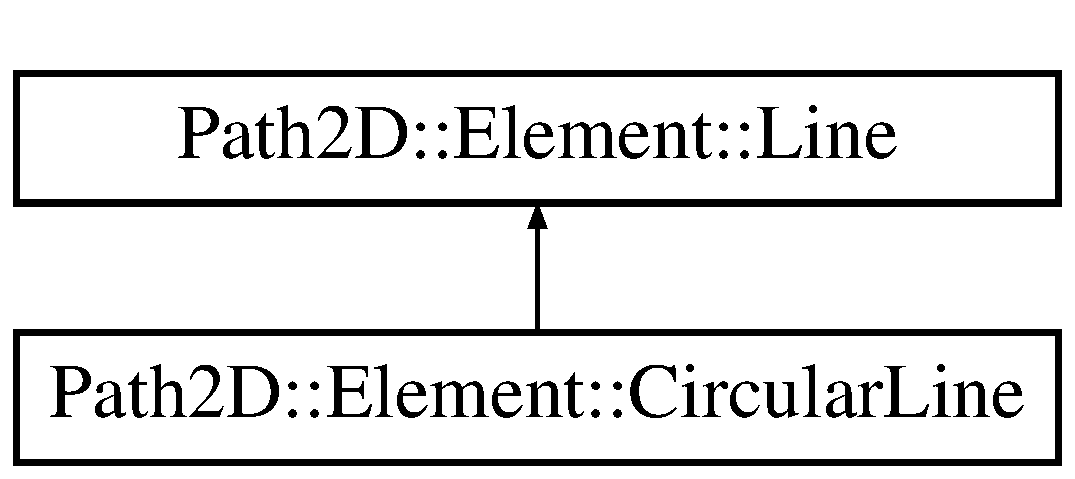
\includegraphics[height=2.000000cm]{class_path2_d_1_1_element_1_1_circular_line}
\end{center}
\end{figure}
\subsection*{Public Member Functions}
\begin{DoxyCompactItemize}
\item 
\mbox{\hyperlink{class_path2_d_1_1_element_1_1_circular_line_acb8d63253b111784eb95dd1ae77ba083}{Circular\+Line}} (\mbox{\hyperlink{class_path2_d_1_1_element_1_1_position}{Position}} start\+\_\+point, double curvature, double length)
\begin{DoxyCompactList}\small\item\em constructor of the class \end{DoxyCompactList}\item 
\mbox{\Hypertarget{class_path2_d_1_1_element_1_1_circular_line_a63a787df3c97311f78dd6ad8cfbb3a3b}\label{class_path2_d_1_1_element_1_1_circular_line_a63a787df3c97311f78dd6ad8cfbb3a3b}} 
\mbox{\hyperlink{class_path2_d_1_1_element_1_1_circular_line_a63a787df3c97311f78dd6ad8cfbb3a3b}{$\sim$\+Circular\+Line}} ()
\begin{DoxyCompactList}\small\item\em destructor of the class \end{DoxyCompactList}\end{DoxyCompactItemize}


\subsection{Detailed Description}
Class for managing circle in the pat. 

\subsection{Constructor \& Destructor Documentation}
\mbox{\Hypertarget{class_path2_d_1_1_element_1_1_circular_line_acb8d63253b111784eb95dd1ae77ba083}\label{class_path2_d_1_1_element_1_1_circular_line_acb8d63253b111784eb95dd1ae77ba083}} 
\index{Path2\+D\+::\+Element\+::\+Circular\+Line@{Path2\+D\+::\+Element\+::\+Circular\+Line}!Circular\+Line@{Circular\+Line}}
\index{Circular\+Line@{Circular\+Line}!Path2\+D\+::\+Element\+::\+Circular\+Line@{Path2\+D\+::\+Element\+::\+Circular\+Line}}
\subsubsection{\texorpdfstring{Circular\+Line()}{CircularLine()}}
{\footnotesize\ttfamily Path2\+D\+::\+Element\+::\+Circular\+Line\+::\+Circular\+Line (\begin{DoxyParamCaption}\item[{\mbox{\hyperlink{class_path2_d_1_1_element_1_1_position}{Position}}}]{start\+\_\+point,  }\item[{double}]{curvature,  }\item[{double}]{length }\end{DoxyParamCaption})}



constructor of the class 


\begin{DoxyParams}{Parameters}
{\em start\+\_\+point} & start position of the line \\
\hline
{\em curvature} & curvature of the path \\
\hline
{\em length} & length of the path \\
\hline
\end{DoxyParams}


The documentation for this class was generated from the following file\+:\begin{DoxyCompactItemize}
\item 
Circular\+Line.\+hpp\end{DoxyCompactItemize}

\hypertarget{class_image_processing_1_1_clipper}{}\section{Image\+Processing\+:\+:Clipper Class Reference}
\label{class_image_processing_1_1_clipper}\index{Image\+Processing\+::\+Clipper@{Image\+Processing\+::\+Clipper}}
\subsection*{Public Member Functions}
\begin{DoxyCompactItemize}
\item 
std\+::vector$<$ cv\+::\+Point $>$ \mbox{\hyperlink{class_image_processing_1_1_clipper_a936e548aa6e5f9be99617c4d3df3e322}{clip}} (std\+::vector$<$ cv\+::\+Point $>$ \&points, int offset)
\item 
\mbox{\Hypertarget{class_image_processing_1_1_clipper_a8d9c87e875b84b07677f515e11c29fab}\label{class_image_processing_1_1_clipper_a8d9c87e875b84b07677f515e11c29fab}} 
std\+::vector$<$ cv\+::\+Point $>$ {\bfseries clip\+Arena} (std\+::vector$<$ cv\+::\+Point $>$ \&points, int offset)
\end{DoxyCompactItemize}


\subsection{Member Function Documentation}
\mbox{\Hypertarget{class_image_processing_1_1_clipper_a936e548aa6e5f9be99617c4d3df3e322}\label{class_image_processing_1_1_clipper_a936e548aa6e5f9be99617c4d3df3e322}} 
\index{Image\+Processing\+::\+Clipper@{Image\+Processing\+::\+Clipper}!clip@{clip}}
\index{clip@{clip}!Image\+Processing\+::\+Clipper@{Image\+Processing\+::\+Clipper}}
\subsubsection{\texorpdfstring{clip()}{clip()}}
{\footnotesize\ttfamily std\+::vector$<$cv\+::\+Point$>$ Image\+Processing\+::\+Clipper\+::clip (\begin{DoxyParamCaption}\item[{std\+::vector$<$ cv\+::\+Point $>$ \&}]{points,  }\item[{int}]{offset }\end{DoxyParamCaption})}

given a list of point and an offster perform clipping and return a vector of points 
\begin{DoxyParams}{Parameters}
{\em points} & list of input points \\
\hline
{\em offset} & offset values \\
\hline
\end{DoxyParams}
\begin{DoxyReturn}{Returns}
vector of points after clipping 
\end{DoxyReturn}


The documentation for this class was generated from the following file\+:\begin{DoxyCompactItemize}
\item 
Clipper.\+hpp\end{DoxyCompactItemize}

\hypertarget{class_path2_d_1_1_path_finder_1_1_collision_detector}{}\section{Path2D\+:\+:Path\+Finder\+:\+:Collision\+Detector Class Reference}
\label{class_path2_d_1_1_path_finder_1_1_collision_detector}\index{Path2\+D\+::\+Path\+Finder\+::\+Collision\+Detector@{Path2\+D\+::\+Path\+Finder\+::\+Collision\+Detector}}


detector of collision between obstacles and path  




{\ttfamily \#include $<$Path\+Finder.\+hpp$>$}

\subsection*{Public Member Functions}
\begin{DoxyCompactItemize}
\item 
\mbox{\Hypertarget{class_path2_d_1_1_path_finder_1_1_collision_detector_ab0dd27f4e4b0e901be9ad1ef7c938949}\label{class_path2_d_1_1_path_finder_1_1_collision_detector_ab0dd27f4e4b0e901be9ad1ef7c938949}} 
\mbox{\hyperlink{class_path2_d_1_1_path_finder_1_1_collision_detector_ab0dd27f4e4b0e901be9ad1ef7c938949}{Collision\+Detector}} ()
\begin{DoxyCompactList}\small\item\em constructor of Collision\+Detector\+\_\+hpp class \end{DoxyCompactList}\item 
\mbox{\Hypertarget{class_path2_d_1_1_path_finder_1_1_collision_detector_a978b6fc7e1d64833e0feb22c41db1383}\label{class_path2_d_1_1_path_finder_1_1_collision_detector_a978b6fc7e1d64833e0feb22c41db1383}} 
\mbox{\hyperlink{class_path2_d_1_1_path_finder_1_1_collision_detector_a978b6fc7e1d64833e0feb22c41db1383}{$\sim$\+Collision\+Detector}} ()
\begin{DoxyCompactList}\small\item\em destructor of Collision\+Detector\+\_\+hpp class \end{DoxyCompactList}\item 
std\+::pair$<$ bool, \mbox{\hyperlink{class_cell}{Cell}} $\ast$ $>$ \mbox{\hyperlink{class_path2_d_1_1_path_finder_1_1_collision_detector_a3ff8fb92d990f44157c0b2469b1c9a24}{detect\+Collision}} (std\+::vector$<$ \mbox{\hyperlink{class_path2_d_1_1_element_1_1_line}{Line}} $>$ \&lines\+\_\+i, \mbox{\hyperlink{class_map}{Map}} $\ast$map, double max\+\_\+curvature)
\begin{DoxyCompactList}\small\item\em given a vector of lines detect if the path is feasible \end{DoxyCompactList}\end{DoxyCompactItemize}


\subsection{Detailed Description}
detector of collision between obstacles and path 

\subsection{Member Function Documentation}
\mbox{\Hypertarget{class_path2_d_1_1_path_finder_1_1_collision_detector_a3ff8fb92d990f44157c0b2469b1c9a24}\label{class_path2_d_1_1_path_finder_1_1_collision_detector_a3ff8fb92d990f44157c0b2469b1c9a24}} 
\index{Path2\+D\+::\+Path\+Finder\+::\+Collision\+Detector@{Path2\+D\+::\+Path\+Finder\+::\+Collision\+Detector}!detect\+Collision@{detect\+Collision}}
\index{detect\+Collision@{detect\+Collision}!Path2\+D\+::\+Path\+Finder\+::\+Collision\+Detector@{Path2\+D\+::\+Path\+Finder\+::\+Collision\+Detector}}
\subsubsection{\texorpdfstring{detect\+Collision()}{detectCollision()}}
{\footnotesize\ttfamily std\+::pair$<$bool,\mbox{\hyperlink{class_cell}{Cell}}$\ast$$>$ Path2\+D\+::\+Path\+Finder\+::\+Collision\+Detector\+::detect\+Collision (\begin{DoxyParamCaption}\item[{std\+::vector$<$ \mbox{\hyperlink{class_path2_d_1_1_element_1_1_line}{Line}} $>$ \&}]{lines\+\_\+i,  }\item[{\mbox{\hyperlink{class_map}{Map}} $\ast$}]{map,  }\item[{double}]{max\+\_\+curvature }\end{DoxyParamCaption})}



given a vector of lines detect if the path is feasible 


\begin{DoxyParams}{Parameters}
{\em lines\+\_\+i} & vector of line that we want to check \\
\hline
{\em map} & map of the arena \\
\hline
{\em max\+\_\+curvature} & curvature of the path \\
\hline
\end{DoxyParams}
\begin{DoxyReturn}{Returns}
true if there is a collision false otherwise 
\end{DoxyReturn}


The documentation for this class was generated from the following file\+:\begin{DoxyCompactItemize}
\item 
Path\+Finder.\+hpp\end{DoxyCompactItemize}

\hypertarget{class_image_processing_1_1_color___processing}{}\section{Image\+Processing\+:\+:Color\+\_\+\+Processing Class Reference}
\label{class_image_processing_1_1_color___processing}\index{Image\+Processing\+::\+Color\+\_\+\+Processing@{Image\+Processing\+::\+Color\+\_\+\+Processing}}


A class that helps to extract information about the color values of pixels in an image.  




{\ttfamily \#include $<$Color\+\_\+\+Processing.\+hpp$>$}

\subsection*{Public Member Functions}
\begin{DoxyCompactItemize}
\item 
\mbox{\Hypertarget{class_image_processing_1_1_color___processing_ae6357f66cadc70bb8f087cf9b0222cd2}\label{class_image_processing_1_1_color___processing_ae6357f66cadc70bb8f087cf9b0222cd2}} 
void \mbox{\hyperlink{class_image_processing_1_1_color___processing_ae6357f66cadc70bb8f087cf9b0222cd2}{load\+\_\+pixels}} (cv\+::\+Mat \&img)
\begin{DoxyCompactList}\small\item\em load all relevant pixels for evaluation \end{DoxyCompactList}\item 
\mbox{\Hypertarget{class_image_processing_1_1_color___processing_a34be73aacbf881359947e4e323779bc7}\label{class_image_processing_1_1_color___processing_a34be73aacbf881359947e4e323779bc7}} 
\mbox{\hyperlink{struct_image_processing_1_1_h_s_v_filter_range}{H\+S\+V\+Filter\+Range}} \mbox{\hyperlink{class_image_processing_1_1_color___processing_a34be73aacbf881359947e4e323779bc7}{get\+Filter}} ()
\begin{DoxyCompactList}\small\item\em creating and return an \mbox{\hyperlink{struct_image_processing_1_1_h_s_v_filter_range}{H\+S\+V\+Filter\+Range}} filter object \end{DoxyCompactList}\item 
\mbox{\Hypertarget{class_image_processing_1_1_color___processing_a9ee0aca190f2e0bcbacadfdcb5d3f98f}\label{class_image_processing_1_1_color___processing_a9ee0aca190f2e0bcbacadfdcb5d3f98f}} 
void \mbox{\hyperlink{class_image_processing_1_1_color___processing_a9ee0aca190f2e0bcbacadfdcb5d3f98f}{find\+\_\+black\+\_\+threshold}} (cv\+::\+Mat \&img)
\begin{DoxyCompactList}\small\item\em find the lower values of s and v \end{DoxyCompactList}\item 
\mbox{\Hypertarget{class_image_processing_1_1_color___processing_a3e1aee532a7df264fde28dfdbafba4d5}\label{class_image_processing_1_1_color___processing_a3e1aee532a7df264fde28dfdbafba4d5}} 
void \mbox{\hyperlink{class_image_processing_1_1_color___processing_a3e1aee532a7df264fde28dfdbafba4d5}{calibrate\+\_\+color}} (const std\+::string filename)
\begin{DoxyCompactList}\small\item\em use an image to create a color filter \end{DoxyCompactList}\item 
\mbox{\Hypertarget{class_image_processing_1_1_color___processing_ab0075249337c1147d6425a1899a16464}\label{class_image_processing_1_1_color___processing_ab0075249337c1147d6425a1899a16464}} 
void \mbox{\hyperlink{class_image_processing_1_1_color___processing_ab0075249337c1147d6425a1899a16464}{demo}} (cv\+::\+Mat \&img)
\begin{DoxyCompactList}\small\item\em a demo function \end{DoxyCompactList}\end{DoxyCompactItemize}
\subsection*{Public Attributes}
\begin{DoxyCompactItemize}
\item 
\mbox{\Hypertarget{class_image_processing_1_1_color___processing_a8a027ab4f4c0a4736ff78785c172affd}\label{class_image_processing_1_1_color___processing_a8a027ab4f4c0a4736ff78785c172affd}} 
std\+::pair$<$ double, double $>$ \mbox{\hyperlink{class_image_processing_1_1_color___processing_a8a027ab4f4c0a4736ff78785c172affd}{range}} = std\+::pair$<$double,double$>$ (0,0)
\begin{DoxyCompactList}\small\item\em when implemeting a black filter the lowest SV values are stored in the range \end{DoxyCompactList}\item 
\mbox{\Hypertarget{class_image_processing_1_1_color___processing_a42ac41f06222b9175e029516e39d24d9}\label{class_image_processing_1_1_color___processing_a42ac41f06222b9175e029516e39d24d9}} 
std\+::pair$<$ double, double $>$ \mbox{\hyperlink{class_image_processing_1_1_color___processing_a42ac41f06222b9175e029516e39d24d9}{black\+\_\+threshold}} = std\+::pair$<$double,double$>$ (0,0)
\begin{DoxyCompactList}\small\item\em the givent threshold -\/ acts like an additional black filter \end{DoxyCompactList}\item 
\mbox{\Hypertarget{class_image_processing_1_1_color___processing_a0f409e933954d9a45d82886264842529}\label{class_image_processing_1_1_color___processing_a0f409e933954d9a45d82886264842529}} 
std\+::vector$<$ cv\+::\+Vec3b $>$ \mbox{\hyperlink{class_image_processing_1_1_color___processing_a0f409e933954d9a45d82886264842529}{pixels}}
\begin{DoxyCompactList}\small\item\em the pixels stored for evaluation \end{DoxyCompactList}\end{DoxyCompactItemize}


\subsection{Detailed Description}
A class that helps to extract information about the color values of pixels in an image. 

This class helps generating a color filter given an image. It will run through the pixels of an input image and store the highest and lowest H\+SV values. Given that information it creates a filter for that color range. Also it is possible to construct a black filter, meaning to get the lowest SV values of an Image. This way it is possible to extract dark regions of an image 

The documentation for this class was generated from the following file\+:\begin{DoxyCompactItemize}
\item 
Color\+\_\+\+Processing.\+hpp\end{DoxyCompactItemize}

\hypertarget{class_image_processing_1_1_digit___recognition}{}\section{Image\+Processing\+:\+:Digit\+\_\+\+Recognition Class Reference}
\label{class_image_processing_1_1_digit___recognition}\index{Image\+Processing\+::\+Digit\+\_\+\+Recognition@{Image\+Processing\+::\+Digit\+\_\+\+Recognition}}


The \mbox{\hyperlink{class_image_processing_1_1_digit___recognition}{Digit\+\_\+\+Recognition}} class is used to detect digits in the arena and export \mbox{\hyperlink{class_people}{People}} objects.  




{\ttfamily \#include $<$Digit\+\_\+\+Recognition.\+hpp$>$}

\subsection*{Classes}
\begin{DoxyCompactItemize}
\item 
struct \mbox{\hyperlink{struct_image_processing_1_1_digit___recognition_1_1_people_storage}{People\+Storage}}
\begin{DoxyCompactList}\small\item\em Helper object to find people in the map. \end{DoxyCompactList}\end{DoxyCompactItemize}
\subsection*{Public Member Functions}
\begin{DoxyCompactItemize}
\item 
\mbox{\hyperlink{class_image_processing_1_1_digit___recognition_a24fef82ef6c94ddda8c841f9eb408872}{Digit\+\_\+\+Recognition}} (\mbox{\hyperlink{namespace_image_processing_afe66b5cb462eb22dcf108308418c09eb}{Digit\+Recognition\+Algo}} algorithm)
\begin{DoxyCompactList}\small\item\em constructing the class with a set Digit\+Recognition\+Algo type \end{DoxyCompactList}\item 
\mbox{\Hypertarget{class_image_processing_1_1_digit___recognition_a7bd2d754921d45fcb83e7f58aa906b93}\label{class_image_processing_1_1_digit___recognition_a7bd2d754921d45fcb83e7f58aa906b93}} 
void \mbox{\hyperlink{class_image_processing_1_1_digit___recognition_a7bd2d754921d45fcb83e7f58aa906b93}{set\+\_\+algo}} (\mbox{\hyperlink{namespace_image_processing_afe66b5cb462eb22dcf108308418c09eb}{Digit\+Recognition\+Algo}} algorithm)
\begin{DoxyCompactList}\small\item\em set detection algorithm for digits e.\+g. tesseract or template matching \end{DoxyCompactList}\item 
\mbox{\Hypertarget{class_image_processing_1_1_digit___recognition_ad156b8e3a96651e6f65272507dfd77da}\label{class_image_processing_1_1_digit___recognition_ad156b8e3a96651e6f65272507dfd77da}} 
std\+::vector$<$ \mbox{\hyperlink{class_people}{People}} $>$ \mbox{\hyperlink{class_image_processing_1_1_digit___recognition_ad156b8e3a96651e6f65272507dfd77da}{detect\+\_\+digits\+\_\+for\+\_\+map}} (const cv\+::\+Mat img\+\_\+input)
\begin{DoxyCompactList}\small\item\em detects all the digits of an unprepared images and returns people information \end{DoxyCompactList}\item 
void \mbox{\hyperlink{class_image_processing_1_1_digit___recognition_adfae039ca51d000e71273256b3eb9279}{set\+\_\+filter}} (\mbox{\hyperlink{struct_image_processing_1_1_h_s_v_filter_range}{H\+S\+V\+Filter\+Range}} filter\+Range)
\begin{DoxyCompactList}\small\item\em sets a hsv filter for better image recognition results \end{DoxyCompactList}\item 
std\+::vector$<$ cv\+::\+Rect $>$ \mbox{\hyperlink{class_image_processing_1_1_digit___recognition_a365719825f80b3f5c503d88b43b5fc25}{get\+\_\+regions\+\_\+of\+\_\+interest}} (cv\+::\+Mat \&img)
\begin{DoxyCompactList}\small\item\em extracts the rect information of regions where the filter was applied \end{DoxyCompactList}\end{DoxyCompactItemize}
\subsection*{Public Attributes}
\begin{DoxyCompactItemize}
\item 
\mbox{\Hypertarget{class_image_processing_1_1_digit___recognition_abd6b1ab006d68a0f7b2ae3acc11d2a23}\label{class_image_processing_1_1_digit___recognition_abd6b1ab006d68a0f7b2ae3acc11d2a23}} 
\mbox{\hyperlink{namespace_image_processing_afe66b5cb462eb22dcf108308418c09eb}{Digit\+Recognition\+Algo}} \mbox{\hyperlink{class_image_processing_1_1_digit___recognition_abd6b1ab006d68a0f7b2ae3acc11d2a23}{picked\+\_\+algorithm}}
\begin{DoxyCompactList}\small\item\em the algorithm typed used to detect digits \end{DoxyCompactList}\end{DoxyCompactItemize}


\subsection{Detailed Description}
The \mbox{\hyperlink{class_image_processing_1_1_digit___recognition}{Digit\+\_\+\+Recognition}} class is used to detect digits in the arena and export \mbox{\hyperlink{class_people}{People}} objects. 

The \mbox{\hyperlink{class_image_processing_1_1_digit___recognition}{Digit\+\_\+\+Recognition}} class is used to detect digits in the arena and export \mbox{\hyperlink{class_people}{People}} objects. The class contains a \mbox{\hyperlink{class_image_processing_1_1_character___recognition___algorithm}{Character\+\_\+\+Recognition\+\_\+\+Algorithm}} member that is used to detect digits. Changing the Digit\+Recognition\+Algo type results in the use of another implementation of \mbox{\hyperlink{class_image_processing_1_1_character___recognition___algorithm}{Character\+\_\+\+Recognition\+\_\+\+Algorithm}} derived classes. New types of \mbox{\hyperlink{class_image_processing_1_1_character___recognition___algorithm}{Character\+\_\+\+Recognition\+\_\+\+Algorithm}} subclasses can be added to improve digit recognition performance over time. The class contains \mbox{\hyperlink{struct_image_processing_1_1_h_s_v_filter_range}{H\+S\+V\+Filter\+Range}} object that is able to automatically construct a color filter from a given input image. When detect\+\_\+digit\+\_\+for\+\_\+map is called the class will identify circles, use the filter to extract the digits, perform the digit recognition and export a \mbox{\hyperlink{class_people}{People}} object that can be used to create the map. \begin{DoxySeeAlso}{See also}
\mbox{\hyperlink{class_people}{People}} 

\mbox{\hyperlink{class_map}{Map}} 
\end{DoxySeeAlso}


\subsection{Constructor \& Destructor Documentation}
\mbox{\Hypertarget{class_image_processing_1_1_digit___recognition_a24fef82ef6c94ddda8c841f9eb408872}\label{class_image_processing_1_1_digit___recognition_a24fef82ef6c94ddda8c841f9eb408872}} 
\index{Image\+Processing\+::\+Digit\+\_\+\+Recognition@{Image\+Processing\+::\+Digit\+\_\+\+Recognition}!Digit\+\_\+\+Recognition@{Digit\+\_\+\+Recognition}}
\index{Digit\+\_\+\+Recognition@{Digit\+\_\+\+Recognition}!Image\+Processing\+::\+Digit\+\_\+\+Recognition@{Image\+Processing\+::\+Digit\+\_\+\+Recognition}}
\subsubsection{\texorpdfstring{Digit\+\_\+\+Recognition()}{Digit\_Recognition()}}
{\footnotesize\ttfamily Image\+Processing\+::\+Digit\+\_\+\+Recognition\+::\+Digit\+\_\+\+Recognition (\begin{DoxyParamCaption}\item[{\mbox{\hyperlink{namespace_image_processing_afe66b5cb462eb22dcf108308418c09eb}{Digit\+Recognition\+Algo}}}]{algorithm }\end{DoxyParamCaption})}



constructing the class with a set Digit\+Recognition\+Algo type 


\begin{DoxyParams}{Parameters}
{\em algorithm} & a Digit\+Recognition\+Algo enum type that specifies the type of \mbox{\hyperlink{class_image_processing_1_1_character___recognition___algorithm}{Character\+\_\+\+Recognition\+\_\+\+Algorithm}} used to perform the recognition of the digit \\
\hline
\end{DoxyParams}
\begin{DoxySeeAlso}{See also}
Optical\+\_\+\+Recognition\+\_\+\+Algorithm, \mbox{\hyperlink{class_image_processing_1_1_template___character___recognition}{Template\+\_\+\+Character\+\_\+\+Recognition}} 
\end{DoxySeeAlso}


\subsection{Member Function Documentation}
\mbox{\Hypertarget{class_image_processing_1_1_digit___recognition_a365719825f80b3f5c503d88b43b5fc25}\label{class_image_processing_1_1_digit___recognition_a365719825f80b3f5c503d88b43b5fc25}} 
\index{Image\+Processing\+::\+Digit\+\_\+\+Recognition@{Image\+Processing\+::\+Digit\+\_\+\+Recognition}!get\+\_\+regions\+\_\+of\+\_\+interest@{get\+\_\+regions\+\_\+of\+\_\+interest}}
\index{get\+\_\+regions\+\_\+of\+\_\+interest@{get\+\_\+regions\+\_\+of\+\_\+interest}!Image\+Processing\+::\+Digit\+\_\+\+Recognition@{Image\+Processing\+::\+Digit\+\_\+\+Recognition}}
\subsubsection{\texorpdfstring{get\+\_\+regions\+\_\+of\+\_\+interest()}{get\_regions\_of\_interest()}}
{\footnotesize\ttfamily std\+::vector$<$cv\+::\+Rect$>$ Image\+Processing\+::\+Digit\+\_\+\+Recognition\+::get\+\_\+regions\+\_\+of\+\_\+interest (\begin{DoxyParamCaption}\item[{cv\+::\+Mat \&}]{img }\end{DoxyParamCaption})}



extracts the rect information of regions where the filter was applied 

\begin{DoxyReturn}{Returns}
a vector of cv\+::\+Rect objects containing information about location and size of the digits in tne arg image 
\end{DoxyReturn}
\mbox{\Hypertarget{class_image_processing_1_1_digit___recognition_adfae039ca51d000e71273256b3eb9279}\label{class_image_processing_1_1_digit___recognition_adfae039ca51d000e71273256b3eb9279}} 
\index{Image\+Processing\+::\+Digit\+\_\+\+Recognition@{Image\+Processing\+::\+Digit\+\_\+\+Recognition}!set\+\_\+filter@{set\+\_\+filter}}
\index{set\+\_\+filter@{set\+\_\+filter}!Image\+Processing\+::\+Digit\+\_\+\+Recognition@{Image\+Processing\+::\+Digit\+\_\+\+Recognition}}
\subsubsection{\texorpdfstring{set\+\_\+filter()}{set\_filter()}}
{\footnotesize\ttfamily void Image\+Processing\+::\+Digit\+\_\+\+Recognition\+::set\+\_\+filter (\begin{DoxyParamCaption}\item[{\mbox{\hyperlink{struct_image_processing_1_1_h_s_v_filter_range}{H\+S\+V\+Filter\+Range}}}]{filter\+Range }\end{DoxyParamCaption})}



sets a hsv filter for better image recognition results 


\begin{DoxyParams}{Parameters}
{\em filter\+Range} & a \mbox{\hyperlink{struct_image_processing_1_1_h_s_v_filter_range}{H\+S\+V\+Filter\+Range}} object that automatically creates a filter based on an input image \\
\hline
\end{DoxyParams}


The documentation for this class was generated from the following file\+:\begin{DoxyCompactItemize}
\item 
Digit\+\_\+\+Recognition.\+hpp\end{DoxyCompactItemize}

\hypertarget{struct_image_processing_1_1_digit_result_distribution}{}\section{Image\+Processing\+:\+:Digit\+Result\+Distribution Struct Reference}
\label{struct_image_processing_1_1_digit_result_distribution}\index{Image\+Processing\+::\+Digit\+Result\+Distribution@{Image\+Processing\+::\+Digit\+Result\+Distribution}}


A structure that builds a distribution of digits based on their amount.  




{\ttfamily \#include $<$Character\+\_\+\+Recognition\+\_\+\+Algorithm.\+hpp$>$}

\subsection*{Public Member Functions}
\begin{DoxyCompactItemize}
\item 
int \mbox{\hyperlink{struct_image_processing_1_1_digit_result_distribution_a93d3216aa066401d9c1c0ed25bd618d6}{best}} ()
\item 
\mbox{\Hypertarget{struct_image_processing_1_1_digit_result_distribution_aa845a0f9ab06af9741509ddcc40161bc}\label{struct_image_processing_1_1_digit_result_distribution_aa845a0f9ab06af9741509ddcc40161bc}} 
void \mbox{\hyperlink{struct_image_processing_1_1_digit_result_distribution_aa845a0f9ab06af9741509ddcc40161bc}{add}} (int number)
\begin{DoxyCompactList}\small\item\em used to increment a digit count \end{DoxyCompactList}\end{DoxyCompactItemize}
\subsection*{Public Attributes}
\begin{DoxyCompactItemize}
\item 
\mbox{\Hypertarget{struct_image_processing_1_1_digit_result_distribution_a30e29952b5b568b7b9a44d4a14a429ed}\label{struct_image_processing_1_1_digit_result_distribution_a30e29952b5b568b7b9a44d4a14a429ed}} 
int \mbox{\hyperlink{struct_image_processing_1_1_digit_result_distribution_a30e29952b5b568b7b9a44d4a14a429ed}{zero}} = 0
\begin{DoxyCompactList}\small\item\em sum of zeros detected \end{DoxyCompactList}\item 
\mbox{\Hypertarget{struct_image_processing_1_1_digit_result_distribution_adacf4cd8876a4f55fefbbdb0f9b0b3f6}\label{struct_image_processing_1_1_digit_result_distribution_adacf4cd8876a4f55fefbbdb0f9b0b3f6}} 
int \mbox{\hyperlink{struct_image_processing_1_1_digit_result_distribution_adacf4cd8876a4f55fefbbdb0f9b0b3f6}{one}} = 0
\begin{DoxyCompactList}\small\item\em sum of ones detected \end{DoxyCompactList}\item 
\mbox{\Hypertarget{struct_image_processing_1_1_digit_result_distribution_aa5f577130617a8304eaeda601d585617}\label{struct_image_processing_1_1_digit_result_distribution_aa5f577130617a8304eaeda601d585617}} 
int \mbox{\hyperlink{struct_image_processing_1_1_digit_result_distribution_aa5f577130617a8304eaeda601d585617}{two}} = 0
\begin{DoxyCompactList}\small\item\em sum of twos detected \end{DoxyCompactList}\item 
\mbox{\Hypertarget{struct_image_processing_1_1_digit_result_distribution_aaf6b79b24ccb82db72c5d8b0fbe6cd4a}\label{struct_image_processing_1_1_digit_result_distribution_aaf6b79b24ccb82db72c5d8b0fbe6cd4a}} 
int \mbox{\hyperlink{struct_image_processing_1_1_digit_result_distribution_aaf6b79b24ccb82db72c5d8b0fbe6cd4a}{three}} = 0
\begin{DoxyCompactList}\small\item\em sum of threes detected \end{DoxyCompactList}\item 
\mbox{\Hypertarget{struct_image_processing_1_1_digit_result_distribution_abc857a5dbc6221792771fba488fdb886}\label{struct_image_processing_1_1_digit_result_distribution_abc857a5dbc6221792771fba488fdb886}} 
int \mbox{\hyperlink{struct_image_processing_1_1_digit_result_distribution_abc857a5dbc6221792771fba488fdb886}{four}} = 0
\begin{DoxyCompactList}\small\item\em sum of fours detected \end{DoxyCompactList}\item 
\mbox{\Hypertarget{struct_image_processing_1_1_digit_result_distribution_a8c5c4799d6ea35063d06cf10f76b1f1b}\label{struct_image_processing_1_1_digit_result_distribution_a8c5c4799d6ea35063d06cf10f76b1f1b}} 
int \mbox{\hyperlink{struct_image_processing_1_1_digit_result_distribution_a8c5c4799d6ea35063d06cf10f76b1f1b}{five}} = 0
\begin{DoxyCompactList}\small\item\em sum of fives detected \end{DoxyCompactList}\item 
\mbox{\Hypertarget{struct_image_processing_1_1_digit_result_distribution_acd31b4911faf2a7a81f7e62547fd5a7b}\label{struct_image_processing_1_1_digit_result_distribution_acd31b4911faf2a7a81f7e62547fd5a7b}} 
int \mbox{\hyperlink{struct_image_processing_1_1_digit_result_distribution_acd31b4911faf2a7a81f7e62547fd5a7b}{six}} = 0
\begin{DoxyCompactList}\small\item\em sum of sixes detected \end{DoxyCompactList}\item 
\mbox{\Hypertarget{struct_image_processing_1_1_digit_result_distribution_a9c4df1598cefadd50549693ccc366139}\label{struct_image_processing_1_1_digit_result_distribution_a9c4df1598cefadd50549693ccc366139}} 
int \mbox{\hyperlink{struct_image_processing_1_1_digit_result_distribution_a9c4df1598cefadd50549693ccc366139}{seven}} = 0
\begin{DoxyCompactList}\small\item\em sum of sevens detected \end{DoxyCompactList}\item 
\mbox{\Hypertarget{struct_image_processing_1_1_digit_result_distribution_a36158e7be42dbf67eb2b5c4d5f477037}\label{struct_image_processing_1_1_digit_result_distribution_a36158e7be42dbf67eb2b5c4d5f477037}} 
int \mbox{\hyperlink{struct_image_processing_1_1_digit_result_distribution_a36158e7be42dbf67eb2b5c4d5f477037}{eight}} = 0
\begin{DoxyCompactList}\small\item\em sum of eights detected \end{DoxyCompactList}\item 
\mbox{\Hypertarget{struct_image_processing_1_1_digit_result_distribution_a72295947190d80311935d01a44aa2d22}\label{struct_image_processing_1_1_digit_result_distribution_a72295947190d80311935d01a44aa2d22}} 
int \mbox{\hyperlink{struct_image_processing_1_1_digit_result_distribution_a72295947190d80311935d01a44aa2d22}{nine}} = 0
\begin{DoxyCompactList}\small\item\em sum of nines detected \end{DoxyCompactList}\end{DoxyCompactItemize}


\subsection{Detailed Description}
A structure that builds a distribution of digits based on their amount. 

This structure helps finding the best result, based on number of appearences when detecting rotating digits with a ML based machine. When rotating a digit e.\+g. the 1 it might be recognized as a 7 or a 2. This approach adds up all the results and stores them in a distribution map. At the end of a rotation cycle, it is possible to extract the most likely solution -\/$>$ in this example the digit 1.

\begin{DoxySeeAlso}{See also}
\mbox{\hyperlink{class_image_processing_1_1_character___recognition___algorithm_a08d3f01496729b439e68819e61a564e5}{Character\+\_\+\+Recognition\+\_\+\+Algorithm.\+rotate\+\_\+image}} 
\end{DoxySeeAlso}


\subsection{Member Function Documentation}
\mbox{\Hypertarget{struct_image_processing_1_1_digit_result_distribution_a93d3216aa066401d9c1c0ed25bd618d6}\label{struct_image_processing_1_1_digit_result_distribution_a93d3216aa066401d9c1c0ed25bd618d6}} 
\index{Image\+Processing\+::\+Digit\+Result\+Distribution@{Image\+Processing\+::\+Digit\+Result\+Distribution}!best@{best}}
\index{best@{best}!Image\+Processing\+::\+Digit\+Result\+Distribution@{Image\+Processing\+::\+Digit\+Result\+Distribution}}
\subsubsection{\texorpdfstring{best()}{best()}}
{\footnotesize\ttfamily int Image\+Processing\+::\+Digit\+Result\+Distribution\+::best (\begin{DoxyParamCaption}{ }\end{DoxyParamCaption})\hspace{0.3cm}{\ttfamily [inline]}}

\begin{DoxyReturn}{Returns}
returns the digit that appeared most 

if no result was found it returns a -\/99 
\end{DoxyReturn}


The documentation for this struct was generated from the following file\+:\begin{DoxyCompactItemize}
\item 
Character\+\_\+\+Recognition\+\_\+\+Algorithm.\+hpp\end{DoxyCompactItemize}

\hypertarget{class_path2_d_1_1_dubin_path_finder}{}\section{Path2D\+:\+:Dubin\+Path\+Finder Class Reference}
\label{class_path2_d_1_1_dubin_path_finder}\index{Path2\+D\+::\+Dubin\+Path\+Finder@{Path2\+D\+::\+Dubin\+Path\+Finder}}


Class that given the path coordinates allow to find the path using the dubins path algorithm.  




{\ttfamily \#include $<$Dubin\+Path\+Finder.\+hpp$>$}

Inheritance diagram for Path2D\+:\+:Dubin\+Path\+Finder\+:\begin{figure}[H]
\begin{center}
\leavevmode
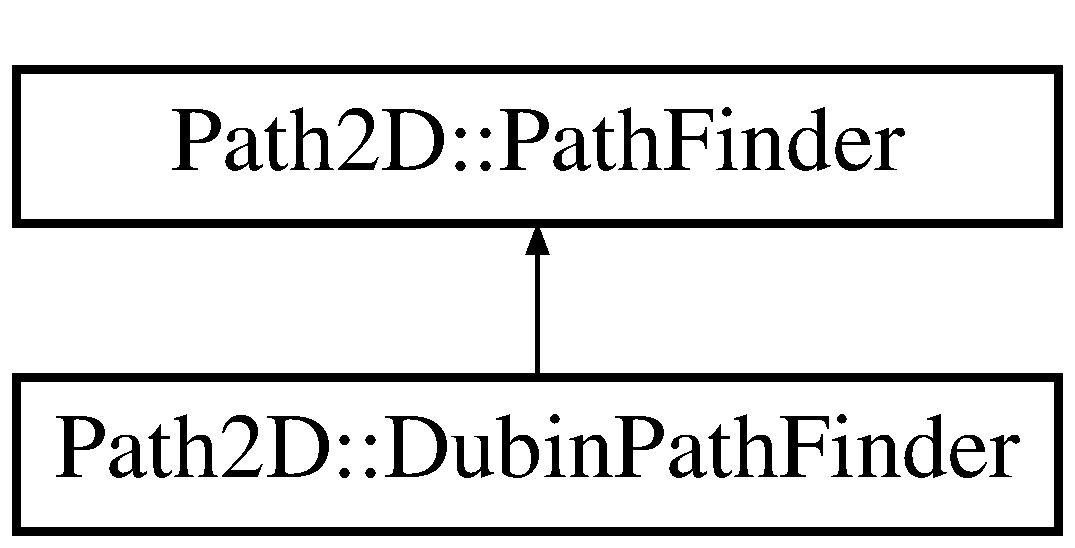
\includegraphics[height=2.000000cm]{class_path2_d_1_1_dubin_path_finder}
\end{center}
\end{figure}
\subsection*{Classes}
\begin{DoxyCompactItemize}
\item 
class \mbox{\hyperlink{class_path2_d_1_1_dubin_path_finder_1_1_possible_dubin_path}{Possible\+Dubin\+Path}}
\begin{DoxyCompactList}\small\item\em class that describes a possible dubin path (useful during the calculation) \end{DoxyCompactList}\item 
struct \mbox{\hyperlink{struct_path2_d_1_1_dubin_path_finder_1_1standard_conf}{standard\+Conf}}
\end{DoxyCompactItemize}
\subsection*{Public Member Functions}
\begin{DoxyCompactItemize}
\item 
\mbox{\hyperlink{class_path2_d_1_1_dubin_path_finder_a663ec1b97f56c4a36cbe242752d1253a}{Dubin\+Path\+Finder}} (\mbox{\hyperlink{class_path2_d_1_1_element_1_1_path_coordinates}{Path\+Coordinates}} path\+\_\+coordinates\+\_\+i, \mbox{\hyperlink{class_map}{Map}} $\ast$map\+\_\+i)
\begin{DoxyCompactList}\small\item\em constructor of the \mbox{\hyperlink{class_path2_d_1_1_dubin_path_finder}{Dubin\+Path\+Finder}} class \end{DoxyCompactList}\item 
\mbox{\Hypertarget{class_path2_d_1_1_dubin_path_finder_aa7bc3ba033b48ad8657e9c20b33c8f50}\label{class_path2_d_1_1_dubin_path_finder_aa7bc3ba033b48ad8657e9c20b33c8f50}} 
{\bfseries Dubin\+Path\+Finder} (\mbox{\hyperlink{class_map}{Map}} $\ast$map\+\_\+i)
\item 
\mbox{\Hypertarget{class_path2_d_1_1_dubin_path_finder_a053bc3ec20cfaf50927f055f2b0964d8}\label{class_path2_d_1_1_dubin_path_finder_a053bc3ec20cfaf50927f055f2b0964d8}} 
\mbox{\hyperlink{class_path2_d_1_1_dubin_path_finder_a053bc3ec20cfaf50927f055f2b0964d8}{$\sim$\+Dubin\+Path\+Finder}} ()
\begin{DoxyCompactList}\small\item\em destructor of the \mbox{\hyperlink{class_path2_d_1_1_dubin_path_finder}{Dubin\+Path\+Finder}} class \end{DoxyCompactList}\item 
std\+::vector$<$ \mbox{\hyperlink{class_path2_d_1_1_element_1_1_line}{Line}} $>$ \mbox{\hyperlink{class_path2_d_1_1_dubin_path_finder_abc1e93ad55c02aec66807fea41729ff6}{dubin\+Shortest\+Path}} (std\+::vector$<$ cv\+::\+Point $>$ \&alternative\+\_\+\+Points)
\begin{DoxyCompactList}\small\item\em function that find the dubins shortest path and return a vector of line \end{DoxyCompactList}\item 
std\+::vector$<$ \mbox{\hyperlink{class_path2_d_1_1_element_1_1_line}{Line}} $>$ \mbox{\hyperlink{class_path2_d_1_1_dubin_path_finder_a53d6ee86e364b403274f403af6e5088e}{shortest\+Path}} (std\+::vector$<$ cv\+::\+Point $>$ \&alternative\+\_\+\+Points)
\begin{DoxyCompactList}\small\item\em function that find the dubins shortest path and return a vector of line \end{DoxyCompactList}\end{DoxyCompactItemize}
\subsection*{Additional Inherited Members}


\subsection{Detailed Description}
Class that given the path coordinates allow to find the path using the dubins path algorithm. 

\subsection{Constructor \& Destructor Documentation}
\mbox{\Hypertarget{class_path2_d_1_1_dubin_path_finder_a663ec1b97f56c4a36cbe242752d1253a}\label{class_path2_d_1_1_dubin_path_finder_a663ec1b97f56c4a36cbe242752d1253a}} 
\index{Path2\+D\+::\+Dubin\+Path\+Finder@{Path2\+D\+::\+Dubin\+Path\+Finder}!Dubin\+Path\+Finder@{Dubin\+Path\+Finder}}
\index{Dubin\+Path\+Finder@{Dubin\+Path\+Finder}!Path2\+D\+::\+Dubin\+Path\+Finder@{Path2\+D\+::\+Dubin\+Path\+Finder}}
\subsubsection{\texorpdfstring{Dubin\+Path\+Finder()}{DubinPathFinder()}}
{\footnotesize\ttfamily Path2\+D\+::\+Dubin\+Path\+Finder\+::\+Dubin\+Path\+Finder (\begin{DoxyParamCaption}\item[{\mbox{\hyperlink{class_path2_d_1_1_element_1_1_path_coordinates}{Path\+Coordinates}}}]{path\+\_\+coordinates\+\_\+i,  }\item[{\mbox{\hyperlink{class_map}{Map}} $\ast$}]{map\+\_\+i }\end{DoxyParamCaption})}



constructor of the \mbox{\hyperlink{class_path2_d_1_1_dubin_path_finder}{Dubin\+Path\+Finder}} class 


\begin{DoxyParams}{Parameters}
{\em path\+\_\+coordinates\+\_\+i} & coordinates of the path that we want to find \\
\hline
\end{DoxyParams}


\subsection{Member Function Documentation}
\mbox{\Hypertarget{class_path2_d_1_1_dubin_path_finder_abc1e93ad55c02aec66807fea41729ff6}\label{class_path2_d_1_1_dubin_path_finder_abc1e93ad55c02aec66807fea41729ff6}} 
\index{Path2\+D\+::\+Dubin\+Path\+Finder@{Path2\+D\+::\+Dubin\+Path\+Finder}!dubin\+Shortest\+Path@{dubin\+Shortest\+Path}}
\index{dubin\+Shortest\+Path@{dubin\+Shortest\+Path}!Path2\+D\+::\+Dubin\+Path\+Finder@{Path2\+D\+::\+Dubin\+Path\+Finder}}
\subsubsection{\texorpdfstring{dubin\+Shortest\+Path()}{dubinShortestPath()}}
{\footnotesize\ttfamily std\+::vector$<$\mbox{\hyperlink{class_path2_d_1_1_element_1_1_line}{Line}}$>$ Path2\+D\+::\+Dubin\+Path\+Finder\+::dubin\+Shortest\+Path (\begin{DoxyParamCaption}\item[{std\+::vector$<$ cv\+::\+Point $>$ \&}]{alternative\+\_\+\+Points }\end{DoxyParamCaption})}



function that find the dubins shortest path and return a vector of line 

\begin{DoxyItemize}
\item alternative\+\_\+\+Points a point set for every obsticle that was found along the way \begin{DoxyReturn}{Returns}
vector of lines which describes the path 
\end{DoxyReturn}
\end{DoxyItemize}
\mbox{\Hypertarget{class_path2_d_1_1_dubin_path_finder_a53d6ee86e364b403274f403af6e5088e}\label{class_path2_d_1_1_dubin_path_finder_a53d6ee86e364b403274f403af6e5088e}} 
\index{Path2\+D\+::\+Dubin\+Path\+Finder@{Path2\+D\+::\+Dubin\+Path\+Finder}!shortest\+Path@{shortest\+Path}}
\index{shortest\+Path@{shortest\+Path}!Path2\+D\+::\+Dubin\+Path\+Finder@{Path2\+D\+::\+Dubin\+Path\+Finder}}
\subsubsection{\texorpdfstring{shortest\+Path()}{shortestPath()}}
{\footnotesize\ttfamily std\+::vector$<$\mbox{\hyperlink{class_path2_d_1_1_element_1_1_line}{Line}}$>$ Path2\+D\+::\+Dubin\+Path\+Finder\+::shortest\+Path (\begin{DoxyParamCaption}\item[{std\+::vector$<$ cv\+::\+Point $>$ \&}]{alternative\+\_\+\+Points }\end{DoxyParamCaption})\hspace{0.3cm}{\ttfamily [virtual]}}



function that find the dubins shortest path and return a vector of line 

\begin{DoxyItemize}
\item alternative\+\_\+\+Points a point set for every obsticle that was found along the way \begin{DoxyReturn}{Returns}
vector of lines which describes the path 
\end{DoxyReturn}
\end{DoxyItemize}


Implements \mbox{\hyperlink{class_path2_d_1_1_path_finder_a5d050326067c313925d87ac37612a181}{Path2\+D\+::\+Path\+Finder}}.



The documentation for this class was generated from the following file\+:\begin{DoxyCompactItemize}
\item 
Dubin\+Path\+Finder.\+hpp\end{DoxyCompactItemize}

\hypertarget{class_exit_point}{}\section{Exit\+Point Class Reference}
\label{class_exit_point}\index{Exit\+Point@{Exit\+Point}}


{\ttfamily \#include $<$Exit\+Point.\+hpp$>$}

Inheritance diagram for Exit\+Point\+:\begin{figure}[H]
\begin{center}
\leavevmode
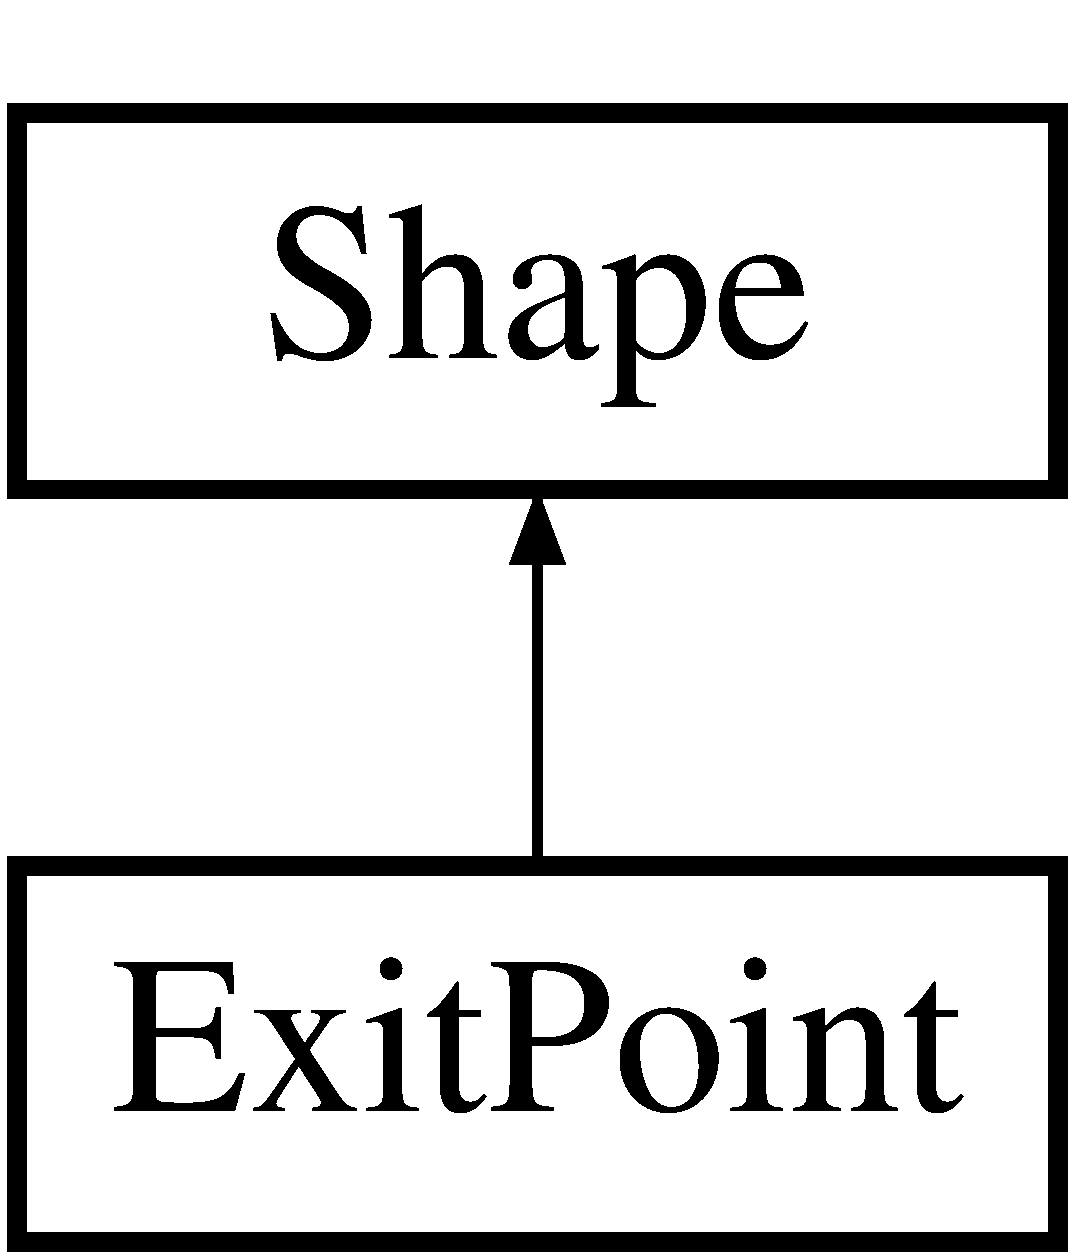
\includegraphics[height=2.000000cm]{class_exit_point}
\end{center}
\end{figure}
\subsection*{Public Member Functions}
\begin{DoxyCompactItemize}
\item 
\mbox{\hyperlink{class_exit_point_ae472f935e952356c9bfe64298474d523}{Exit\+Point}} ()
\item 
\mbox{\hyperlink{class_exit_point_aa764fee5b37cb7dbda6f2fde39ffbc05}{$\sim$\+Exit\+Point}} ()
\item 
void \mbox{\hyperlink{class_exit_point_a2762c0c61bbe71a1a292b86e9517e860}{find\+Exit\+Point}} (const Mat \&img)
\item 
std\+::vector$<$ cv\+::\+Point $>$ \mbox{\hyperlink{class_exit_point_ac26a595a35b370cf7375874395715af0}{get\+Corners}} ()
\item 
void \mbox{\hyperlink{class_exit_point_aff4341c31734d77224b1251988949430}{set\+Corners}} (std\+::vector$<$ cv\+::\+Point $>$ corners)
\item 
cv\+::\+Point \mbox{\hyperlink{class_exit_point_ad373de21603871832e10568631ef3cda}{get\+Top\+Left}} ()
\item 
void \mbox{\hyperlink{class_exit_point_a31c88803968c8b215062b97b699721e2}{set\+Top\+Left}} (cv\+::\+Point top\+Left)
\item 
cv\+::\+Point \mbox{\hyperlink{class_exit_point_a448716aa575ba751f72ab0f437b6a138}{get\+Top\+Right}} ()
\item 
void \mbox{\hyperlink{class_exit_point_ae27c395eb18321cb120b99ffbed6028a}{set\+Top\+Right}} (cv\+::\+Point top\+Right)
\item 
cv\+::\+Point \mbox{\hyperlink{class_exit_point_a51ac01267f39908e468ec859ba8d3096}{get\+Bottom\+Left}} ()
\item 
void \mbox{\hyperlink{class_exit_point_a22bf3a433b3567d36463699e16aaa86b}{set\+Bottom\+Left}} (cv\+::\+Point bottom\+Left)
\item 
cv\+::\+Point \mbox{\hyperlink{class_exit_point_a7a0e9d613aa361083bd4bf91f2080398}{get\+Bottom\+Right}} ()
\item 
void \mbox{\hyperlink{class_exit_point_afe10f2b0cf00b654dc1c95183462ed1a}{set\+Bottom\+Right}} (cv\+::\+Point bottom\+Right)
\end{DoxyCompactItemize}


\subsection{Detailed Description}
\mbox{\hyperlink{class_exit_point}{Exit\+Point}} class is able to detect and save the exit point given a photo 

\subsection{Constructor \& Destructor Documentation}
\mbox{\Hypertarget{class_exit_point_ae472f935e952356c9bfe64298474d523}\label{class_exit_point_ae472f935e952356c9bfe64298474d523}} 
\index{Exit\+Point@{Exit\+Point}!Exit\+Point@{Exit\+Point}}
\index{Exit\+Point@{Exit\+Point}!Exit\+Point@{Exit\+Point}}
\subsubsection{\texorpdfstring{Exit\+Point()}{ExitPoint()}}
{\footnotesize\ttfamily Exit\+Point\+::\+Exit\+Point (\begin{DoxyParamCaption}{ }\end{DoxyParamCaption})}

constructor of the \mbox{\hyperlink{class_exit_point}{Exit\+Point}} class \mbox{\Hypertarget{class_exit_point_aa764fee5b37cb7dbda6f2fde39ffbc05}\label{class_exit_point_aa764fee5b37cb7dbda6f2fde39ffbc05}} 
\index{Exit\+Point@{Exit\+Point}!````~Exit\+Point@{$\sim$\+Exit\+Point}}
\index{````~Exit\+Point@{$\sim$\+Exit\+Point}!Exit\+Point@{Exit\+Point}}
\subsubsection{\texorpdfstring{$\sim$\+Exit\+Point()}{~ExitPoint()}}
{\footnotesize\ttfamily Exit\+Point\+::$\sim$\+Exit\+Point (\begin{DoxyParamCaption}{ }\end{DoxyParamCaption})}

destructor of the \mbox{\hyperlink{class_exit_point}{Exit\+Point}} class 

\subsection{Member Function Documentation}
\mbox{\Hypertarget{class_exit_point_a2762c0c61bbe71a1a292b86e9517e860}\label{class_exit_point_a2762c0c61bbe71a1a292b86e9517e860}} 
\index{Exit\+Point@{Exit\+Point}!find\+Exit\+Point@{find\+Exit\+Point}}
\index{find\+Exit\+Point@{find\+Exit\+Point}!Exit\+Point@{Exit\+Point}}
\subsubsection{\texorpdfstring{find\+Exit\+Point()}{findExitPoint()}}
{\footnotesize\ttfamily void Exit\+Point\+::find\+Exit\+Point (\begin{DoxyParamCaption}\item[{const Mat \&}]{img }\end{DoxyParamCaption})}

retrieve and set the corners in the \mbox{\hyperlink{class_exit_point}{Exit\+Point}} object 
\begin{DoxyParams}{Parameters}
{\em img} & image of the arena \\
\hline
\end{DoxyParams}
\mbox{\Hypertarget{class_exit_point_a51ac01267f39908e468ec859ba8d3096}\label{class_exit_point_a51ac01267f39908e468ec859ba8d3096}} 
\index{Exit\+Point@{Exit\+Point}!get\+Bottom\+Left@{get\+Bottom\+Left}}
\index{get\+Bottom\+Left@{get\+Bottom\+Left}!Exit\+Point@{Exit\+Point}}
\subsubsection{\texorpdfstring{get\+Bottom\+Left()}{getBottomLeft()}}
{\footnotesize\ttfamily cv\+::\+Point Exit\+Point\+::get\+Bottom\+Left (\begin{DoxyParamCaption}{ }\end{DoxyParamCaption})}

return the bottom left corner \begin{DoxyReturn}{Returns}
the bottom left corner 
\end{DoxyReturn}
\mbox{\Hypertarget{class_exit_point_a7a0e9d613aa361083bd4bf91f2080398}\label{class_exit_point_a7a0e9d613aa361083bd4bf91f2080398}} 
\index{Exit\+Point@{Exit\+Point}!get\+Bottom\+Right@{get\+Bottom\+Right}}
\index{get\+Bottom\+Right@{get\+Bottom\+Right}!Exit\+Point@{Exit\+Point}}
\subsubsection{\texorpdfstring{get\+Bottom\+Right()}{getBottomRight()}}
{\footnotesize\ttfamily cv\+::\+Point Exit\+Point\+::get\+Bottom\+Right (\begin{DoxyParamCaption}{ }\end{DoxyParamCaption})}

return the bottom right corner of the exit point \begin{DoxyReturn}{Returns}
bottom right corner of the exit point 
\end{DoxyReturn}
\mbox{\Hypertarget{class_exit_point_ac26a595a35b370cf7375874395715af0}\label{class_exit_point_ac26a595a35b370cf7375874395715af0}} 
\index{Exit\+Point@{Exit\+Point}!get\+Corners@{get\+Corners}}
\index{get\+Corners@{get\+Corners}!Exit\+Point@{Exit\+Point}}
\subsubsection{\texorpdfstring{get\+Corners()}{getCorners()}}
{\footnotesize\ttfamily std\+::vector$<$cv\+::\+Point$>$ Exit\+Point\+::get\+Corners (\begin{DoxyParamCaption}{ }\end{DoxyParamCaption})}

return a list of corners in a clockwise order \begin{DoxyReturn}{Returns}
list of corners in a clockwise order 
\end{DoxyReturn}
\mbox{\Hypertarget{class_exit_point_ad373de21603871832e10568631ef3cda}\label{class_exit_point_ad373de21603871832e10568631ef3cda}} 
\index{Exit\+Point@{Exit\+Point}!get\+Top\+Left@{get\+Top\+Left}}
\index{get\+Top\+Left@{get\+Top\+Left}!Exit\+Point@{Exit\+Point}}
\subsubsection{\texorpdfstring{get\+Top\+Left()}{getTopLeft()}}
{\footnotesize\ttfamily cv\+::\+Point Exit\+Point\+::get\+Top\+Left (\begin{DoxyParamCaption}{ }\end{DoxyParamCaption})}

return the top left corner of the exit point \begin{DoxyReturn}{Returns}
return the top left corner of the exit point 
\end{DoxyReturn}
\mbox{\Hypertarget{class_exit_point_a448716aa575ba751f72ab0f437b6a138}\label{class_exit_point_a448716aa575ba751f72ab0f437b6a138}} 
\index{Exit\+Point@{Exit\+Point}!get\+Top\+Right@{get\+Top\+Right}}
\index{get\+Top\+Right@{get\+Top\+Right}!Exit\+Point@{Exit\+Point}}
\subsubsection{\texorpdfstring{get\+Top\+Right()}{getTopRight()}}
{\footnotesize\ttfamily cv\+::\+Point Exit\+Point\+::get\+Top\+Right (\begin{DoxyParamCaption}{ }\end{DoxyParamCaption})}

return the top right corner of the exit point \begin{DoxyReturn}{Returns}
return the top right corner of the exit point 
\end{DoxyReturn}
\mbox{\Hypertarget{class_exit_point_a22bf3a433b3567d36463699e16aaa86b}\label{class_exit_point_a22bf3a433b3567d36463699e16aaa86b}} 
\index{Exit\+Point@{Exit\+Point}!set\+Bottom\+Left@{set\+Bottom\+Left}}
\index{set\+Bottom\+Left@{set\+Bottom\+Left}!Exit\+Point@{Exit\+Point}}
\subsubsection{\texorpdfstring{set\+Bottom\+Left()}{setBottomLeft()}}
{\footnotesize\ttfamily void Exit\+Point\+::set\+Bottom\+Left (\begin{DoxyParamCaption}\item[{cv\+::\+Point}]{bottom\+Left }\end{DoxyParamCaption})}

set the bottom left corner 
\begin{DoxyParams}{Parameters}
{\em bottom\+Left} & bottom left corner of the exit point \\
\hline
\end{DoxyParams}
\mbox{\Hypertarget{class_exit_point_afe10f2b0cf00b654dc1c95183462ed1a}\label{class_exit_point_afe10f2b0cf00b654dc1c95183462ed1a}} 
\index{Exit\+Point@{Exit\+Point}!set\+Bottom\+Right@{set\+Bottom\+Right}}
\index{set\+Bottom\+Right@{set\+Bottom\+Right}!Exit\+Point@{Exit\+Point}}
\subsubsection{\texorpdfstring{set\+Bottom\+Right()}{setBottomRight()}}
{\footnotesize\ttfamily void Exit\+Point\+::set\+Bottom\+Right (\begin{DoxyParamCaption}\item[{cv\+::\+Point}]{bottom\+Right }\end{DoxyParamCaption})}

set the bottom right corner 
\begin{DoxyParams}{Parameters}
{\em bottom\+Right} & bottom right corner of the exit point \\
\hline
\end{DoxyParams}
\mbox{\Hypertarget{class_exit_point_aff4341c31734d77224b1251988949430}\label{class_exit_point_aff4341c31734d77224b1251988949430}} 
\index{Exit\+Point@{Exit\+Point}!set\+Corners@{set\+Corners}}
\index{set\+Corners@{set\+Corners}!Exit\+Point@{Exit\+Point}}
\subsubsection{\texorpdfstring{set\+Corners()}{setCorners()}}
{\footnotesize\ttfamily void Exit\+Point\+::set\+Corners (\begin{DoxyParamCaption}\item[{std\+::vector$<$ cv\+::\+Point $>$}]{corners }\end{DoxyParamCaption})}

set the list of corners 
\begin{DoxyParams}{Parameters}
{\em corners} & list of corners that have to be setted \\
\hline
\end{DoxyParams}
\mbox{\Hypertarget{class_exit_point_a31c88803968c8b215062b97b699721e2}\label{class_exit_point_a31c88803968c8b215062b97b699721e2}} 
\index{Exit\+Point@{Exit\+Point}!set\+Top\+Left@{set\+Top\+Left}}
\index{set\+Top\+Left@{set\+Top\+Left}!Exit\+Point@{Exit\+Point}}
\subsubsection{\texorpdfstring{set\+Top\+Left()}{setTopLeft()}}
{\footnotesize\ttfamily void Exit\+Point\+::set\+Top\+Left (\begin{DoxyParamCaption}\item[{cv\+::\+Point}]{top\+Left }\end{DoxyParamCaption})}

set the top left corner 
\begin{DoxyParams}{Parameters}
{\em top\+Left} & top left corner that has to be setted \\
\hline
\end{DoxyParams}
\mbox{\Hypertarget{class_exit_point_ae27c395eb18321cb120b99ffbed6028a}\label{class_exit_point_ae27c395eb18321cb120b99ffbed6028a}} 
\index{Exit\+Point@{Exit\+Point}!set\+Top\+Right@{set\+Top\+Right}}
\index{set\+Top\+Right@{set\+Top\+Right}!Exit\+Point@{Exit\+Point}}
\subsubsection{\texorpdfstring{set\+Top\+Right()}{setTopRight()}}
{\footnotesize\ttfamily void Exit\+Point\+::set\+Top\+Right (\begin{DoxyParamCaption}\item[{cv\+::\+Point}]{top\+Right }\end{DoxyParamCaption})}

set the top right corner 
\begin{DoxyParams}{Parameters}
{\em top\+Right} & top right corner tha has to be setted \\
\hline
\end{DoxyParams}


The documentation for this class was generated from the following file\+:\begin{DoxyCompactItemize}
\item 
Exit\+Point.\+hpp\end{DoxyCompactItemize}

\hypertarget{class_geometry2_d_1_1_hexagon}{}\section{Geometry2D\+:\+:Hexagon Class Reference}
\label{class_geometry2_d_1_1_hexagon}\index{Geometry2\+D\+::\+Hexagon@{Geometry2\+D\+::\+Hexagon}}


Class for handling hexagon obstacles.  




{\ttfamily \#include $<$Hexagon.\+hpp$>$}

Inheritance diagram for Geometry2D\+:\+:Hexagon\+:\begin{figure}[H]
\begin{center}
\leavevmode
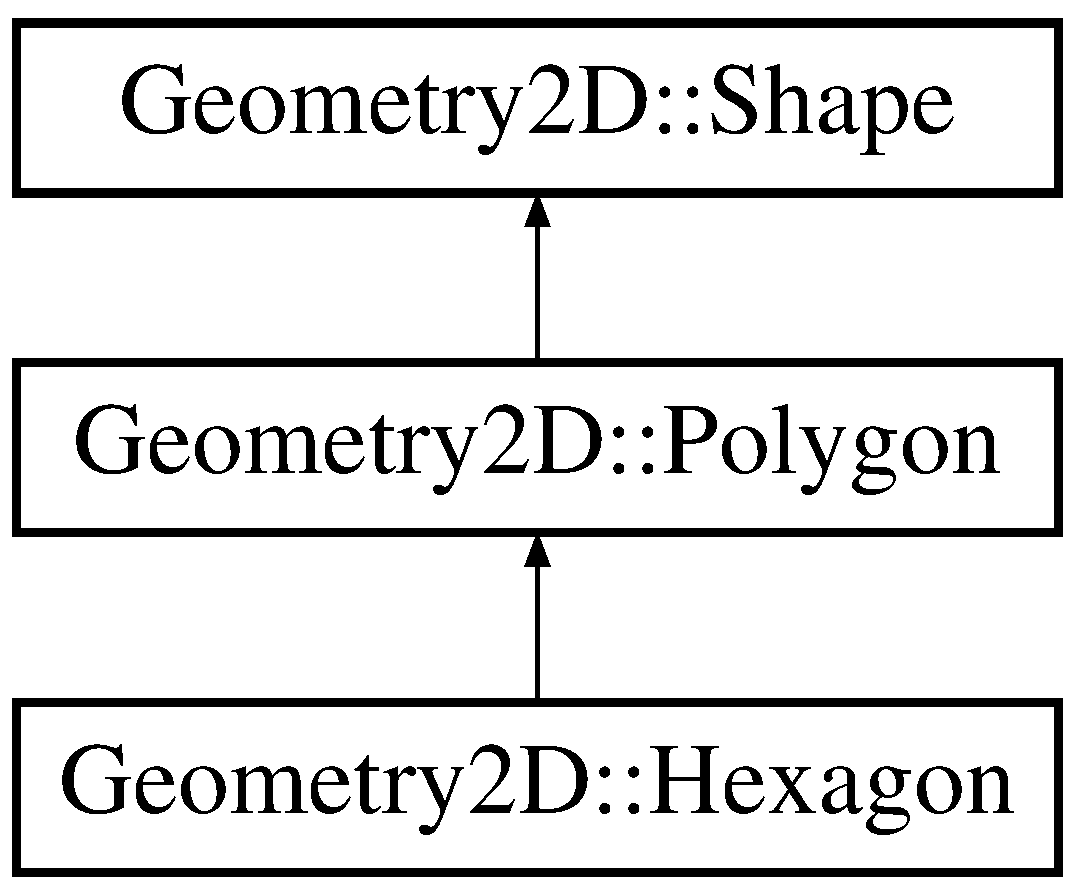
\includegraphics[height=3.000000cm]{class_geometry2_d_1_1_hexagon}
\end{center}
\end{figure}
\subsection*{Public Member Functions}
\begin{DoxyCompactItemize}
\item 
\mbox{\hyperlink{class_geometry2_d_1_1_hexagon_a5f151d8d0cb83ff62bb13196a0101a9e}{Hexagon}} ()
\item 
\mbox{\Hypertarget{class_geometry2_d_1_1_hexagon_add79e7752001e4c5c20e1a1e05672f56}\label{class_geometry2_d_1_1_hexagon_add79e7752001e4c5c20e1a1e05672f56}} 
{\bfseries Hexagon} (std\+::vector$<$ cv\+::\+Point $>$ \mbox{\hyperlink{class_geometry2_d_1_1_polygon_ab965e028324c2199022da00ff7eef14b}{points}})
\item 
\mbox{\hyperlink{class_geometry2_d_1_1_hexagon_aa16b14ea33395f3ec9ee58208c88eb1b}{$\sim$\+Hexagon}} ()
\item 
std\+::vector$<$ cv\+::\+Point $>$ \mbox{\hyperlink{class_geometry2_d_1_1_hexagon_ad72b9382bd173efc5aad346e7af074a0}{get\+Corners}} ()
\item 
void \mbox{\hyperlink{class_geometry2_d_1_1_hexagon_ab1557df2a9a0092e5cc23ff32f5f25bc}{set\+Corners}} (std\+::vector$<$ cv\+::\+Point $>$ corners)
\item 
\mbox{\Hypertarget{class_geometry2_d_1_1_hexagon_aa14a1979642db0e7a94ff0f9b59c7168}\label{class_geometry2_d_1_1_hexagon_aa14a1979642db0e7a94ff0f9b59c7168}} 
void \mbox{\hyperlink{class_geometry2_d_1_1_hexagon_aa14a1979642db0e7a94ff0f9b59c7168}{assign\+\_\+points}} ()
\begin{DoxyCompactList}\small\item\em assignes the points \end{DoxyCompactList}\end{DoxyCompactItemize}
\subsection*{Additional Inherited Members}


\subsection{Detailed Description}
Class for handling hexagon obstacles. 

\subsection{Constructor \& Destructor Documentation}
\mbox{\Hypertarget{class_geometry2_d_1_1_hexagon_a5f151d8d0cb83ff62bb13196a0101a9e}\label{class_geometry2_d_1_1_hexagon_a5f151d8d0cb83ff62bb13196a0101a9e}} 
\index{Geometry2\+D\+::\+Hexagon@{Geometry2\+D\+::\+Hexagon}!Hexagon@{Hexagon}}
\index{Hexagon@{Hexagon}!Geometry2\+D\+::\+Hexagon@{Geometry2\+D\+::\+Hexagon}}
\subsubsection{\texorpdfstring{Hexagon()}{Hexagon()}}
{\footnotesize\ttfamily Geometry2\+D\+::\+Hexagon\+::\+Hexagon (\begin{DoxyParamCaption}{ }\end{DoxyParamCaption})}

constructor of the \mbox{\hyperlink{class_geometry2_d_1_1_hexagon}{Hexagon}} class \mbox{\Hypertarget{class_geometry2_d_1_1_hexagon_aa16b14ea33395f3ec9ee58208c88eb1b}\label{class_geometry2_d_1_1_hexagon_aa16b14ea33395f3ec9ee58208c88eb1b}} 
\index{Geometry2\+D\+::\+Hexagon@{Geometry2\+D\+::\+Hexagon}!````~Hexagon@{$\sim$\+Hexagon}}
\index{````~Hexagon@{$\sim$\+Hexagon}!Geometry2\+D\+::\+Hexagon@{Geometry2\+D\+::\+Hexagon}}
\subsubsection{\texorpdfstring{$\sim$\+Hexagon()}{~Hexagon()}}
{\footnotesize\ttfamily Geometry2\+D\+::\+Hexagon\+::$\sim$\+Hexagon (\begin{DoxyParamCaption}{ }\end{DoxyParamCaption})}

destructor of the \mbox{\hyperlink{class_geometry2_d_1_1_hexagon}{Hexagon}} class 

\subsection{Member Function Documentation}
\mbox{\Hypertarget{class_geometry2_d_1_1_hexagon_ad72b9382bd173efc5aad346e7af074a0}\label{class_geometry2_d_1_1_hexagon_ad72b9382bd173efc5aad346e7af074a0}} 
\index{Geometry2\+D\+::\+Hexagon@{Geometry2\+D\+::\+Hexagon}!get\+Corners@{get\+Corners}}
\index{get\+Corners@{get\+Corners}!Geometry2\+D\+::\+Hexagon@{Geometry2\+D\+::\+Hexagon}}
\subsubsection{\texorpdfstring{get\+Corners()}{getCorners()}}
{\footnotesize\ttfamily std\+::vector$<$cv\+::\+Point$>$ Geometry2\+D\+::\+Hexagon\+::get\+Corners (\begin{DoxyParamCaption}{ }\end{DoxyParamCaption})}

return a list of corners of the hexagon \begin{DoxyReturn}{Returns}
list of corners of the hexagon 
\end{DoxyReturn}
\mbox{\Hypertarget{class_geometry2_d_1_1_hexagon_ab1557df2a9a0092e5cc23ff32f5f25bc}\label{class_geometry2_d_1_1_hexagon_ab1557df2a9a0092e5cc23ff32f5f25bc}} 
\index{Geometry2\+D\+::\+Hexagon@{Geometry2\+D\+::\+Hexagon}!set\+Corners@{set\+Corners}}
\index{set\+Corners@{set\+Corners}!Geometry2\+D\+::\+Hexagon@{Geometry2\+D\+::\+Hexagon}}
\subsubsection{\texorpdfstring{set\+Corners()}{setCorners()}}
{\footnotesize\ttfamily void Geometry2\+D\+::\+Hexagon\+::set\+Corners (\begin{DoxyParamCaption}\item[{std\+::vector$<$ cv\+::\+Point $>$}]{corners }\end{DoxyParamCaption})}

set the list of corners 
\begin{DoxyParams}{Parameters}
{\em corners} & list of corners \\
\hline
\end{DoxyParams}


The documentation for this class was generated from the following file\+:\begin{DoxyCompactItemize}
\item 
Hexagon.\+hpp\end{DoxyCompactItemize}

\hypertarget{struct_image_processing_1_1_h_s_v_filter_range}{}\section{Image\+Processing\+:\+:H\+S\+V\+Filter\+Range Struct Reference}
\label{struct_image_processing_1_1_h_s_v_filter_range}\index{Image\+Processing\+::\+H\+S\+V\+Filter\+Range@{Image\+Processing\+::\+H\+S\+V\+Filter\+Range}}


A structure that helps creating a color filter.  




{\ttfamily \#include $<$Color\+\_\+\+Processing.\+hpp$>$}

\subsection*{Public Member Functions}
\begin{DoxyCompactItemize}
\item 
\mbox{\Hypertarget{struct_image_processing_1_1_h_s_v_filter_range_a18e8316b637cccf1ad274e7d24bd30ff}\label{struct_image_processing_1_1_h_s_v_filter_range_a18e8316b637cccf1ad274e7d24bd30ff}} 
{\bfseries H\+S\+V\+Filter\+Range} (std\+::string quality)
\end{DoxyCompactItemize}
\subsection*{Public Attributes}
\begin{DoxyCompactItemize}
\item 
\mbox{\Hypertarget{struct_image_processing_1_1_h_s_v_filter_range_a739193d1bd8a9deb6bc3c1639add2156}\label{struct_image_processing_1_1_h_s_v_filter_range_a739193d1bd8a9deb6bc3c1639add2156}} 
cv\+::\+Scalar \mbox{\hyperlink{struct_image_processing_1_1_h_s_v_filter_range_a739193d1bd8a9deb6bc3c1639add2156}{ub}} = cv\+::\+Scalar(90, 255, 255)
\begin{DoxyCompactList}\small\item\em the upper bound of the filter \end{DoxyCompactList}\item 
\mbox{\Hypertarget{struct_image_processing_1_1_h_s_v_filter_range_abdd2bdaacd9ab1270b470e3913e0340e}\label{struct_image_processing_1_1_h_s_v_filter_range_abdd2bdaacd9ab1270b470e3913e0340e}} 
cv\+::\+Scalar \mbox{\hyperlink{struct_image_processing_1_1_h_s_v_filter_range_abdd2bdaacd9ab1270b470e3913e0340e}{lb}} = cv\+::\+Scalar(48, 53, 102)
\begin{DoxyCompactList}\small\item\em the lower bound of the filter \end{DoxyCompactList}\item 
\mbox{\Hypertarget{struct_image_processing_1_1_h_s_v_filter_range_a799a98eb547d036576f3d690ac25179f}\label{struct_image_processing_1_1_h_s_v_filter_range_a799a98eb547d036576f3d690ac25179f}} 
std\+::string \mbox{\hyperlink{struct_image_processing_1_1_h_s_v_filter_range_a799a98eb547d036576f3d690ac25179f}{saved\+\_\+quality}} = \char`\"{}bad\char`\"{}
\begin{DoxyCompactList}\small\item\em the saved tag \end{DoxyCompactList}\end{DoxyCompactItemize}


\subsection{Detailed Description}
A structure that helps creating a color filter. 

This structure contains several filter values for a given tag. It is able to store different values and dynamically change to another filter while keeping another filter in the back up. This allows the use of different filters to find a fitting one for a specific image 

The documentation for this struct was generated from the following file\+:\begin{DoxyCompactItemize}
\item 
Color\+\_\+\+Processing.\+hpp\end{DoxyCompactItemize}

\hypertarget{class_image_processing_1_1_inverse___perspective___mapping}{}\section{Image\+Processing\+:\+:Inverse\+\_\+\+Perspective\+\_\+\+Mapping Class Reference}
\label{class_image_processing_1_1_inverse___perspective___mapping}\index{Image\+Processing\+::\+Inverse\+\_\+\+Perspective\+\_\+\+Mapping@{Image\+Processing\+::\+Inverse\+\_\+\+Perspective\+\_\+\+Mapping}}


produce a perspective transformation around the arena given a photo  




{\ttfamily \#include $<$Inverse\+\_\+\+Perspective\+\_\+\+Mapping.\+hpp$>$}

\subsection*{Public Member Functions}
\begin{DoxyCompactItemize}
\item 
\mbox{\hyperlink{class_image_processing_1_1_inverse___perspective___mapping_a71da0ca3af64c1c8e0942040252ddf94}{Inverse\+\_\+\+Perspective\+\_\+\+Mapping}} ()
\item 
\mbox{\hyperlink{class_image_processing_1_1_inverse___perspective___mapping_afb34e6ac0791527427978ba4a373d555}{$\sim$\+Inverse\+\_\+\+Perspective\+\_\+\+Mapping}} ()
\item 
void \mbox{\hyperlink{class_image_processing_1_1_inverse___perspective___mapping_a7ba3059b10475460e490a3819df90469}{load\+Coefficients}} (const std\+::string \&filename, cv\+::\+Mat \&camera\+\_\+matrix, cv\+::\+Mat \&dist\+\_\+coeffs)
\item 
Mat \mbox{\hyperlink{class_image_processing_1_1_inverse___perspective___mapping_ac523ad6faeba3e5c87b9c1b6765866e4}{find\+Transform}} (const std\+::string \&calib\+\_\+image\+\_\+name, const cv\+::\+Mat \&camera\+\_\+matrix, const cv\+::\+Mat \&dist\+\_\+coeffs, double \&pixel\+\_\+scale, cv\+::\+Mat \&persp\+\_\+img)
\item 
void \mbox{\hyperlink{class_image_processing_1_1_inverse___perspective___mapping_ac97445de9425cb7e45c449dc33dfee6e}{store\+All\+Parameters}} (const std\+::string \&filename, const cv\+::\+Mat \&camera\+\_\+matrix, const cv\+::\+Mat \&dist\+\_\+coeffs, double pixel\+\_\+scale, const Mat \&persp\+\_\+transf)
\item 
cv\+::\+Mat \mbox{\hyperlink{class_image_processing_1_1_inverse___perspective___mapping_ab7cd3520a334dd38b26b93b385158c83}{run}} (std\+::string intrinsic\+\_\+conf, std\+::string image, std\+::string outputfilename)
\end{DoxyCompactItemize}


\subsection{Detailed Description}
produce a perspective transformation around the arena given a photo 

\subsection{Constructor \& Destructor Documentation}
\mbox{\Hypertarget{class_image_processing_1_1_inverse___perspective___mapping_a71da0ca3af64c1c8e0942040252ddf94}\label{class_image_processing_1_1_inverse___perspective___mapping_a71da0ca3af64c1c8e0942040252ddf94}} 
\index{Image\+Processing\+::\+Inverse\+\_\+\+Perspective\+\_\+\+Mapping@{Image\+Processing\+::\+Inverse\+\_\+\+Perspective\+\_\+\+Mapping}!Inverse\+\_\+\+Perspective\+\_\+\+Mapping@{Inverse\+\_\+\+Perspective\+\_\+\+Mapping}}
\index{Inverse\+\_\+\+Perspective\+\_\+\+Mapping@{Inverse\+\_\+\+Perspective\+\_\+\+Mapping}!Image\+Processing\+::\+Inverse\+\_\+\+Perspective\+\_\+\+Mapping@{Image\+Processing\+::\+Inverse\+\_\+\+Perspective\+\_\+\+Mapping}}
\subsubsection{\texorpdfstring{Inverse\+\_\+\+Perspective\+\_\+\+Mapping()}{Inverse\_Perspective\_Mapping()}}
{\footnotesize\ttfamily Image\+Processing\+::\+Inverse\+\_\+\+Perspective\+\_\+\+Mapping\+::\+Inverse\+\_\+\+Perspective\+\_\+\+Mapping (\begin{DoxyParamCaption}{ }\end{DoxyParamCaption})}

constructor of inverse perspective mapping class \mbox{\Hypertarget{class_image_processing_1_1_inverse___perspective___mapping_afb34e6ac0791527427978ba4a373d555}\label{class_image_processing_1_1_inverse___perspective___mapping_afb34e6ac0791527427978ba4a373d555}} 
\index{Image\+Processing\+::\+Inverse\+\_\+\+Perspective\+\_\+\+Mapping@{Image\+Processing\+::\+Inverse\+\_\+\+Perspective\+\_\+\+Mapping}!````~Inverse\+\_\+\+Perspective\+\_\+\+Mapping@{$\sim$\+Inverse\+\_\+\+Perspective\+\_\+\+Mapping}}
\index{````~Inverse\+\_\+\+Perspective\+\_\+\+Mapping@{$\sim$\+Inverse\+\_\+\+Perspective\+\_\+\+Mapping}!Image\+Processing\+::\+Inverse\+\_\+\+Perspective\+\_\+\+Mapping@{Image\+Processing\+::\+Inverse\+\_\+\+Perspective\+\_\+\+Mapping}}
\subsubsection{\texorpdfstring{$\sim$\+Inverse\+\_\+\+Perspective\+\_\+\+Mapping()}{~Inverse\_Perspective\_Mapping()}}
{\footnotesize\ttfamily Image\+Processing\+::\+Inverse\+\_\+\+Perspective\+\_\+\+Mapping\+::$\sim$\+Inverse\+\_\+\+Perspective\+\_\+\+Mapping (\begin{DoxyParamCaption}{ }\end{DoxyParamCaption})}

destructor of inverse perspective mapping class 

\subsection{Member Function Documentation}
\mbox{\Hypertarget{class_image_processing_1_1_inverse___perspective___mapping_ac523ad6faeba3e5c87b9c1b6765866e4}\label{class_image_processing_1_1_inverse___perspective___mapping_ac523ad6faeba3e5c87b9c1b6765866e4}} 
\index{Image\+Processing\+::\+Inverse\+\_\+\+Perspective\+\_\+\+Mapping@{Image\+Processing\+::\+Inverse\+\_\+\+Perspective\+\_\+\+Mapping}!find\+Transform@{find\+Transform}}
\index{find\+Transform@{find\+Transform}!Image\+Processing\+::\+Inverse\+\_\+\+Perspective\+\_\+\+Mapping@{Image\+Processing\+::\+Inverse\+\_\+\+Perspective\+\_\+\+Mapping}}
\subsubsection{\texorpdfstring{find\+Transform()}{findTransform()}}
{\footnotesize\ttfamily Mat Image\+Processing\+::\+Inverse\+\_\+\+Perspective\+\_\+\+Mapping\+::find\+Transform (\begin{DoxyParamCaption}\item[{const std\+::string \&}]{calib\+\_\+image\+\_\+name,  }\item[{const cv\+::\+Mat \&}]{camera\+\_\+matrix,  }\item[{const cv\+::\+Mat \&}]{dist\+\_\+coeffs,  }\item[{double \&}]{pixel\+\_\+scale,  }\item[{cv\+::\+Mat \&}]{persp\+\_\+img }\end{DoxyParamCaption})}

function to determine the perspective transformation of a rectangle on the ground plane 
\begin{DoxyParams}{Parameters}
{\em calib\+\_\+image\+\_\+name} & image \\
\hline
{\em camera\+\_\+matrix} & camera matrix \\
\hline
{\em dist\+\_\+coeffs} & distortion coefficents \\
\hline
{\em pixel\+\_\+scale} & pixel scaling \\
\hline
{\em persp\+\_\+img} & image after trasformation \\
\hline
\end{DoxyParams}
\begin{DoxyReturn}{Returns}

\end{DoxyReturn}
\mbox{\Hypertarget{class_image_processing_1_1_inverse___perspective___mapping_a7ba3059b10475460e490a3819df90469}\label{class_image_processing_1_1_inverse___perspective___mapping_a7ba3059b10475460e490a3819df90469}} 
\index{Image\+Processing\+::\+Inverse\+\_\+\+Perspective\+\_\+\+Mapping@{Image\+Processing\+::\+Inverse\+\_\+\+Perspective\+\_\+\+Mapping}!load\+Coefficients@{load\+Coefficients}}
\index{load\+Coefficients@{load\+Coefficients}!Image\+Processing\+::\+Inverse\+\_\+\+Perspective\+\_\+\+Mapping@{Image\+Processing\+::\+Inverse\+\_\+\+Perspective\+\_\+\+Mapping}}
\subsubsection{\texorpdfstring{load\+Coefficients()}{loadCoefficients()}}
{\footnotesize\ttfamily void Image\+Processing\+::\+Inverse\+\_\+\+Perspective\+\_\+\+Mapping\+::load\+Coefficients (\begin{DoxyParamCaption}\item[{const std\+::string \&}]{filename,  }\item[{cv\+::\+Mat \&}]{camera\+\_\+matrix,  }\item[{cv\+::\+Mat \&}]{dist\+\_\+coeffs }\end{DoxyParamCaption})}


\begin{DoxyParams}{Parameters}
{\em filename} & intrinsic calibration file name \\
\hline
{\em camera\+\_\+matrix} & camerat matrix file \\
\hline
{\em dist\+\_\+coeffs} & distortion coefficients \\
\hline
\end{DoxyParams}
\mbox{\Hypertarget{class_image_processing_1_1_inverse___perspective___mapping_ab7cd3520a334dd38b26b93b385158c83}\label{class_image_processing_1_1_inverse___perspective___mapping_ab7cd3520a334dd38b26b93b385158c83}} 
\index{Image\+Processing\+::\+Inverse\+\_\+\+Perspective\+\_\+\+Mapping@{Image\+Processing\+::\+Inverse\+\_\+\+Perspective\+\_\+\+Mapping}!run@{run}}
\index{run@{run}!Image\+Processing\+::\+Inverse\+\_\+\+Perspective\+\_\+\+Mapping@{Image\+Processing\+::\+Inverse\+\_\+\+Perspective\+\_\+\+Mapping}}
\subsubsection{\texorpdfstring{run()}{run()}}
{\footnotesize\ttfamily cv\+::\+Mat Image\+Processing\+::\+Inverse\+\_\+\+Perspective\+\_\+\+Mapping\+::run (\begin{DoxyParamCaption}\item[{std\+::string}]{intrinsic\+\_\+conf,  }\item[{std\+::string}]{image,  }\item[{std\+::string}]{outputfilename }\end{DoxyParamCaption})}

perform a perspective transformation 
\begin{DoxyParams}{Parameters}
{\em intrinsic\+\_\+conf} & \\
\hline
{\em image} & \\
\hline
{\em outputfilename} & \\
\hline
\end{DoxyParams}
\begin{DoxyReturn}{Returns}
the image after transformation 
\end{DoxyReturn}
\mbox{\Hypertarget{class_image_processing_1_1_inverse___perspective___mapping_ac97445de9425cb7e45c449dc33dfee6e}\label{class_image_processing_1_1_inverse___perspective___mapping_ac97445de9425cb7e45c449dc33dfee6e}} 
\index{Image\+Processing\+::\+Inverse\+\_\+\+Perspective\+\_\+\+Mapping@{Image\+Processing\+::\+Inverse\+\_\+\+Perspective\+\_\+\+Mapping}!store\+All\+Parameters@{store\+All\+Parameters}}
\index{store\+All\+Parameters@{store\+All\+Parameters}!Image\+Processing\+::\+Inverse\+\_\+\+Perspective\+\_\+\+Mapping@{Image\+Processing\+::\+Inverse\+\_\+\+Perspective\+\_\+\+Mapping}}
\subsubsection{\texorpdfstring{store\+All\+Parameters()}{storeAllParameters()}}
{\footnotesize\ttfamily void Image\+Processing\+::\+Inverse\+\_\+\+Perspective\+\_\+\+Mapping\+::store\+All\+Parameters (\begin{DoxyParamCaption}\item[{const std\+::string \&}]{filename,  }\item[{const cv\+::\+Mat \&}]{camera\+\_\+matrix,  }\item[{const cv\+::\+Mat \&}]{dist\+\_\+coeffs,  }\item[{double}]{pixel\+\_\+scale,  }\item[{const Mat \&}]{persp\+\_\+transf }\end{DoxyParamCaption})}

Store all the parameters to a file, for a later use, using the File\+Storage class methods 
\begin{DoxyParams}{Parameters}
{\em filename} & \\
\hline
{\em camera\+\_\+matrix} & \\
\hline
{\em dist\+\_\+coeffs} & \\
\hline
{\em pixel\+\_\+scale} & \\
\hline
{\em persp\+\_\+transf} & \\
\hline
\end{DoxyParams}


The documentation for this class was generated from the following file\+:\begin{DoxyCompactItemize}
\item 
Inverse\+\_\+\+Perspective\+\_\+\+Mapping.\+hpp\end{DoxyCompactItemize}

\hypertarget{class_path2_d_1_1_element_1_1_line}{}\section{Path2D\+:\+:Element\+:\+:Line Class Reference}
\label{class_path2_d_1_1_element_1_1_line}\index{Path2\+D\+::\+Element\+::\+Line@{Path2\+D\+::\+Element\+::\+Line}}


\mbox{\hyperlink{class_path2_d_1_1_element_1_1_line}{Line}} class that describes the basic line of a path.  




{\ttfamily \#include $<$Line.\+hpp$>$}

Inheritance diagram for Path2D\+:\+:Element\+:\+:Line\+:\begin{figure}[H]
\begin{center}
\leavevmode
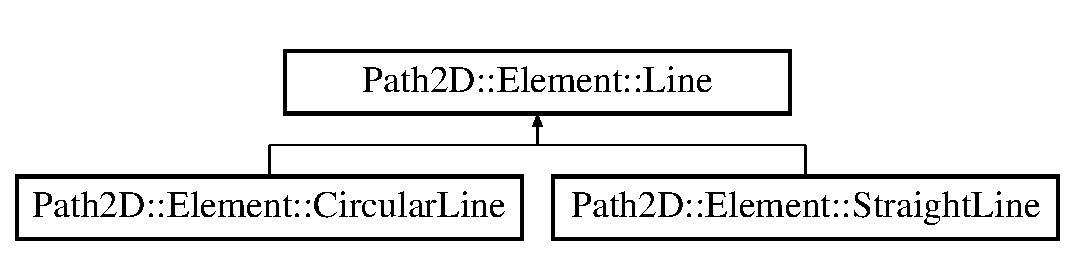
\includegraphics[height=2.000000cm]{class_path2_d_1_1_element_1_1_line}
\end{center}
\end{figure}
\subsection*{Public Member Functions}
\begin{DoxyCompactItemize}
\item 
\mbox{\Hypertarget{class_path2_d_1_1_element_1_1_line_a994412817c823da52472fb49f58a00f7}\label{class_path2_d_1_1_element_1_1_line_a994412817c823da52472fb49f58a00f7}} 
\mbox{\hyperlink{class_path2_d_1_1_element_1_1_line_a994412817c823da52472fb49f58a00f7}{Line}} ()
\begin{DoxyCompactList}\small\item\em constructor of \mbox{\hyperlink{class_path2_d_1_1_element_1_1_line}{Line}} class \end{DoxyCompactList}\item 
\mbox{\hyperlink{class_path2_d_1_1_element_1_1_line_a88244ad1861298c071c3f63b6726fad2}{Line}} (\mbox{\hyperlink{class_path2_d_1_1_element_1_1_position}{Position}} start\+\_\+point, \mbox{\hyperlink{class_path2_d_1_1_element_1_1_position}{Position}} end\+\_\+point)
\begin{DoxyCompactList}\small\item\em contrusctor of \mbox{\hyperlink{class_path2_d_1_1_element_1_1_line}{Line}} class \end{DoxyCompactList}\item 
\mbox{\Hypertarget{class_path2_d_1_1_element_1_1_line_a82f0610f7a03d00f3560765b93cf9435}\label{class_path2_d_1_1_element_1_1_line_a82f0610f7a03d00f3560765b93cf9435}} 
\mbox{\hyperlink{class_path2_d_1_1_element_1_1_line_a82f0610f7a03d00f3560765b93cf9435}{$\sim$\+Line}} ()
\begin{DoxyCompactList}\small\item\em destructor of the line path \end{DoxyCompactList}\item 
void \mbox{\hyperlink{class_path2_d_1_1_element_1_1_line_a942a5789b98659054b06c2c1a99b9c4d}{set\+Start\+Point}} (\mbox{\hyperlink{class_path2_d_1_1_element_1_1_position}{Position}} start\+\_\+point\+\_\+i)
\begin{DoxyCompactList}\small\item\em set the start position of the path \end{DoxyCompactList}\item 
\mbox{\hyperlink{class_path2_d_1_1_element_1_1_position}{Position}} \mbox{\hyperlink{class_path2_d_1_1_element_1_1_line_a1170a26baad8c08c33b1eecbb0305810}{get\+Start\+Point}} ()
\begin{DoxyCompactList}\small\item\em return the start point of the path \end{DoxyCompactList}\item 
void \mbox{\hyperlink{class_path2_d_1_1_element_1_1_line_a39675d1b58137465633f037aabfb57cc}{set\+End\+Point}} (\mbox{\hyperlink{class_path2_d_1_1_element_1_1_position}{Position}} end\+\_\+point\+\_\+i)
\begin{DoxyCompactList}\small\item\em set the end point of the path \end{DoxyCompactList}\item 
\mbox{\hyperlink{class_path2_d_1_1_element_1_1_position}{Position}} \mbox{\hyperlink{class_path2_d_1_1_element_1_1_line_ac0812b487cf344441073a9a49ee1b82d}{get\+End\+Point}} ()
\begin{DoxyCompactList}\small\item\em return the end point of the path \end{DoxyCompactList}\item 
void \mbox{\hyperlink{class_path2_d_1_1_element_1_1_line_ac18f28815c521092a2b1930647fae171}{set\+Length}} (double length\+\_\+i)
\begin{DoxyCompactList}\small\item\em set the length of the path \end{DoxyCompactList}\item 
double \mbox{\hyperlink{class_path2_d_1_1_element_1_1_line_a9f75579914f368af881348c298ecefb1}{get\+Length}} ()
\item 
\mbox{\hyperlink{class_path2_d_1_1_element_1_1_position}{Position}} \mbox{\hyperlink{class_path2_d_1_1_element_1_1_line_a375516699c55aee53a48ba9c3e819da8}{find\+Point\+Distance}} (double k, \mbox{\hyperlink{class_path2_d_1_1_element_1_1_position}{Position}} start, double length)
\begin{DoxyCompactList}\small\item\em function that given the curvature the start point and the lenght of the path allow to find the end point of the line \end{DoxyCompactList}\item 
double \mbox{\hyperlink{class_path2_d_1_1_element_1_1_line_a3ab3acf1cc03a38c0f9365edcf5088ab}{sinc}} (double inp)
\begin{DoxyCompactList}\small\item\em Implementation of function sinc(t), returning 1 for t==0, and sin(t)/t. \end{DoxyCompactList}\item 
double \mbox{\hyperlink{class_path2_d_1_1_element_1_1_line_acf0f091fc601933343d71f166932e109}{mod2pi}} (double ang)
\begin{DoxyCompactList}\small\item\em Normalize an angle (in range \mbox{[}0,2$\ast$pi)) \end{DoxyCompactList}\item 
\mbox{\Hypertarget{class_path2_d_1_1_element_1_1_line_ad2ca1d21a7917a57340813ad742bd81d}\label{class_path2_d_1_1_element_1_1_line_ad2ca1d21a7917a57340813ad742bd81d}} 
void \mbox{\hyperlink{class_path2_d_1_1_element_1_1_line_ad2ca1d21a7917a57340813ad742bd81d}{set\+Curvature}} (double curvature\+\_\+i)
\begin{DoxyCompactList}\small\item\em allow to set the curvature of the line \end{DoxyCompactList}\item 
double \mbox{\hyperlink{class_path2_d_1_1_element_1_1_line_a837b53f6b6604ddbd40b16842897961b}{get\+Curvature}} ()
\item 
\mbox{\Hypertarget{class_path2_d_1_1_element_1_1_line_a61f99c8af2a6c1bc08653159df510f0f}\label{class_path2_d_1_1_element_1_1_line_a61f99c8af2a6c1bc08653159df510f0f}} 
void {\bfseries set\+Intermediate\+Points} (std\+::vector$<$ Point2d $>$ \&intermediate\+\_\+points)
\item 
\mbox{\Hypertarget{class_path2_d_1_1_element_1_1_line_a455a0a414cee38680e06433247e6fa01}\label{class_path2_d_1_1_element_1_1_line_a455a0a414cee38680e06433247e6fa01}} 
std\+::vector$<$ Point2d $>$ {\bfseries get\+Intermediate\+Points} ()
\end{DoxyCompactItemize}


\subsection{Detailed Description}
\mbox{\hyperlink{class_path2_d_1_1_element_1_1_line}{Line}} class that describes the basic line of a path. 

\subsection{Constructor \& Destructor Documentation}
\mbox{\Hypertarget{class_path2_d_1_1_element_1_1_line_a88244ad1861298c071c3f63b6726fad2}\label{class_path2_d_1_1_element_1_1_line_a88244ad1861298c071c3f63b6726fad2}} 
\index{Path2\+D\+::\+Element\+::\+Line@{Path2\+D\+::\+Element\+::\+Line}!Line@{Line}}
\index{Line@{Line}!Path2\+D\+::\+Element\+::\+Line@{Path2\+D\+::\+Element\+::\+Line}}
\subsubsection{\texorpdfstring{Line()}{Line()}}
{\footnotesize\ttfamily Path2\+D\+::\+Element\+::\+Line\+::\+Line (\begin{DoxyParamCaption}\item[{\mbox{\hyperlink{class_path2_d_1_1_element_1_1_position}{Position}}}]{start\+\_\+point,  }\item[{\mbox{\hyperlink{class_path2_d_1_1_element_1_1_position}{Position}}}]{end\+\_\+point }\end{DoxyParamCaption})}



contrusctor of \mbox{\hyperlink{class_path2_d_1_1_element_1_1_line}{Line}} class 


\begin{DoxyParams}{Parameters}
{\em start\+\_\+point} & start point of the path \\
\hline
{\em end\+\_\+point} & end point of the path \\
\hline
\end{DoxyParams}


\subsection{Member Function Documentation}
\mbox{\Hypertarget{class_path2_d_1_1_element_1_1_line_a375516699c55aee53a48ba9c3e819da8}\label{class_path2_d_1_1_element_1_1_line_a375516699c55aee53a48ba9c3e819da8}} 
\index{Path2\+D\+::\+Element\+::\+Line@{Path2\+D\+::\+Element\+::\+Line}!find\+Point\+Distance@{find\+Point\+Distance}}
\index{find\+Point\+Distance@{find\+Point\+Distance}!Path2\+D\+::\+Element\+::\+Line@{Path2\+D\+::\+Element\+::\+Line}}
\subsubsection{\texorpdfstring{find\+Point\+Distance()}{findPointDistance()}}
{\footnotesize\ttfamily \mbox{\hyperlink{class_path2_d_1_1_element_1_1_position}{Position}} Path2\+D\+::\+Element\+::\+Line\+::find\+Point\+Distance (\begin{DoxyParamCaption}\item[{double}]{k,  }\item[{\mbox{\hyperlink{class_path2_d_1_1_element_1_1_position}{Position}}}]{start,  }\item[{double}]{length }\end{DoxyParamCaption})}



function that given the curvature the start point and the lenght of the path allow to find the end point of the line 


\begin{DoxyParams}{Parameters}
{\em k} & curvature \\
\hline
{\em start} & start point of the line \\
\hline
{\em length} & length of the line \\
\hline
\end{DoxyParams}
\begin{DoxyReturn}{Returns}

\end{DoxyReturn}
\mbox{\Hypertarget{class_path2_d_1_1_element_1_1_line_a837b53f6b6604ddbd40b16842897961b}\label{class_path2_d_1_1_element_1_1_line_a837b53f6b6604ddbd40b16842897961b}} 
\index{Path2\+D\+::\+Element\+::\+Line@{Path2\+D\+::\+Element\+::\+Line}!get\+Curvature@{get\+Curvature}}
\index{get\+Curvature@{get\+Curvature}!Path2\+D\+::\+Element\+::\+Line@{Path2\+D\+::\+Element\+::\+Line}}
\subsubsection{\texorpdfstring{get\+Curvature()}{getCurvature()}}
{\footnotesize\ttfamily double Path2\+D\+::\+Element\+::\+Line\+::get\+Curvature (\begin{DoxyParamCaption}{ }\end{DoxyParamCaption})}

return the curvature of the line \begin{DoxyReturn}{Returns}
curvature of the line 
\end{DoxyReturn}
\mbox{\Hypertarget{class_path2_d_1_1_element_1_1_line_ac0812b487cf344441073a9a49ee1b82d}\label{class_path2_d_1_1_element_1_1_line_ac0812b487cf344441073a9a49ee1b82d}} 
\index{Path2\+D\+::\+Element\+::\+Line@{Path2\+D\+::\+Element\+::\+Line}!get\+End\+Point@{get\+End\+Point}}
\index{get\+End\+Point@{get\+End\+Point}!Path2\+D\+::\+Element\+::\+Line@{Path2\+D\+::\+Element\+::\+Line}}
\subsubsection{\texorpdfstring{get\+End\+Point()}{getEndPoint()}}
{\footnotesize\ttfamily \mbox{\hyperlink{class_path2_d_1_1_element_1_1_position}{Position}} Path2\+D\+::\+Element\+::\+Line\+::get\+End\+Point (\begin{DoxyParamCaption}{ }\end{DoxyParamCaption})}



return the end point of the path 

\begin{DoxyReturn}{Returns}
the end point of the path 
\end{DoxyReturn}
\mbox{\Hypertarget{class_path2_d_1_1_element_1_1_line_a9f75579914f368af881348c298ecefb1}\label{class_path2_d_1_1_element_1_1_line_a9f75579914f368af881348c298ecefb1}} 
\index{Path2\+D\+::\+Element\+::\+Line@{Path2\+D\+::\+Element\+::\+Line}!get\+Length@{get\+Length}}
\index{get\+Length@{get\+Length}!Path2\+D\+::\+Element\+::\+Line@{Path2\+D\+::\+Element\+::\+Line}}
\subsubsection{\texorpdfstring{get\+Length()}{getLength()}}
{\footnotesize\ttfamily double Path2\+D\+::\+Element\+::\+Line\+::get\+Length (\begin{DoxyParamCaption}{ }\end{DoxyParamCaption})}

return the length of the path \begin{DoxyReturn}{Returns}
the length of the path 
\end{DoxyReturn}
\mbox{\Hypertarget{class_path2_d_1_1_element_1_1_line_a1170a26baad8c08c33b1eecbb0305810}\label{class_path2_d_1_1_element_1_1_line_a1170a26baad8c08c33b1eecbb0305810}} 
\index{Path2\+D\+::\+Element\+::\+Line@{Path2\+D\+::\+Element\+::\+Line}!get\+Start\+Point@{get\+Start\+Point}}
\index{get\+Start\+Point@{get\+Start\+Point}!Path2\+D\+::\+Element\+::\+Line@{Path2\+D\+::\+Element\+::\+Line}}
\subsubsection{\texorpdfstring{get\+Start\+Point()}{getStartPoint()}}
{\footnotesize\ttfamily \mbox{\hyperlink{class_path2_d_1_1_element_1_1_position}{Position}} Path2\+D\+::\+Element\+::\+Line\+::get\+Start\+Point (\begin{DoxyParamCaption}{ }\end{DoxyParamCaption})}



return the start point of the path 

\begin{DoxyReturn}{Returns}
the start point 
\end{DoxyReturn}
\mbox{\Hypertarget{class_path2_d_1_1_element_1_1_line_acf0f091fc601933343d71f166932e109}\label{class_path2_d_1_1_element_1_1_line_acf0f091fc601933343d71f166932e109}} 
\index{Path2\+D\+::\+Element\+::\+Line@{Path2\+D\+::\+Element\+::\+Line}!mod2pi@{mod2pi}}
\index{mod2pi@{mod2pi}!Path2\+D\+::\+Element\+::\+Line@{Path2\+D\+::\+Element\+::\+Line}}
\subsubsection{\texorpdfstring{mod2pi()}{mod2pi()}}
{\footnotesize\ttfamily double Path2\+D\+::\+Element\+::\+Line\+::mod2pi (\begin{DoxyParamCaption}\item[{double}]{ang }\end{DoxyParamCaption})}



Normalize an angle (in range \mbox{[}0,2$\ast$pi)) 


\begin{DoxyParams}{Parameters}
{\em ang} & input angle \\
\hline
\end{DoxyParams}
\begin{DoxyReturn}{Returns}
the normalize angle in range \mbox{[}0,2$\ast$pi\mbox{]} 
\end{DoxyReturn}
\mbox{\Hypertarget{class_path2_d_1_1_element_1_1_line_a39675d1b58137465633f037aabfb57cc}\label{class_path2_d_1_1_element_1_1_line_a39675d1b58137465633f037aabfb57cc}} 
\index{Path2\+D\+::\+Element\+::\+Line@{Path2\+D\+::\+Element\+::\+Line}!set\+End\+Point@{set\+End\+Point}}
\index{set\+End\+Point@{set\+End\+Point}!Path2\+D\+::\+Element\+::\+Line@{Path2\+D\+::\+Element\+::\+Line}}
\subsubsection{\texorpdfstring{set\+End\+Point()}{setEndPoint()}}
{\footnotesize\ttfamily void Path2\+D\+::\+Element\+::\+Line\+::set\+End\+Point (\begin{DoxyParamCaption}\item[{\mbox{\hyperlink{class_path2_d_1_1_element_1_1_position}{Position}}}]{end\+\_\+point\+\_\+i }\end{DoxyParamCaption})}



set the end point of the path 


\begin{DoxyParams}{Parameters}
{\em end\+\_\+point\+\_\+i} & the end point of the path \\
\hline
\end{DoxyParams}
\mbox{\Hypertarget{class_path2_d_1_1_element_1_1_line_ac18f28815c521092a2b1930647fae171}\label{class_path2_d_1_1_element_1_1_line_ac18f28815c521092a2b1930647fae171}} 
\index{Path2\+D\+::\+Element\+::\+Line@{Path2\+D\+::\+Element\+::\+Line}!set\+Length@{set\+Length}}
\index{set\+Length@{set\+Length}!Path2\+D\+::\+Element\+::\+Line@{Path2\+D\+::\+Element\+::\+Line}}
\subsubsection{\texorpdfstring{set\+Length()}{setLength()}}
{\footnotesize\ttfamily void Path2\+D\+::\+Element\+::\+Line\+::set\+Length (\begin{DoxyParamCaption}\item[{double}]{length\+\_\+i }\end{DoxyParamCaption})}



set the length of the path 


\begin{DoxyParams}{Parameters}
{\em length\+\_\+i} & the length of the path \\
\hline
\end{DoxyParams}
\mbox{\Hypertarget{class_path2_d_1_1_element_1_1_line_a942a5789b98659054b06c2c1a99b9c4d}\label{class_path2_d_1_1_element_1_1_line_a942a5789b98659054b06c2c1a99b9c4d}} 
\index{Path2\+D\+::\+Element\+::\+Line@{Path2\+D\+::\+Element\+::\+Line}!set\+Start\+Point@{set\+Start\+Point}}
\index{set\+Start\+Point@{set\+Start\+Point}!Path2\+D\+::\+Element\+::\+Line@{Path2\+D\+::\+Element\+::\+Line}}
\subsubsection{\texorpdfstring{set\+Start\+Point()}{setStartPoint()}}
{\footnotesize\ttfamily void Path2\+D\+::\+Element\+::\+Line\+::set\+Start\+Point (\begin{DoxyParamCaption}\item[{\mbox{\hyperlink{class_path2_d_1_1_element_1_1_position}{Position}}}]{start\+\_\+point\+\_\+i }\end{DoxyParamCaption})}



set the start position of the path 


\begin{DoxyParams}{Parameters}
{\em start\+\_\+point\+\_\+i} & start point of the path \\
\hline
\end{DoxyParams}
\mbox{\Hypertarget{class_path2_d_1_1_element_1_1_line_a3ab3acf1cc03a38c0f9365edcf5088ab}\label{class_path2_d_1_1_element_1_1_line_a3ab3acf1cc03a38c0f9365edcf5088ab}} 
\index{Path2\+D\+::\+Element\+::\+Line@{Path2\+D\+::\+Element\+::\+Line}!sinc@{sinc}}
\index{sinc@{sinc}!Path2\+D\+::\+Element\+::\+Line@{Path2\+D\+::\+Element\+::\+Line}}
\subsubsection{\texorpdfstring{sinc()}{sinc()}}
{\footnotesize\ttfamily double Path2\+D\+::\+Element\+::\+Line\+::sinc (\begin{DoxyParamCaption}\item[{double}]{inp }\end{DoxyParamCaption})}



Implementation of function sinc(t), returning 1 for t==0, and sin(t)/t. 


\begin{DoxyParams}{Parameters}
{\em inp} & input angle \\
\hline
\end{DoxyParams}
\begin{DoxyReturn}{Returns}
1 for inp==0 otherwise sin(inp)/inp 
\end{DoxyReturn}


The documentation for this class was generated from the following file\+:\begin{DoxyCompactItemize}
\item 
Line.\+hpp\end{DoxyCompactItemize}

\hypertarget{class_map}{}\section{Map Class Reference}
\label{class_map}\index{Map@{Map}}
\subsection*{Public Member Functions}
\begin{DoxyCompactItemize}
\item 
\mbox{\Hypertarget{class_map_a02537656e91e97077dfdfc5d84c3027b}\label{class_map_a02537656e91e97077dfdfc5d84c3027b}} 
void {\bfseries create\+Map} (const Mat \&img)
\end{DoxyCompactItemize}


The documentation for this class was generated from the following file\+:\begin{DoxyCompactItemize}
\item 
Map.\+hpp\end{DoxyCompactItemize}

\hypertarget{class_obstacle}{}\section{Obstacle Class Reference}
\label{class_obstacle}\index{Obstacle@{Obstacle}}


class for handling obstacles in the map  




{\ttfamily \#include $<$Obstacle.\+hpp$>$}

Inheritance diagram for Obstacle\+:\begin{figure}[H]
\begin{center}
\leavevmode
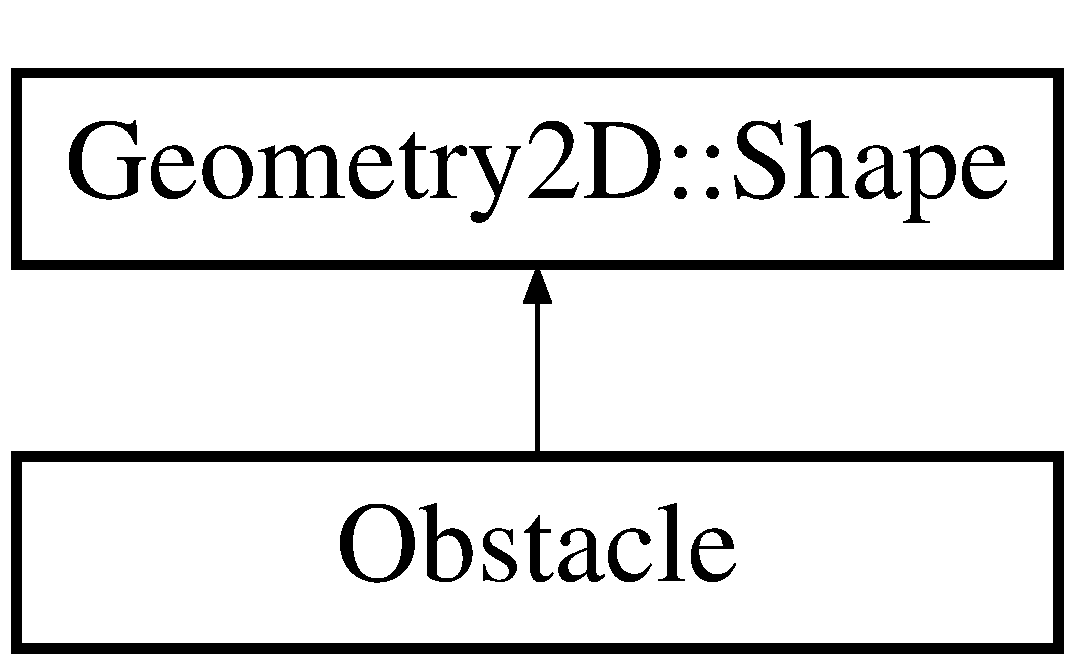
\includegraphics[height=2.000000cm]{class_obstacle}
\end{center}
\end{figure}
\subsection*{Public Member Functions}
\begin{DoxyCompactItemize}
\item 
\mbox{\hyperlink{class_obstacle_a8f734072321fa06a7b7dae2d5f50f352}{Obstacle}} ()
\item 
\mbox{\hyperlink{class_obstacle_af2f9cc9c6cff75dca0974fd5ac4f71a9}{$\sim$\+Obstacle}} ()
\item 
void \mbox{\hyperlink{class_obstacle_ae333b23b742b38e50be13bc7aec2da5b}{find\+Obstacles}} (const Mat \&img)
\item 
std\+::vector$<$ \mbox{\hyperlink{class_geometry2_d_1_1_triangle}{Triangle}} $\ast$ $>$ \mbox{\hyperlink{class_obstacle_ae4541d52e558b0995203e99d09d4d5d6}{get\+Triangles}} ()
\item 
std\+::vector$<$ \mbox{\hyperlink{class_geometry2_d_1_1_square}{Square}} $\ast$ $>$ \mbox{\hyperlink{class_obstacle_aa7d4a88d87f53bc8ba1e2b9123354f3c}{get\+Squares}} ()
\item 
std\+::vector$<$ \mbox{\hyperlink{class_geometry2_d_1_1_pentagon}{Pentagon}} $\ast$ $>$ \mbox{\hyperlink{class_obstacle_a7cbf1671e8fef324fe113517094f8428}{get\+Pentagons}} ()
\item 
std\+::vector$<$ \mbox{\hyperlink{class_geometry2_d_1_1_hexagon}{Hexagon}} $\ast$ $>$ \mbox{\hyperlink{class_obstacle_a26db0857f78a85a975957720eeb0464d}{get\+Hexagons}} ()
\end{DoxyCompactItemize}


\subsection{Detailed Description}
class for handling obstacles in the map 

\subsection{Constructor \& Destructor Documentation}
\mbox{\Hypertarget{class_obstacle_a8f734072321fa06a7b7dae2d5f50f352}\label{class_obstacle_a8f734072321fa06a7b7dae2d5f50f352}} 
\index{Obstacle@{Obstacle}!Obstacle@{Obstacle}}
\index{Obstacle@{Obstacle}!Obstacle@{Obstacle}}
\subsubsection{\texorpdfstring{Obstacle()}{Obstacle()}}
{\footnotesize\ttfamily Obstacle\+::\+Obstacle (\begin{DoxyParamCaption}{ }\end{DoxyParamCaption})}

contstructor of the \mbox{\hyperlink{class_obstacle}{Obstacle}} class \mbox{\Hypertarget{class_obstacle_af2f9cc9c6cff75dca0974fd5ac4f71a9}\label{class_obstacle_af2f9cc9c6cff75dca0974fd5ac4f71a9}} 
\index{Obstacle@{Obstacle}!````~Obstacle@{$\sim$\+Obstacle}}
\index{````~Obstacle@{$\sim$\+Obstacle}!Obstacle@{Obstacle}}
\subsubsection{\texorpdfstring{$\sim$\+Obstacle()}{~Obstacle()}}
{\footnotesize\ttfamily Obstacle\+::$\sim$\+Obstacle (\begin{DoxyParamCaption}{ }\end{DoxyParamCaption})}

destructor of the \mbox{\hyperlink{class_obstacle}{Obstacle}} class 

\subsection{Member Function Documentation}
\mbox{\Hypertarget{class_obstacle_ae333b23b742b38e50be13bc7aec2da5b}\label{class_obstacle_ae333b23b742b38e50be13bc7aec2da5b}} 
\index{Obstacle@{Obstacle}!find\+Obstacles@{find\+Obstacles}}
\index{find\+Obstacles@{find\+Obstacles}!Obstacle@{Obstacle}}
\subsubsection{\texorpdfstring{find\+Obstacles()}{findObstacles()}}
{\footnotesize\ttfamily void Obstacle\+::find\+Obstacles (\begin{DoxyParamCaption}\item[{const Mat \&}]{img }\end{DoxyParamCaption})}

retrieve the obstacles given a photo of the map 
\begin{DoxyParams}{Parameters}
{\em img} & \\
\hline
\end{DoxyParams}
\mbox{\Hypertarget{class_obstacle_a26db0857f78a85a975957720eeb0464d}\label{class_obstacle_a26db0857f78a85a975957720eeb0464d}} 
\index{Obstacle@{Obstacle}!get\+Hexagons@{get\+Hexagons}}
\index{get\+Hexagons@{get\+Hexagons}!Obstacle@{Obstacle}}
\subsubsection{\texorpdfstring{get\+Hexagons()}{getHexagons()}}
{\footnotesize\ttfamily std\+::vector$<$\mbox{\hyperlink{class_geometry2_d_1_1_hexagon}{Hexagon}} $\ast$$>$ Obstacle\+::get\+Hexagons (\begin{DoxyParamCaption}{ }\end{DoxyParamCaption})}

return the list of the hexagons obstacles \begin{DoxyReturn}{Returns}
list of the hexagons obstacles 
\end{DoxyReturn}
\mbox{\Hypertarget{class_obstacle_a7cbf1671e8fef324fe113517094f8428}\label{class_obstacle_a7cbf1671e8fef324fe113517094f8428}} 
\index{Obstacle@{Obstacle}!get\+Pentagons@{get\+Pentagons}}
\index{get\+Pentagons@{get\+Pentagons}!Obstacle@{Obstacle}}
\subsubsection{\texorpdfstring{get\+Pentagons()}{getPentagons()}}
{\footnotesize\ttfamily std\+::vector$<$\mbox{\hyperlink{class_geometry2_d_1_1_pentagon}{Pentagon}} $\ast$$>$ Obstacle\+::get\+Pentagons (\begin{DoxyParamCaption}{ }\end{DoxyParamCaption})}

return the list of the pentagons obstacles \begin{DoxyReturn}{Returns}
list of the pentagons obstacles 
\end{DoxyReturn}
\mbox{\Hypertarget{class_obstacle_aa7d4a88d87f53bc8ba1e2b9123354f3c}\label{class_obstacle_aa7d4a88d87f53bc8ba1e2b9123354f3c}} 
\index{Obstacle@{Obstacle}!get\+Squares@{get\+Squares}}
\index{get\+Squares@{get\+Squares}!Obstacle@{Obstacle}}
\subsubsection{\texorpdfstring{get\+Squares()}{getSquares()}}
{\footnotesize\ttfamily std\+::vector$<$\mbox{\hyperlink{class_geometry2_d_1_1_square}{Square}} $\ast$$>$ Obstacle\+::get\+Squares (\begin{DoxyParamCaption}{ }\end{DoxyParamCaption})}

return the list of the squares obstacles \begin{DoxyReturn}{Returns}
list of the squares obstacles 
\end{DoxyReturn}
\mbox{\Hypertarget{class_obstacle_ae4541d52e558b0995203e99d09d4d5d6}\label{class_obstacle_ae4541d52e558b0995203e99d09d4d5d6}} 
\index{Obstacle@{Obstacle}!get\+Triangles@{get\+Triangles}}
\index{get\+Triangles@{get\+Triangles}!Obstacle@{Obstacle}}
\subsubsection{\texorpdfstring{get\+Triangles()}{getTriangles()}}
{\footnotesize\ttfamily std\+::vector$<$\mbox{\hyperlink{class_geometry2_d_1_1_triangle}{Triangle}} $\ast$$>$ Obstacle\+::get\+Triangles (\begin{DoxyParamCaption}{ }\end{DoxyParamCaption})}

return the list of the triangles obstacles \begin{DoxyReturn}{Returns}
list of the triangles obstacles 
\end{DoxyReturn}


The documentation for this class was generated from the following file\+:\begin{DoxyCompactItemize}
\item 
Obstacle.\+hpp\end{DoxyCompactItemize}

\hypertarget{class_image_processing_1_1_optical___character___recognition}{}\section{Image\+Processing\+:\+:Optical\+\_\+\+Character\+\_\+\+Recognition Class Reference}
\label{class_image_processing_1_1_optical___character___recognition}\index{Image\+Processing\+::\+Optical\+\_\+\+Character\+\_\+\+Recognition@{Image\+Processing\+::\+Optical\+\_\+\+Character\+\_\+\+Recognition}}


O\+CP algorithm from tesseract library.  




{\ttfamily \#include $<$Optical\+\_\+\+Character\+\_\+\+Recognition.\+hpp$>$}

Inheritance diagram for Image\+Processing\+:\+:Optical\+\_\+\+Character\+\_\+\+Recognition\+:\begin{figure}[H]
\begin{center}
\leavevmode
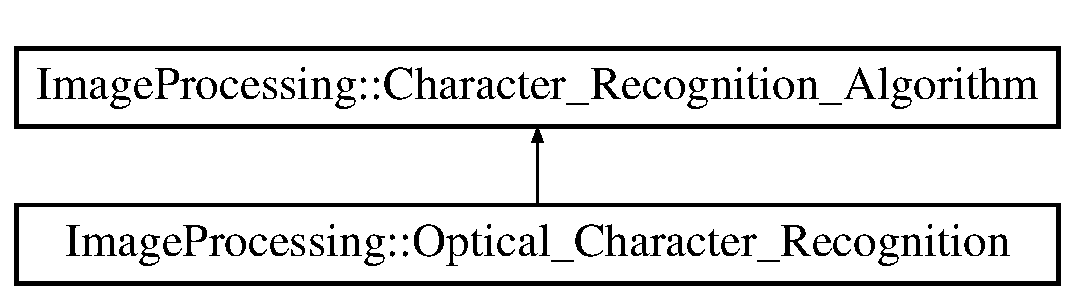
\includegraphics[height=2.000000cm]{class_image_processing_1_1_optical___character___recognition}
\end{center}
\end{figure}
\subsection*{Public Member Functions}
\begin{DoxyCompactItemize}
\item 
\mbox{\Hypertarget{class_image_processing_1_1_optical___character___recognition_a16ff8e4bcc1f780ca6d04f996f35ba94}\label{class_image_processing_1_1_optical___character___recognition_a16ff8e4bcc1f780ca6d04f996f35ba94}} 
std\+::pair$<$ int, int $>$ \mbox{\hyperlink{class_image_processing_1_1_optical___character___recognition_a16ff8e4bcc1f780ca6d04f996f35ba94}{detect\+\_\+digit}} (cv\+::\+Mat \&image)
\begin{DoxyCompactList}\small\item\em the (virtual) function that runs the recognition engine \end{DoxyCompactList}\item 
\mbox{\Hypertarget{class_image_processing_1_1_optical___character___recognition_aa64266ee48775f5f4650b0a9c2650b99}\label{class_image_processing_1_1_optical___character___recognition_aa64266ee48775f5f4650b0a9c2650b99}} 
int {\bfseries detect\+\_\+digit} (tesseract\+::\+Tess\+Base\+A\+PI $\ast$\&O\+CR, cv\+::\+Mat \&image)
\item 
\mbox{\Hypertarget{class_image_processing_1_1_optical___character___recognition_a3d771aa1f61b0b2f96bc09310c18a001}\label{class_image_processing_1_1_optical___character___recognition_a3d771aa1f61b0b2f96bc09310c18a001}} 
void {\bfseries get\+Result} (tesseract\+::\+Tess\+Base\+A\+PI $\ast$\&ocr, cv\+::\+Mat \&img, int \&result)
\end{DoxyCompactItemize}
\subsection*{Public Attributes}
\begin{DoxyCompactItemize}
\item 
\mbox{\Hypertarget{class_image_processing_1_1_optical___character___recognition_a6352d6777c7e6869de7a5840869f7e8e}\label{class_image_processing_1_1_optical___character___recognition_a6352d6777c7e6869de7a5840869f7e8e}} 
tesseract\+::\+Tess\+Base\+A\+PI $\ast$ {\bfseries ocr} = new tesseract\+::\+Tess\+Base\+A\+PI()
\end{DoxyCompactItemize}


\subsection{Detailed Description}
O\+CP algorithm from tesseract library. 

The documentation for this class was generated from the following file\+:\begin{DoxyCompactItemize}
\item 
Optical\+\_\+\+Character\+\_\+\+Recognition.\+hpp\end{DoxyCompactItemize}

\hypertarget{class_path2_d_1_1_path}{}\section{Path2D\+:\+:Path Class Reference}
\label{class_path2_d_1_1_path}\index{Path2\+D\+::\+Path@{Path2\+D\+::\+Path}}
\subsection*{Public Member Functions}
\begin{DoxyCompactItemize}
\item 
\mbox{\hyperlink{class_path2_d_1_1_path_ae91ac6b923538c7c6ba6645f5866b848}{Path}} (\mbox{\hyperlink{class_path2_d_1_1_element_1_1_position}{Position}} start\+\_\+point, \mbox{\hyperlink{class_path2_d_1_1_element_1_1_position}{Position}} end\+\_\+point, double curvature, \mbox{\hyperlink{class_map}{Map}} $\ast$map\+\_\+i)
\begin{DoxyCompactList}\small\item\em given the start point and the end point is able to find the best path \end{DoxyCompactList}\item 
\mbox{\Hypertarget{class_path2_d_1_1_path_ab8f8d4c9428e57dd03a62e7d4e1f5fad}\label{class_path2_d_1_1_path_ab8f8d4c9428e57dd03a62e7d4e1f5fad}} 
{\footnotesize template$<$class T $>$ }\\{\bfseries Path} (\mbox{\hyperlink{class_path2_d_1_1_element_1_1_position}{Position}} start\+\_\+point, \mbox{\hyperlink{class_path2_d_1_1_element_1_1_position}{Position}} end\+\_\+point, double curvature, \mbox{\hyperlink{class_map}{Map}} $\ast$map\+\_\+i, T $\ast$path\+Finder, bool complex=true)
\item 
\mbox{\Hypertarget{class_path2_d_1_1_path_a960942babbfcb89c8b153b7fe18b84a3}\label{class_path2_d_1_1_path_a960942babbfcb89c8b153b7fe18b84a3}} 
{\footnotesize template$<$class T $>$ }\\{\bfseries Path} (\mbox{\hyperlink{class_path2_d_1_1_element_1_1_path_coordinates}{Path\+Coordinates}} coordinates, \mbox{\hyperlink{class_map}{Map}} $\ast$map, T $\ast$path\+Finder, bool complex=true)
\item 
\mbox{\Hypertarget{class_path2_d_1_1_path_a4f06b4846dfb847641c0d96539e000b3}\label{class_path2_d_1_1_path_a4f06b4846dfb847641c0d96539e000b3}} 
\mbox{\hyperlink{class_path2_d_1_1_path_a4f06b4846dfb847641c0d96539e000b3}{Path}} (\mbox{\hyperlink{class_path2_d_1_1_path}{Path}} path1, \mbox{\hyperlink{class_path2_d_1_1_path}{Path}} path2)
\begin{DoxyCompactList}\small\item\em constructs a new path out of two existant path objects \end{DoxyCompactList}\item 
\mbox{\Hypertarget{class_path2_d_1_1_path_a50fcaf16012fb0bdc3054bfa2f2af09e}\label{class_path2_d_1_1_path_a50fcaf16012fb0bdc3054bfa2f2af09e}} 
void \mbox{\hyperlink{class_path2_d_1_1_path_a50fcaf16012fb0bdc3054bfa2f2af09e}{find\+Path}} ()
\begin{DoxyCompactList}\small\item\em function that detects the best path, for now uses only dubins path \end{DoxyCompactList}\item 
\mbox{\Hypertarget{class_path2_d_1_1_path_a6ded1282950f7fc212833c114720c68f}\label{class_path2_d_1_1_path_a6ded1282950f7fc212833c114720c68f}} 
void {\bfseries find\+Path\+Simple} ()
\item 
\mbox{\Hypertarget{class_path2_d_1_1_path_a695ce11815d37ed6a5aba1ee5db679e5}\label{class_path2_d_1_1_path_a695ce11815d37ed6a5aba1ee5db679e5}} 
void \mbox{\hyperlink{class_path2_d_1_1_path_a695ce11815d37ed6a5aba1ee5db679e5}{set\+Lines}} (std\+::vector$<$ \mbox{\hyperlink{class_path2_d_1_1_element_1_1_line}{Line}} $>$)
\begin{DoxyCompactList}\small\item\em set the lines of the path \end{DoxyCompactList}\item 
std\+::vector$<$ \mbox{\hyperlink{class_path2_d_1_1_element_1_1_line}{Line}} $>$ \mbox{\hyperlink{class_path2_d_1_1_path_a8961bcc1f2c03640028e181c4d7af163}{get\+Lines}} ()
\begin{DoxyCompactList}\small\item\em return a vector of lines \end{DoxyCompactList}\item 
void \mbox{\hyperlink{class_path2_d_1_1_path_a7e21bacbade3e302c5db5499cee1428f}{set\+Start\+Point}} (\mbox{\hyperlink{class_path2_d_1_1_element_1_1_position}{Position}} start\+\_\+point)
\begin{DoxyCompactList}\small\item\em set the start point of the path \end{DoxyCompactList}\item 
\mbox{\hyperlink{class_path2_d_1_1_element_1_1_position}{Position}} \mbox{\hyperlink{class_path2_d_1_1_path_acf811e8439f1e603050b74b34acd6814}{get\+Start\+Point}} ()
\begin{DoxyCompactList}\small\item\em return the start point of the path \end{DoxyCompactList}\item 
void \mbox{\hyperlink{class_path2_d_1_1_path_ae689288570f86c53e4e293ad506c9eb2}{set\+End\+Point}} (\mbox{\hyperlink{class_path2_d_1_1_element_1_1_position}{Position}} end\+\_\+point)
\begin{DoxyCompactList}\small\item\em set the end point of the path \end{DoxyCompactList}\item 
\mbox{\hyperlink{class_path2_d_1_1_element_1_1_position}{Position}} \mbox{\hyperlink{class_path2_d_1_1_path_a66b401fb426001c93d14f4a140834ee2}{get\+End\+Point}} ()
\begin{DoxyCompactList}\small\item\em return the end point of the path \end{DoxyCompactList}\item 
void \mbox{\hyperlink{class_path2_d_1_1_path_a52e9610d2c077a374bdf4d3bf7dd97e0}{set\+Max\+Curvature}} (double curvature)
\begin{DoxyCompactList}\small\item\em set max curvature of the path \end{DoxyCompactList}\item 
double \mbox{\hyperlink{class_path2_d_1_1_path_a250605196731ec8e482dcb31673a6384}{get\+Max\+Curvature}} ()
\begin{DoxyCompactList}\small\item\em return of max curvature of the path \end{DoxyCompactList}\item 
void \mbox{\hyperlink{class_path2_d_1_1_path_aa49a4a999498f68d339e049fcc176776}{set\+Length}} (double length)
\begin{DoxyCompactList}\small\item\em set the length of the path \end{DoxyCompactList}\item 
double \mbox{\hyperlink{class_path2_d_1_1_path_a5460a949ed5a26df41cd81a7884dc144}{get\+Length}} ()
\begin{DoxyCompactList}\small\item\em return the length of the path \end{DoxyCompactList}\item 
\mbox{\Hypertarget{class_path2_d_1_1_path_a21e3c84c7dc061af4ffdc03df59ff283}\label{class_path2_d_1_1_path_a21e3c84c7dc061af4ffdc03df59ff283}} 
void {\bfseries set\+Map} (\mbox{\hyperlink{class_map}{Map}} $\ast$map\+\_\+i)
\item 
\mbox{\Hypertarget{class_path2_d_1_1_path_afb07c5b028be626ffe3b6dd2e4a51959}\label{class_path2_d_1_1_path_afb07c5b028be626ffe3b6dd2e4a51959}} 
\mbox{\hyperlink{class_map}{Map}} $\ast$ {\bfseries get\+Map} ()
\item 
\mbox{\Hypertarget{class_path2_d_1_1_path_a7c07e2a15c8f7b912de69a5355174f23}\label{class_path2_d_1_1_path_a7c07e2a15c8f7b912de69a5355174f23}} 
{\footnotesize template$<$class T $>$ }\\void {\bfseries set\+Finder} (\mbox{\hyperlink{class_path2_d_1_1_element_1_1_path_coordinates}{Path\+Coordinates}} pc)
\end{DoxyCompactItemize}
\subsection*{Static Public Member Functions}
\begin{DoxyCompactItemize}
\item 
\mbox{\Hypertarget{class_path2_d_1_1_path_a7b0e3d48bc19de3e546e322d80437a52}\label{class_path2_d_1_1_path_a7b0e3d48bc19de3e546e322d80437a52}} 
{\footnotesize template$<$class T $>$ }\\static void \mbox{\hyperlink{class_path2_d_1_1_path_a7b0e3d48bc19de3e546e322d80437a52}{split}} (\mbox{\hyperlink{class_path2_d_1_1_path}{Path}} \&path, cv\+::\+Point intermediate)
\begin{DoxyCompactList}\small\item\em splits a path so it goes over an interediate point \end{DoxyCompactList}\end{DoxyCompactItemize}
\subsection*{Public Attributes}
\begin{DoxyCompactItemize}
\item 
\mbox{\Hypertarget{class_path2_d_1_1_path_ab306f2171e6829314ed3f92f75132b58}\label{class_path2_d_1_1_path_ab306f2171e6829314ed3f92f75132b58}} 
\mbox{\hyperlink{class_path2_d_1_1_element_1_1_position}{Position}} {\bfseries start\+\_\+point}
\item 
\mbox{\Hypertarget{class_path2_d_1_1_path_ab53e409ea5e8b47f1b125cec56f90552}\label{class_path2_d_1_1_path_ab53e409ea5e8b47f1b125cec56f90552}} 
\mbox{\hyperlink{class_path2_d_1_1_element_1_1_position}{Position}} {\bfseries end\+\_\+point}
\item 
\mbox{\Hypertarget{class_path2_d_1_1_path_add4022211d8ce266c0d9aa088daff289}\label{class_path2_d_1_1_path_add4022211d8ce266c0d9aa088daff289}} 
double {\bfseries max\+Curvature}
\item 
\mbox{\Hypertarget{class_path2_d_1_1_path_a654d60629e1d23f57d4ff99604ebf07a}\label{class_path2_d_1_1_path_a654d60629e1d23f57d4ff99604ebf07a}} 
std\+::vector$<$ \mbox{\hyperlink{class_path2_d_1_1_element_1_1_line}{Line}} $>$ {\bfseries lines}
\item 
\mbox{\Hypertarget{class_path2_d_1_1_path_acd25ac5dc56b47600cf7efa8ba5ae3ac}\label{class_path2_d_1_1_path_acd25ac5dc56b47600cf7efa8ba5ae3ac}} 
double {\bfseries length}
\item 
\mbox{\Hypertarget{class_path2_d_1_1_path_ae8bacd1d5855465b7e2f6f540e1e3e88}\label{class_path2_d_1_1_path_ae8bacd1d5855465b7e2f6f540e1e3e88}} 
\mbox{\hyperlink{class_map}{Map}} $\ast$ {\bfseries map}
\end{DoxyCompactItemize}


\subsection{Constructor \& Destructor Documentation}
\mbox{\Hypertarget{class_path2_d_1_1_path_ae91ac6b923538c7c6ba6645f5866b848}\label{class_path2_d_1_1_path_ae91ac6b923538c7c6ba6645f5866b848}} 
\index{Path2\+D\+::\+Path@{Path2\+D\+::\+Path}!Path@{Path}}
\index{Path@{Path}!Path2\+D\+::\+Path@{Path2\+D\+::\+Path}}
\subsubsection{\texorpdfstring{Path()}{Path()}}
{\footnotesize\ttfamily Path2\+D\+::\+Path\+::\+Path (\begin{DoxyParamCaption}\item[{\mbox{\hyperlink{class_path2_d_1_1_element_1_1_position}{Position}}}]{start\+\_\+point,  }\item[{\mbox{\hyperlink{class_path2_d_1_1_element_1_1_position}{Position}}}]{end\+\_\+point,  }\item[{double}]{curvature,  }\item[{\mbox{\hyperlink{class_map}{Map}} $\ast$}]{map\+\_\+i }\end{DoxyParamCaption})}



given the start point and the end point is able to find the best path 


\begin{DoxyParams}{Parameters}
{\em start\+\_\+point} & start point \\
\hline
{\em end\+\_\+point} & end point \\
\hline
\end{DoxyParams}


\subsection{Member Function Documentation}
\mbox{\Hypertarget{class_path2_d_1_1_path_a66b401fb426001c93d14f4a140834ee2}\label{class_path2_d_1_1_path_a66b401fb426001c93d14f4a140834ee2}} 
\index{Path2\+D\+::\+Path@{Path2\+D\+::\+Path}!get\+End\+Point@{get\+End\+Point}}
\index{get\+End\+Point@{get\+End\+Point}!Path2\+D\+::\+Path@{Path2\+D\+::\+Path}}
\subsubsection{\texorpdfstring{get\+End\+Point()}{getEndPoint()}}
{\footnotesize\ttfamily \mbox{\hyperlink{class_path2_d_1_1_element_1_1_position}{Position}} Path2\+D\+::\+Path\+::get\+End\+Point (\begin{DoxyParamCaption}{ }\end{DoxyParamCaption})}



return the end point of the path 

\begin{DoxyReturn}{Returns}
the end point of the path 
\end{DoxyReturn}
\mbox{\Hypertarget{class_path2_d_1_1_path_a5460a949ed5a26df41cd81a7884dc144}\label{class_path2_d_1_1_path_a5460a949ed5a26df41cd81a7884dc144}} 
\index{Path2\+D\+::\+Path@{Path2\+D\+::\+Path}!get\+Length@{get\+Length}}
\index{get\+Length@{get\+Length}!Path2\+D\+::\+Path@{Path2\+D\+::\+Path}}
\subsubsection{\texorpdfstring{get\+Length()}{getLength()}}
{\footnotesize\ttfamily double Path2\+D\+::\+Path\+::get\+Length (\begin{DoxyParamCaption}{ }\end{DoxyParamCaption})}



return the length of the path 

\begin{DoxyReturn}{Returns}
the length 

the length 
\end{DoxyReturn}
\mbox{\Hypertarget{class_path2_d_1_1_path_a8961bcc1f2c03640028e181c4d7af163}\label{class_path2_d_1_1_path_a8961bcc1f2c03640028e181c4d7af163}} 
\index{Path2\+D\+::\+Path@{Path2\+D\+::\+Path}!get\+Lines@{get\+Lines}}
\index{get\+Lines@{get\+Lines}!Path2\+D\+::\+Path@{Path2\+D\+::\+Path}}
\subsubsection{\texorpdfstring{get\+Lines()}{getLines()}}
{\footnotesize\ttfamily std\+::vector$<$\mbox{\hyperlink{class_path2_d_1_1_element_1_1_line}{Line}}$>$ Path2\+D\+::\+Path\+::get\+Lines (\begin{DoxyParamCaption}{ }\end{DoxyParamCaption})}



return a vector of lines 

\begin{DoxyReturn}{Returns}
vector of lines 
\end{DoxyReturn}
\mbox{\Hypertarget{class_path2_d_1_1_path_a250605196731ec8e482dcb31673a6384}\label{class_path2_d_1_1_path_a250605196731ec8e482dcb31673a6384}} 
\index{Path2\+D\+::\+Path@{Path2\+D\+::\+Path}!get\+Max\+Curvature@{get\+Max\+Curvature}}
\index{get\+Max\+Curvature@{get\+Max\+Curvature}!Path2\+D\+::\+Path@{Path2\+D\+::\+Path}}
\subsubsection{\texorpdfstring{get\+Max\+Curvature()}{getMaxCurvature()}}
{\footnotesize\ttfamily double Path2\+D\+::\+Path\+::get\+Max\+Curvature (\begin{DoxyParamCaption}{ }\end{DoxyParamCaption})}



return of max curvature of the path 

\begin{DoxyReturn}{Returns}
the max curvature of the path 
\end{DoxyReturn}
\mbox{\Hypertarget{class_path2_d_1_1_path_acf811e8439f1e603050b74b34acd6814}\label{class_path2_d_1_1_path_acf811e8439f1e603050b74b34acd6814}} 
\index{Path2\+D\+::\+Path@{Path2\+D\+::\+Path}!get\+Start\+Point@{get\+Start\+Point}}
\index{get\+Start\+Point@{get\+Start\+Point}!Path2\+D\+::\+Path@{Path2\+D\+::\+Path}}
\subsubsection{\texorpdfstring{get\+Start\+Point()}{getStartPoint()}}
{\footnotesize\ttfamily \mbox{\hyperlink{class_path2_d_1_1_element_1_1_position}{Position}} Path2\+D\+::\+Path\+::get\+Start\+Point (\begin{DoxyParamCaption}{ }\end{DoxyParamCaption})}



return the start point of the path 

\begin{DoxyReturn}{Returns}
the start point of the path 
\end{DoxyReturn}
\mbox{\Hypertarget{class_path2_d_1_1_path_ae689288570f86c53e4e293ad506c9eb2}\label{class_path2_d_1_1_path_ae689288570f86c53e4e293ad506c9eb2}} 
\index{Path2\+D\+::\+Path@{Path2\+D\+::\+Path}!set\+End\+Point@{set\+End\+Point}}
\index{set\+End\+Point@{set\+End\+Point}!Path2\+D\+::\+Path@{Path2\+D\+::\+Path}}
\subsubsection{\texorpdfstring{set\+End\+Point()}{setEndPoint()}}
{\footnotesize\ttfamily void Path2\+D\+::\+Path\+::set\+End\+Point (\begin{DoxyParamCaption}\item[{\mbox{\hyperlink{class_path2_d_1_1_element_1_1_position}{Position}}}]{end\+\_\+point }\end{DoxyParamCaption})}



set the end point of the path 


\begin{DoxyParams}{Parameters}
{\em end\+\_\+point} & the end point of the path \\
\hline
\end{DoxyParams}
\mbox{\Hypertarget{class_path2_d_1_1_path_aa49a4a999498f68d339e049fcc176776}\label{class_path2_d_1_1_path_aa49a4a999498f68d339e049fcc176776}} 
\index{Path2\+D\+::\+Path@{Path2\+D\+::\+Path}!set\+Length@{set\+Length}}
\index{set\+Length@{set\+Length}!Path2\+D\+::\+Path@{Path2\+D\+::\+Path}}
\subsubsection{\texorpdfstring{set\+Length()}{setLength()}}
{\footnotesize\ttfamily void Path2\+D\+::\+Path\+::set\+Length (\begin{DoxyParamCaption}\item[{double}]{length }\end{DoxyParamCaption})}



set the length of the path 


\begin{DoxyParams}{Parameters}
{\em length} & length of the path \\
\hline
\end{DoxyParams}
\mbox{\Hypertarget{class_path2_d_1_1_path_a52e9610d2c077a374bdf4d3bf7dd97e0}\label{class_path2_d_1_1_path_a52e9610d2c077a374bdf4d3bf7dd97e0}} 
\index{Path2\+D\+::\+Path@{Path2\+D\+::\+Path}!set\+Max\+Curvature@{set\+Max\+Curvature}}
\index{set\+Max\+Curvature@{set\+Max\+Curvature}!Path2\+D\+::\+Path@{Path2\+D\+::\+Path}}
\subsubsection{\texorpdfstring{set\+Max\+Curvature()}{setMaxCurvature()}}
{\footnotesize\ttfamily void Path2\+D\+::\+Path\+::set\+Max\+Curvature (\begin{DoxyParamCaption}\item[{double}]{curvature }\end{DoxyParamCaption})}



set max curvature of the path 


\begin{DoxyParams}{Parameters}
{\em curvature} & max curvature of the path \\
\hline
\end{DoxyParams}
\mbox{\Hypertarget{class_path2_d_1_1_path_a7e21bacbade3e302c5db5499cee1428f}\label{class_path2_d_1_1_path_a7e21bacbade3e302c5db5499cee1428f}} 
\index{Path2\+D\+::\+Path@{Path2\+D\+::\+Path}!set\+Start\+Point@{set\+Start\+Point}}
\index{set\+Start\+Point@{set\+Start\+Point}!Path2\+D\+::\+Path@{Path2\+D\+::\+Path}}
\subsubsection{\texorpdfstring{set\+Start\+Point()}{setStartPoint()}}
{\footnotesize\ttfamily void Path2\+D\+::\+Path\+::set\+Start\+Point (\begin{DoxyParamCaption}\item[{\mbox{\hyperlink{class_path2_d_1_1_element_1_1_position}{Position}}}]{start\+\_\+point }\end{DoxyParamCaption})}



set the start point of the path 


\begin{DoxyParams}{Parameters}
{\em start\+\_\+point} & start point of the path \\
\hline
\end{DoxyParams}


The documentation for this class was generated from the following file\+:\begin{DoxyCompactItemize}
\item 
Path.\+hpp\end{DoxyCompactItemize}

\hypertarget{class_path2_d_1_1_element_1_1_path_coordinates}{}\section{Path2D\+:\+:Element\+:\+:Path\+Coordinates Class Reference}
\label{class_path2_d_1_1_element_1_1_path_coordinates}\index{Path2\+D\+::\+Element\+::\+Path\+Coordinates@{Path2\+D\+::\+Element\+::\+Path\+Coordinates}}


class for storing data that describes the path  




{\ttfamily \#include $<$Path\+Coordinates.\+hpp$>$}

\subsection*{Public Member Functions}
\begin{DoxyCompactItemize}
\item 
\mbox{\hyperlink{class_path2_d_1_1_element_1_1_path_coordinates_a63f9e5d25a023ed5aa42d440ef095afa}{Path\+Coordinates}} (\mbox{\hyperlink{class_path2_d_1_1_element_1_1_position}{Position}} position\+\_\+in, \mbox{\hyperlink{class_path2_d_1_1_element_1_1_position}{Position}} position\+\_\+fin, double curvature\+\_\+p)
\begin{DoxyCompactList}\small\item\em constructor of the \mbox{\hyperlink{class_path2_d_1_1_element_1_1_path_coordinates}{Path\+Coordinates}} class \end{DoxyCompactList}\item 
\mbox{\Hypertarget{class_path2_d_1_1_element_1_1_path_coordinates_a67ac69efd20e7567548bf95df80095ab}\label{class_path2_d_1_1_element_1_1_path_coordinates_a67ac69efd20e7567548bf95df80095ab}} 
\mbox{\hyperlink{class_path2_d_1_1_element_1_1_path_coordinates_a67ac69efd20e7567548bf95df80095ab}{$\sim$\+Path\+Coordinates}} ()
\begin{DoxyCompactList}\small\item\em destructor of the \mbox{\hyperlink{class_path2_d_1_1_element_1_1_path_coordinates}{Path\+Coordinates}} class \end{DoxyCompactList}\item 
void \mbox{\hyperlink{class_path2_d_1_1_element_1_1_path_coordinates_aa186070d9a737ae97904fdadfb72aad7}{set\+Positions}} (\mbox{\hyperlink{class_path2_d_1_1_element_1_1_position}{Position}} position\+\_\+in, \mbox{\hyperlink{class_path2_d_1_1_element_1_1_position}{Position}} position\+\_\+fin)
\item 
\mbox{\hyperlink{class_path2_d_1_1_element_1_1_position}{Position}} \mbox{\hyperlink{class_path2_d_1_1_element_1_1_path_coordinates_aed77d05b5c06d46d95f92a2869006e13}{get\+Initial\+Position}} ()
\begin{DoxyCompactList}\small\item\em return the initial position of the path \end{DoxyCompactList}\item 
\mbox{\hyperlink{class_path2_d_1_1_element_1_1_position}{Position}} \mbox{\hyperlink{class_path2_d_1_1_element_1_1_path_coordinates_a169ed599c2de6960c5fe74ea559ea798}{get\+Final\+Position}} ()
\begin{DoxyCompactList}\small\item\em return the final position of the path \end{DoxyCompactList}\item 
double \mbox{\hyperlink{class_path2_d_1_1_element_1_1_path_coordinates_a0af78108850ec2152b187cb18f48cb2b}{get\+Max\+Curvature}} ()
\begin{DoxyCompactList}\small\item\em return the curvature of the path \end{DoxyCompactList}\item 
void \mbox{\hyperlink{class_path2_d_1_1_element_1_1_path_coordinates_a35528f5a799aadeaf6b1c5b04459af5b}{set\+Max\+Curvature}} (double curvature\+\_\+p)
\begin{DoxyCompactList}\small\item\em set the max curvature of the path \end{DoxyCompactList}\end{DoxyCompactItemize}


\subsection{Detailed Description}
class for storing data that describes the path 

\subsection{Constructor \& Destructor Documentation}
\mbox{\Hypertarget{class_path2_d_1_1_element_1_1_path_coordinates_a63f9e5d25a023ed5aa42d440ef095afa}\label{class_path2_d_1_1_element_1_1_path_coordinates_a63f9e5d25a023ed5aa42d440ef095afa}} 
\index{Path2\+D\+::\+Element\+::\+Path\+Coordinates@{Path2\+D\+::\+Element\+::\+Path\+Coordinates}!Path\+Coordinates@{Path\+Coordinates}}
\index{Path\+Coordinates@{Path\+Coordinates}!Path2\+D\+::\+Element\+::\+Path\+Coordinates@{Path2\+D\+::\+Element\+::\+Path\+Coordinates}}
\subsubsection{\texorpdfstring{Path\+Coordinates()}{PathCoordinates()}}
{\footnotesize\ttfamily Path2\+D\+::\+Element\+::\+Path\+Coordinates\+::\+Path\+Coordinates (\begin{DoxyParamCaption}\item[{\mbox{\hyperlink{class_path2_d_1_1_element_1_1_position}{Position}}}]{position\+\_\+in,  }\item[{\mbox{\hyperlink{class_path2_d_1_1_element_1_1_position}{Position}}}]{position\+\_\+fin,  }\item[{double}]{curvature\+\_\+p }\end{DoxyParamCaption})}



constructor of the \mbox{\hyperlink{class_path2_d_1_1_element_1_1_path_coordinates}{Path\+Coordinates}} class 


\begin{DoxyParams}{Parameters}
{\em position\+\_\+in} & initial position of the path \\
\hline
{\em position\+\_\+fin} & final position if the path \\
\hline
{\em curvature\+\_\+p} & curvature of the path \\
\hline
\end{DoxyParams}


\subsection{Member Function Documentation}
\mbox{\Hypertarget{class_path2_d_1_1_element_1_1_path_coordinates_a169ed599c2de6960c5fe74ea559ea798}\label{class_path2_d_1_1_element_1_1_path_coordinates_a169ed599c2de6960c5fe74ea559ea798}} 
\index{Path2\+D\+::\+Element\+::\+Path\+Coordinates@{Path2\+D\+::\+Element\+::\+Path\+Coordinates}!get\+Final\+Position@{get\+Final\+Position}}
\index{get\+Final\+Position@{get\+Final\+Position}!Path2\+D\+::\+Element\+::\+Path\+Coordinates@{Path2\+D\+::\+Element\+::\+Path\+Coordinates}}
\subsubsection{\texorpdfstring{get\+Final\+Position()}{getFinalPosition()}}
{\footnotesize\ttfamily \mbox{\hyperlink{class_path2_d_1_1_element_1_1_position}{Position}} Path2\+D\+::\+Element\+::\+Path\+Coordinates\+::get\+Final\+Position (\begin{DoxyParamCaption}{ }\end{DoxyParamCaption})}



return the final position of the path 

\begin{DoxyReturn}{Returns}
the final position of the path 
\end{DoxyReturn}
\mbox{\Hypertarget{class_path2_d_1_1_element_1_1_path_coordinates_aed77d05b5c06d46d95f92a2869006e13}\label{class_path2_d_1_1_element_1_1_path_coordinates_aed77d05b5c06d46d95f92a2869006e13}} 
\index{Path2\+D\+::\+Element\+::\+Path\+Coordinates@{Path2\+D\+::\+Element\+::\+Path\+Coordinates}!get\+Initial\+Position@{get\+Initial\+Position}}
\index{get\+Initial\+Position@{get\+Initial\+Position}!Path2\+D\+::\+Element\+::\+Path\+Coordinates@{Path2\+D\+::\+Element\+::\+Path\+Coordinates}}
\subsubsection{\texorpdfstring{get\+Initial\+Position()}{getInitialPosition()}}
{\footnotesize\ttfamily \mbox{\hyperlink{class_path2_d_1_1_element_1_1_position}{Position}} Path2\+D\+::\+Element\+::\+Path\+Coordinates\+::get\+Initial\+Position (\begin{DoxyParamCaption}{ }\end{DoxyParamCaption})}



return the initial position of the path 

\begin{DoxyReturn}{Returns}
the initial position of the path 
\end{DoxyReturn}
\mbox{\Hypertarget{class_path2_d_1_1_element_1_1_path_coordinates_a0af78108850ec2152b187cb18f48cb2b}\label{class_path2_d_1_1_element_1_1_path_coordinates_a0af78108850ec2152b187cb18f48cb2b}} 
\index{Path2\+D\+::\+Element\+::\+Path\+Coordinates@{Path2\+D\+::\+Element\+::\+Path\+Coordinates}!get\+Max\+Curvature@{get\+Max\+Curvature}}
\index{get\+Max\+Curvature@{get\+Max\+Curvature}!Path2\+D\+::\+Element\+::\+Path\+Coordinates@{Path2\+D\+::\+Element\+::\+Path\+Coordinates}}
\subsubsection{\texorpdfstring{get\+Max\+Curvature()}{getMaxCurvature()}}
{\footnotesize\ttfamily double Path2\+D\+::\+Element\+::\+Path\+Coordinates\+::get\+Max\+Curvature (\begin{DoxyParamCaption}{ }\end{DoxyParamCaption})}



return the curvature of the path 

\begin{DoxyReturn}{Returns}
the curvature of the path 
\end{DoxyReturn}
\mbox{\Hypertarget{class_path2_d_1_1_element_1_1_path_coordinates_a35528f5a799aadeaf6b1c5b04459af5b}\label{class_path2_d_1_1_element_1_1_path_coordinates_a35528f5a799aadeaf6b1c5b04459af5b}} 
\index{Path2\+D\+::\+Element\+::\+Path\+Coordinates@{Path2\+D\+::\+Element\+::\+Path\+Coordinates}!set\+Max\+Curvature@{set\+Max\+Curvature}}
\index{set\+Max\+Curvature@{set\+Max\+Curvature}!Path2\+D\+::\+Element\+::\+Path\+Coordinates@{Path2\+D\+::\+Element\+::\+Path\+Coordinates}}
\subsubsection{\texorpdfstring{set\+Max\+Curvature()}{setMaxCurvature()}}
{\footnotesize\ttfamily void Path2\+D\+::\+Element\+::\+Path\+Coordinates\+::set\+Max\+Curvature (\begin{DoxyParamCaption}\item[{double}]{curvature\+\_\+p }\end{DoxyParamCaption})}



set the max curvature of the path 


\begin{DoxyParams}{Parameters}
{\em curvature\+\_\+p} & the max curvature of the path \\
\hline
\end{DoxyParams}
\mbox{\Hypertarget{class_path2_d_1_1_element_1_1_path_coordinates_aa186070d9a737ae97904fdadfb72aad7}\label{class_path2_d_1_1_element_1_1_path_coordinates_aa186070d9a737ae97904fdadfb72aad7}} 
\index{Path2\+D\+::\+Element\+::\+Path\+Coordinates@{Path2\+D\+::\+Element\+::\+Path\+Coordinates}!set\+Positions@{set\+Positions}}
\index{set\+Positions@{set\+Positions}!Path2\+D\+::\+Element\+::\+Path\+Coordinates@{Path2\+D\+::\+Element\+::\+Path\+Coordinates}}
\subsubsection{\texorpdfstring{set\+Positions()}{setPositions()}}
{\footnotesize\ttfamily void Path2\+D\+::\+Element\+::\+Path\+Coordinates\+::set\+Positions (\begin{DoxyParamCaption}\item[{\mbox{\hyperlink{class_path2_d_1_1_element_1_1_position}{Position}}}]{position\+\_\+in,  }\item[{\mbox{\hyperlink{class_path2_d_1_1_element_1_1_position}{Position}}}]{position\+\_\+fin }\end{DoxyParamCaption})}

set the initial and the final position of the path 
\begin{DoxyParams}{Parameters}
{\em position\+\_\+in} & initial position of the path \\
\hline
{\em position\+\_\+fin} & final position of the path \\
\hline
\end{DoxyParams}


The documentation for this class was generated from the following file\+:\begin{DoxyCompactItemize}
\item 
Path\+Coordinates.\+hpp\end{DoxyCompactItemize}

\hypertarget{class_path2_d_1_1_path_finder}{}\section{Path2D\+:\+:Path\+Finder Class Reference}
\label{class_path2_d_1_1_path_finder}\index{Path2\+D\+::\+Path\+Finder@{Path2\+D\+::\+Path\+Finder}}


abstract class for finding a path between two Positions  This class is a basis for more defined classes based on this class structure. For example a Dubins\+Path\+Finder class could be used to find a path using Dubin\+Curves, or an Spline\+Path\+Finder could be made to find a Spline\+Curve. Anyway this class does not just contain the basic structure of future specialized implementations but also usefull tools every Path\+Finding algorithm needs, such as a collision detection class nested inside. Given a map object this class can be used to see if the picked path is colliding with obstacles in the map.  




{\ttfamily \#include $<$Path\+Finder.\+hpp$>$}

Inheritance diagram for Path2D\+:\+:Path\+Finder\+:\begin{figure}[H]
\begin{center}
\leavevmode
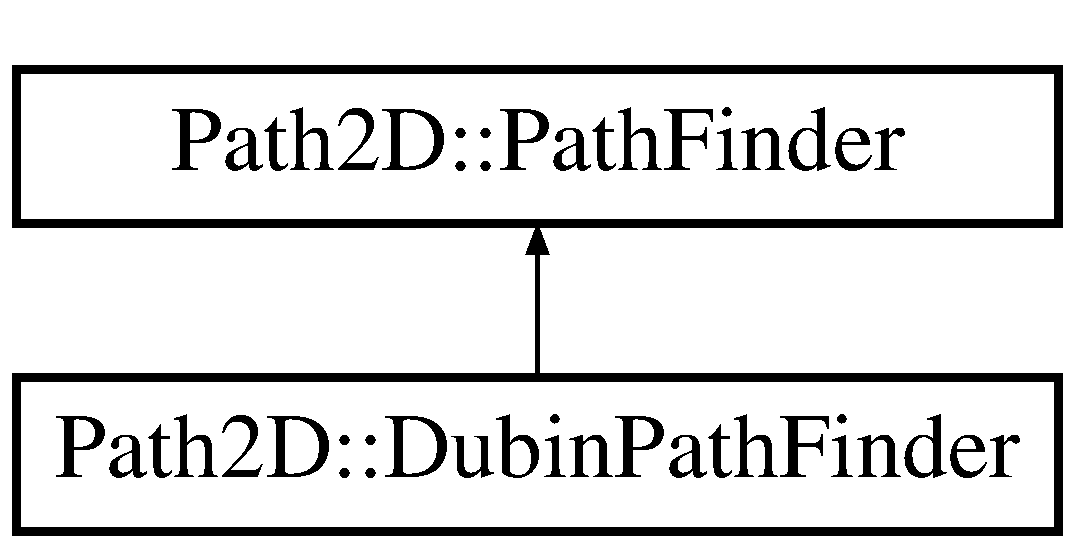
\includegraphics[height=2.000000cm]{class_path2_d_1_1_path_finder}
\end{center}
\end{figure}
\subsection*{Classes}
\begin{DoxyCompactItemize}
\item 
class \mbox{\hyperlink{class_path2_d_1_1_path_finder_1_1_collision_detector}{Collision\+Detector}}
\begin{DoxyCompactList}\small\item\em detector of collision between obstacles and path \end{DoxyCompactList}\end{DoxyCompactItemize}
\subsection*{Public Member Functions}
\begin{DoxyCompactItemize}
\item 
\mbox{\hyperlink{class_path2_d_1_1_path_finder_a0aa8bbd238985f5baa456287671551ea}{Path\+Finder}} (\mbox{\hyperlink{class_path2_d_1_1_element_1_1_path_coordinates}{Path\+Coordinates}} path\+\_\+coordinates\+\_\+i, \mbox{\hyperlink{class_map}{Map}} $\ast$map\+\_\+i)
\begin{DoxyCompactList}\small\item\em constructor of the \mbox{\hyperlink{class_path2_d_1_1_path_finder}{Path\+Finder}} class \end{DoxyCompactList}\item 
\mbox{\Hypertarget{class_path2_d_1_1_path_finder_a32bdcb63296c44e8777d0f247f2072ea}\label{class_path2_d_1_1_path_finder_a32bdcb63296c44e8777d0f247f2072ea}} 
{\bfseries Path\+Finder} (\mbox{\hyperlink{class_path2_d_1_1_element_1_1_position}{Position}} start\+\_\+point, \mbox{\hyperlink{class_path2_d_1_1_element_1_1_position}{Position}} end\+\_\+point, double curvature, \mbox{\hyperlink{class_map}{Map}} $\ast$map\+\_\+i)
\item 
\mbox{\Hypertarget{class_path2_d_1_1_path_finder_a96141cb3260846bab64d45f3a8f40515}\label{class_path2_d_1_1_path_finder_a96141cb3260846bab64d45f3a8f40515}} 
\mbox{\hyperlink{class_path2_d_1_1_path_finder_a96141cb3260846bab64d45f3a8f40515}{Path\+Finder}} ()
\begin{DoxyCompactList}\small\item\em destructor of the \mbox{\hyperlink{class_path2_d_1_1_path_finder}{Path\+Finder}} class \end{DoxyCompactList}\item 
virtual std\+::vector$<$ \mbox{\hyperlink{class_path2_d_1_1_element_1_1_line}{Line}} $>$ \mbox{\hyperlink{class_path2_d_1_1_path_finder_a5d050326067c313925d87ac37612a181}{shortest\+Path}} (std\+::vector$<$ cv\+::\+Point $>$ \&alternative\+\_\+\+Points)=0
\begin{DoxyCompactList}\small\item\em function that find the dubins shortest path and return a vector of line \end{DoxyCompactList}\end{DoxyCompactItemize}
\subsection*{Public Attributes}
\begin{DoxyCompactItemize}
\item 
\mbox{\Hypertarget{class_path2_d_1_1_path_finder_a91d4111a80bb3d5cde042169fab4337e}\label{class_path2_d_1_1_path_finder_a91d4111a80bb3d5cde042169fab4337e}} 
\mbox{\hyperlink{class_path2_d_1_1_element_1_1_path_coordinates}{Path\+Coordinates}} {\bfseries path\+\_\+coordinates} = \mbox{\hyperlink{class_path2_d_1_1_element_1_1_path_coordinates}{Path\+Coordinates}}(\mbox{\hyperlink{class_path2_d_1_1_element_1_1_position}{Position}}(), \mbox{\hyperlink{class_path2_d_1_1_element_1_1_position}{Position}}(), 0)
\item 
\mbox{\Hypertarget{class_path2_d_1_1_path_finder_a71fb23328f7dd376cce578b34441c10a}\label{class_path2_d_1_1_path_finder_a71fb23328f7dd376cce578b34441c10a}} 
double {\bfseries length}
\item 
\mbox{\Hypertarget{class_path2_d_1_1_path_finder_a9db26e8edde93af781907314b0cf2e9b}\label{class_path2_d_1_1_path_finder_a9db26e8edde93af781907314b0cf2e9b}} 
\mbox{\hyperlink{class_map}{Map}} $\ast$ {\bfseries map}
\item 
\mbox{\Hypertarget{class_path2_d_1_1_path_finder_a81fab59437d1f65f6c1a6aaf796c40ed}\label{class_path2_d_1_1_path_finder_a81fab59437d1f65f6c1a6aaf796c40ed}} 
\mbox{\hyperlink{class_path2_d_1_1_path_finder_1_1_collision_detector}{Collision\+Detector}} {\bfseries collision\+Detector}
\end{DoxyCompactItemize}


\subsection{Detailed Description}
abstract class for finding a path between two Positions  This class is a basis for more defined classes based on this class structure. For example a Dubins\+Path\+Finder class could be used to find a path using Dubin\+Curves, or an Spline\+Path\+Finder could be made to find a Spline\+Curve. Anyway this class does not just contain the basic structure of future specialized implementations but also usefull tools every Path\+Finding algorithm needs, such as a collision detection class nested inside. Given a map object this class can be used to see if the picked path is colliding with obstacles in the map. 

\subsection{Constructor \& Destructor Documentation}
\mbox{\Hypertarget{class_path2_d_1_1_path_finder_a0aa8bbd238985f5baa456287671551ea}\label{class_path2_d_1_1_path_finder_a0aa8bbd238985f5baa456287671551ea}} 
\index{Path2\+D\+::\+Path\+Finder@{Path2\+D\+::\+Path\+Finder}!Path\+Finder@{Path\+Finder}}
\index{Path\+Finder@{Path\+Finder}!Path2\+D\+::\+Path\+Finder@{Path2\+D\+::\+Path\+Finder}}
\subsubsection{\texorpdfstring{Path\+Finder()}{PathFinder()}}
{\footnotesize\ttfamily Path2\+D\+::\+Path\+Finder\+::\+Path\+Finder (\begin{DoxyParamCaption}\item[{\mbox{\hyperlink{class_path2_d_1_1_element_1_1_path_coordinates}{Path\+Coordinates}}}]{path\+\_\+coordinates\+\_\+i,  }\item[{\mbox{\hyperlink{class_map}{Map}} $\ast$}]{map\+\_\+i }\end{DoxyParamCaption})}



constructor of the \mbox{\hyperlink{class_path2_d_1_1_path_finder}{Path\+Finder}} class 


\begin{DoxyParams}{Parameters}
{\em path\+\_\+coordinates\+\_\+i} & coordinates of the path that we want to find \\
\hline
\end{DoxyParams}


\subsection{Member Function Documentation}
\mbox{\Hypertarget{class_path2_d_1_1_path_finder_a5d050326067c313925d87ac37612a181}\label{class_path2_d_1_1_path_finder_a5d050326067c313925d87ac37612a181}} 
\index{Path2\+D\+::\+Path\+Finder@{Path2\+D\+::\+Path\+Finder}!shortest\+Path@{shortest\+Path}}
\index{shortest\+Path@{shortest\+Path}!Path2\+D\+::\+Path\+Finder@{Path2\+D\+::\+Path\+Finder}}
\subsubsection{\texorpdfstring{shortest\+Path()}{shortestPath()}}
{\footnotesize\ttfamily virtual std\+::vector$<$\mbox{\hyperlink{class_path2_d_1_1_element_1_1_line}{Line}}$>$ Path2\+D\+::\+Path\+Finder\+::shortest\+Path (\begin{DoxyParamCaption}\item[{std\+::vector$<$ cv\+::\+Point $>$ \&}]{alternative\+\_\+\+Points }\end{DoxyParamCaption})\hspace{0.3cm}{\ttfamily [pure virtual]}}



function that find the dubins shortest path and return a vector of line 

\begin{DoxyItemize}
\item alternative\+\_\+\+Points a point set for every obsticle that was found along the way \begin{DoxyReturn}{Returns}
vector of lines which describes the path 
\end{DoxyReturn}
\end{DoxyItemize}


Implemented in \mbox{\hyperlink{class_path2_d_1_1_dubin_path_finder_a53d6ee86e364b403274f403af6e5088e}{Path2\+D\+::\+Dubin\+Path\+Finder}}.



The documentation for this class was generated from the following file\+:\begin{DoxyCompactItemize}
\item 
Path\+Finder.\+hpp\end{DoxyCompactItemize}

\hypertarget{class_geometry2_d_1_1_pentagon}{}\section{Geometry2D\+:\+:Pentagon Class Reference}
\label{class_geometry2_d_1_1_pentagon}\index{Geometry2\+D\+::\+Pentagon@{Geometry2\+D\+::\+Pentagon}}


Class for hadling pentagon obstacles in the map.  




{\ttfamily \#include $<$Pentagon.\+hpp$>$}

Inheritance diagram for Geometry2D\+:\+:Pentagon\+:\begin{figure}[H]
\begin{center}
\leavevmode
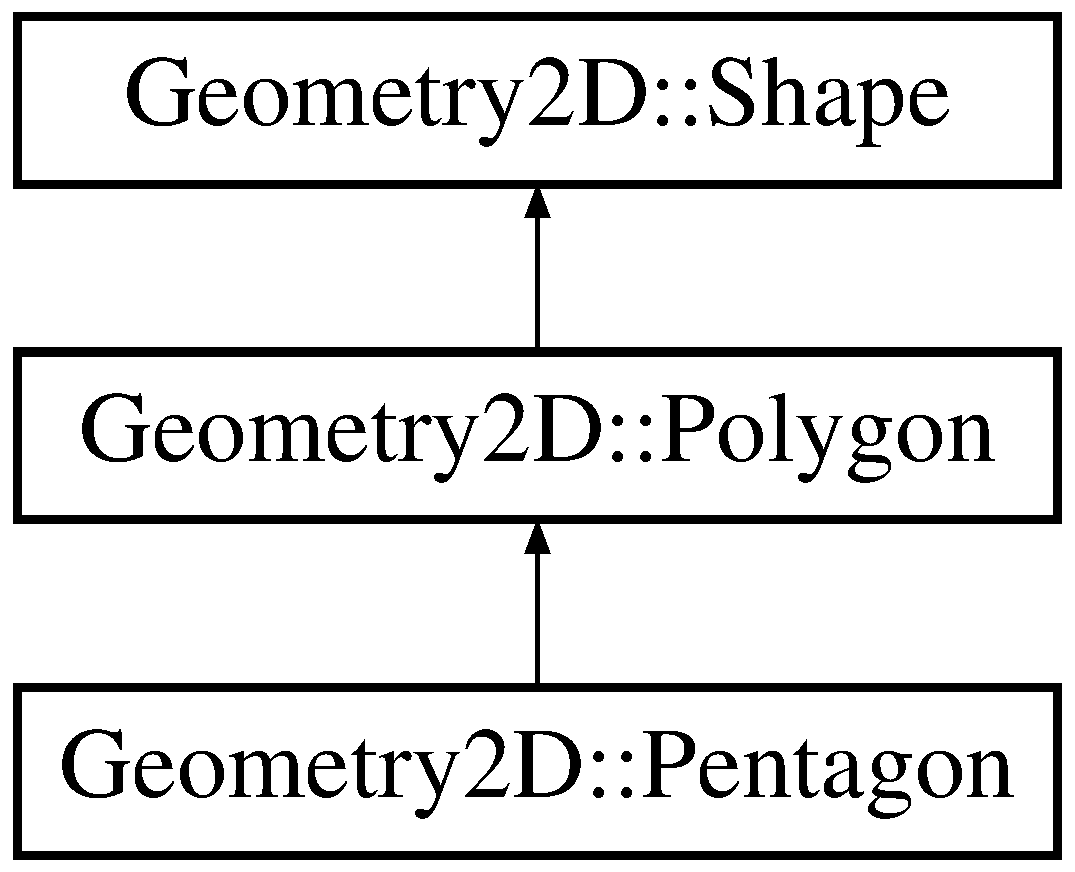
\includegraphics[height=3.000000cm]{class_geometry2_d_1_1_pentagon}
\end{center}
\end{figure}
\subsection*{Public Member Functions}
\begin{DoxyCompactItemize}
\item 
\mbox{\hyperlink{class_geometry2_d_1_1_pentagon_ab7db58850051b5fc59c5f16428020e6b}{Pentagon}} ()
\item 
\mbox{\Hypertarget{class_geometry2_d_1_1_pentagon_a0c1a7da132f79d4959988dda7a9d3ab9}\label{class_geometry2_d_1_1_pentagon_a0c1a7da132f79d4959988dda7a9d3ab9}} 
{\bfseries Pentagon} (std\+::vector$<$ cv\+::\+Point $>$ \mbox{\hyperlink{class_geometry2_d_1_1_polygon_ab965e028324c2199022da00ff7eef14b}{points}})
\item 
\mbox{\hyperlink{class_geometry2_d_1_1_pentagon_ac7b31f244f4419cc5b564a6b35d0f1fc}{$\sim$\+Pentagon}} ()
\item 
std\+::vector$<$ cv\+::\+Point $>$ \mbox{\hyperlink{class_geometry2_d_1_1_pentagon_a132f80b78a2bf41e393becaaae5b535e}{get\+Corners}} ()
\item 
void \mbox{\hyperlink{class_geometry2_d_1_1_pentagon_ae65ba44439b3fccd94c35b74b877e05f}{set\+Corners}} (std\+::vector$<$ cv\+::\+Point $>$ corners)
\item 
\mbox{\Hypertarget{class_geometry2_d_1_1_pentagon_a18a04ba60e0713eb90de37651adc9d4f}\label{class_geometry2_d_1_1_pentagon_a18a04ba60e0713eb90de37651adc9d4f}} 
void \mbox{\hyperlink{class_geometry2_d_1_1_pentagon_a18a04ba60e0713eb90de37651adc9d4f}{assign\+\_\+points}} ()
\begin{DoxyCompactList}\small\item\em assignes points to 1., 2., 3 etc point. \end{DoxyCompactList}\end{DoxyCompactItemize}
\subsection*{Additional Inherited Members}


\subsection{Detailed Description}
Class for hadling pentagon obstacles in the map. 

\subsection{Constructor \& Destructor Documentation}
\mbox{\Hypertarget{class_geometry2_d_1_1_pentagon_ab7db58850051b5fc59c5f16428020e6b}\label{class_geometry2_d_1_1_pentagon_ab7db58850051b5fc59c5f16428020e6b}} 
\index{Geometry2\+D\+::\+Pentagon@{Geometry2\+D\+::\+Pentagon}!Pentagon@{Pentagon}}
\index{Pentagon@{Pentagon}!Geometry2\+D\+::\+Pentagon@{Geometry2\+D\+::\+Pentagon}}
\subsubsection{\texorpdfstring{Pentagon()}{Pentagon()}}
{\footnotesize\ttfamily Geometry2\+D\+::\+Pentagon\+::\+Pentagon (\begin{DoxyParamCaption}{ }\end{DoxyParamCaption})}

constructor of \mbox{\hyperlink{class_geometry2_d_1_1_pentagon}{Pentagon}} class \mbox{\Hypertarget{class_geometry2_d_1_1_pentagon_ac7b31f244f4419cc5b564a6b35d0f1fc}\label{class_geometry2_d_1_1_pentagon_ac7b31f244f4419cc5b564a6b35d0f1fc}} 
\index{Geometry2\+D\+::\+Pentagon@{Geometry2\+D\+::\+Pentagon}!````~Pentagon@{$\sim$\+Pentagon}}
\index{````~Pentagon@{$\sim$\+Pentagon}!Geometry2\+D\+::\+Pentagon@{Geometry2\+D\+::\+Pentagon}}
\subsubsection{\texorpdfstring{$\sim$\+Pentagon()}{~Pentagon()}}
{\footnotesize\ttfamily Geometry2\+D\+::\+Pentagon\+::$\sim$\+Pentagon (\begin{DoxyParamCaption}{ }\end{DoxyParamCaption})}

destructor of \mbox{\hyperlink{class_geometry2_d_1_1_pentagon}{Pentagon}} class 

\subsection{Member Function Documentation}
\mbox{\Hypertarget{class_geometry2_d_1_1_pentagon_a132f80b78a2bf41e393becaaae5b535e}\label{class_geometry2_d_1_1_pentagon_a132f80b78a2bf41e393becaaae5b535e}} 
\index{Geometry2\+D\+::\+Pentagon@{Geometry2\+D\+::\+Pentagon}!get\+Corners@{get\+Corners}}
\index{get\+Corners@{get\+Corners}!Geometry2\+D\+::\+Pentagon@{Geometry2\+D\+::\+Pentagon}}
\subsubsection{\texorpdfstring{get\+Corners()}{getCorners()}}
{\footnotesize\ttfamily std\+::vector$<$cv\+::\+Point$>$ Geometry2\+D\+::\+Pentagon\+::get\+Corners (\begin{DoxyParamCaption}{ }\end{DoxyParamCaption})}

return the list of corners of the pentagons \begin{DoxyReturn}{Returns}
the list of corners of the amaz 
\end{DoxyReturn}
\mbox{\Hypertarget{class_geometry2_d_1_1_pentagon_ae65ba44439b3fccd94c35b74b877e05f}\label{class_geometry2_d_1_1_pentagon_ae65ba44439b3fccd94c35b74b877e05f}} 
\index{Geometry2\+D\+::\+Pentagon@{Geometry2\+D\+::\+Pentagon}!set\+Corners@{set\+Corners}}
\index{set\+Corners@{set\+Corners}!Geometry2\+D\+::\+Pentagon@{Geometry2\+D\+::\+Pentagon}}
\subsubsection{\texorpdfstring{set\+Corners()}{setCorners()}}
{\footnotesize\ttfamily void Geometry2\+D\+::\+Pentagon\+::set\+Corners (\begin{DoxyParamCaption}\item[{std\+::vector$<$ cv\+::\+Point $>$}]{corners }\end{DoxyParamCaption})}

set the corners of the pentagon 
\begin{DoxyParams}{Parameters}
{\em corners} & list of corners to be setted \\
\hline
\end{DoxyParams}


The documentation for this class was generated from the following file\+:\begin{DoxyCompactItemize}
\item 
Pentagon.\+hpp\end{DoxyCompactItemize}

\hypertarget{class_people}{}\section{People Class Reference}
\label{class_people}\index{People@{People}}


class for representing people in the map that have to be collected  




{\ttfamily \#include $<$People.\+hpp$>$}

Inheritance diagram for People\+:\begin{figure}[H]
\begin{center}
\leavevmode
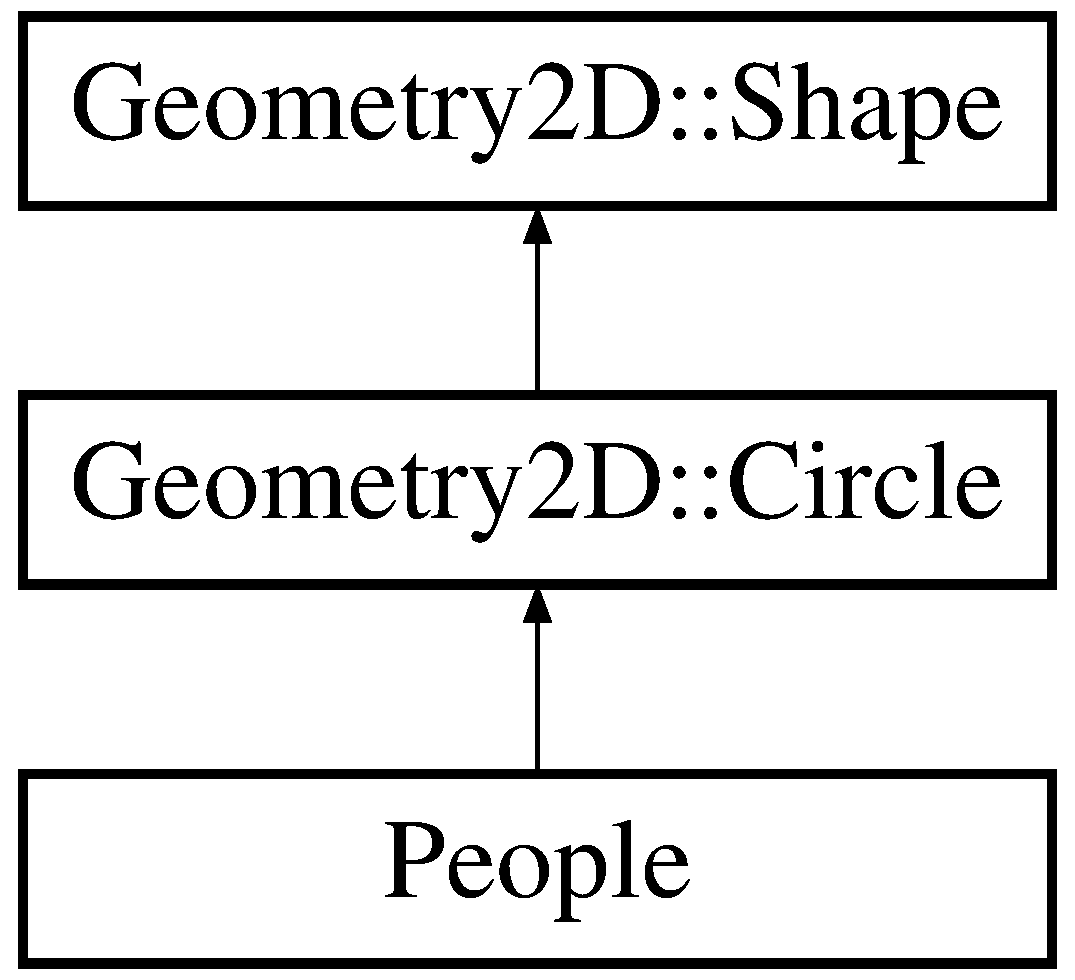
\includegraphics[height=3.000000cm]{class_people}
\end{center}
\end{figure}
\subsection*{Public Member Functions}
\begin{DoxyCompactItemize}
\item 
\mbox{\hyperlink{class_people_aae1408eddfd15a5007003ecdf1507941}{People}} ()
\item 
\mbox{\Hypertarget{class_people_abfabd2f2e27a7aa269d404e8f27f903e}\label{class_people_abfabd2f2e27a7aa269d404e8f27f903e}} 
{\bfseries People} (std\+::pair$<$ int, int $>$ digit, cv\+::\+Rect rect)
\item 
\mbox{\hyperlink{class_people_adae124857f64dadff4e1801410b3dab2}{$\sim$\+People}} ()
\end{DoxyCompactItemize}
\subsection*{Public Attributes}
\begin{DoxyCompactItemize}
\item 
\mbox{\Hypertarget{class_people_a06e995c8c3b9808db931bedb44d782c8}\label{class_people_a06e995c8c3b9808db931bedb44d782c8}} 
int \mbox{\hyperlink{class_people_a06e995c8c3b9808db931bedb44d782c8}{name}}
\begin{DoxyCompactList}\small\item\em \mbox{\hyperlink{class_people}{People}} have names -\/ represented by a digit. \end{DoxyCompactList}\item 
\mbox{\Hypertarget{class_people_a44d79c52132068763c91e308e9685e06}\label{class_people_a44d79c52132068763c91e308e9685e06}} 
int \mbox{\hyperlink{class_people_a44d79c52132068763c91e308e9685e06}{confidence}}
\begin{DoxyCompactList}\small\item\em confidence that name is the correct digit \end{DoxyCompactList}\end{DoxyCompactItemize}


\subsection{Detailed Description}
class for representing people in the map that have to be collected 

\mbox{\hyperlink{class_people}{People}} are round objects with green background that need to be collected before exiting the map. \mbox{\hyperlink{class_people}{People}} have a unique identifier given by a digit. This identifier is their name. \mbox{\hyperlink{class_people}{People}} inherit all shape characteristics of Circles, because their have circular shapes. In addition to their name and form people have a confidence level assigned to them indicating how confident the character recognition algorithm was when detecting their name. 

\subsection{Constructor \& Destructor Documentation}
\mbox{\Hypertarget{class_people_aae1408eddfd15a5007003ecdf1507941}\label{class_people_aae1408eddfd15a5007003ecdf1507941}} 
\index{People@{People}!People@{People}}
\index{People@{People}!People@{People}}
\subsubsection{\texorpdfstring{People()}{People()}}
{\footnotesize\ttfamily People\+::\+People (\begin{DoxyParamCaption}{ }\end{DoxyParamCaption})}

constructor of people class \mbox{\Hypertarget{class_people_adae124857f64dadff4e1801410b3dab2}\label{class_people_adae124857f64dadff4e1801410b3dab2}} 
\index{People@{People}!````~People@{$\sim$\+People}}
\index{````~People@{$\sim$\+People}!People@{People}}
\subsubsection{\texorpdfstring{$\sim$\+People()}{~People()}}
{\footnotesize\ttfamily People\+::$\sim$\+People (\begin{DoxyParamCaption}{ }\end{DoxyParamCaption})}

destructor of people class 

The documentation for this class was generated from the following file\+:\begin{DoxyCompactItemize}
\item 
People.\+hpp\end{DoxyCompactItemize}

\hypertarget{struct_image_processing_1_1_digit___recognition_1_1_people_storage}{}\section{Image\+Processing\+:\+:Digit\+\_\+\+Recognition\+:\+:People\+Storage Struct Reference}
\label{struct_image_processing_1_1_digit___recognition_1_1_people_storage}\index{Image\+Processing\+::\+Digit\+\_\+\+Recognition\+::\+People\+Storage@{Image\+Processing\+::\+Digit\+\_\+\+Recognition\+::\+People\+Storage}}


Helper object to find people in the map.  




{\ttfamily \#include $<$Digit\+\_\+\+Recognition.\+hpp$>$}

\subsection*{Public Member Functions}
\begin{DoxyCompactItemize}
\item 
\mbox{\Hypertarget{struct_image_processing_1_1_digit___recognition_1_1_people_storage_a3c0c2d32c1261b83fe7b059e8d6824b6}\label{struct_image_processing_1_1_digit___recognition_1_1_people_storage_a3c0c2d32c1261b83fe7b059e8d6824b6}} 
{\bfseries People\+Storage} (const Mat \&img)
\item 
void \mbox{\hyperlink{struct_image_processing_1_1_digit___recognition_1_1_people_storage_abf497a9ec4f06a14df057e6b94066ed2}{find\+Circles}} (const Mat \&img)
\item 
\mbox{\Hypertarget{struct_image_processing_1_1_digit___recognition_1_1_people_storage_a3d3ac1f8f420e883bd152ab15964524c}\label{struct_image_processing_1_1_digit___recognition_1_1_people_storage_a3d3ac1f8f420e883bd152ab15964524c}} 
std\+::vector$<$ \mbox{\hyperlink{class_geometry2_d_1_1_circle}{Circle}} $\ast$ $>$ \mbox{\hyperlink{struct_image_processing_1_1_digit___recognition_1_1_people_storage_a3d3ac1f8f420e883bd152ab15964524c}{get\+Circles}} ()
\begin{DoxyCompactList}\small\item\em extract people information as Circle objects \end{DoxyCompactList}\end{DoxyCompactItemize}
\subsection*{Public Attributes}
\begin{DoxyCompactItemize}
\item 
\mbox{\Hypertarget{struct_image_processing_1_1_digit___recognition_1_1_people_storage_ac67efa745ccd443d7a090f22c83763d8}\label{struct_image_processing_1_1_digit___recognition_1_1_people_storage_ac67efa745ccd443d7a090f22c83763d8}} 
std\+::vector$<$ \mbox{\hyperlink{class_people}{People}} $>$ \mbox{\hyperlink{struct_image_processing_1_1_digit___recognition_1_1_people_storage_ac67efa745ccd443d7a090f22c83763d8}{circles}}
\begin{DoxyCompactList}\small\item\em detected \mbox{\hyperlink{class_people}{People}} \end{DoxyCompactList}\end{DoxyCompactItemize}


\subsection{Detailed Description}
Helper object to find people in the map. 

\subsection{Member Function Documentation}
\mbox{\Hypertarget{struct_image_processing_1_1_digit___recognition_1_1_people_storage_abf497a9ec4f06a14df057e6b94066ed2}\label{struct_image_processing_1_1_digit___recognition_1_1_people_storage_abf497a9ec4f06a14df057e6b94066ed2}} 
\index{Image\+Processing\+::\+Digit\+\_\+\+Recognition\+::\+People\+Storage@{Image\+Processing\+::\+Digit\+\_\+\+Recognition\+::\+People\+Storage}!find\+Circles@{find\+Circles}}
\index{find\+Circles@{find\+Circles}!Image\+Processing\+::\+Digit\+\_\+\+Recognition\+::\+People\+Storage@{Image\+Processing\+::\+Digit\+\_\+\+Recognition\+::\+People\+Storage}}
\subsubsection{\texorpdfstring{find\+Circles()}{findCircles()}}
{\footnotesize\ttfamily void Image\+Processing\+::\+Digit\+\_\+\+Recognition\+::\+People\+Storage\+::find\+Circles (\begin{DoxyParamCaption}\item[{const Mat \&}]{img }\end{DoxyParamCaption})\hspace{0.3cm}{\ttfamily [inline]}}

detect circles in the map 
\begin{DoxyParams}{Parameters}
{\em img} & image of the map \\
\hline
\end{DoxyParams}


The documentation for this struct was generated from the following file\+:\begin{DoxyCompactItemize}
\item 
Digit\+\_\+\+Recognition.\+hpp\end{DoxyCompactItemize}

\hypertarget{class_geometry2_d_1_1_polygon}{}\section{Geometry2D\+:\+:Polygon Class Reference}
\label{class_geometry2_d_1_1_polygon}\index{Geometry2\+D\+::\+Polygon@{Geometry2\+D\+::\+Polygon}}
Inheritance diagram for Geometry2D\+:\+:Polygon\+:\begin{figure}[H]
\begin{center}
\leavevmode
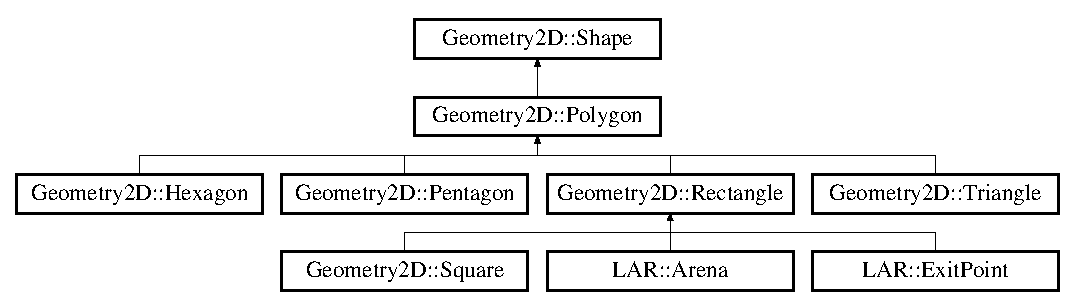
\includegraphics[height=3.684211cm]{class_geometry2_d_1_1_polygon}
\end{center}
\end{figure}
\subsection*{Public Member Functions}
\begin{DoxyCompactItemize}
\item 
\mbox{\Hypertarget{class_geometry2_d_1_1_polygon_a6b54a628e1da8663d7b5305ffbde5463}\label{class_geometry2_d_1_1_polygon_a6b54a628e1da8663d7b5305ffbde5463}} 
{\bfseries Polygon} (std\+::vector$<$ cv\+::\+Point $>$ \mbox{\hyperlink{class_geometry2_d_1_1_polygon_ab965e028324c2199022da00ff7eef14b}{points}})
\item 
\mbox{\Hypertarget{class_geometry2_d_1_1_polygon_a69276175f17a9a8c6171fdb5baaac778}\label{class_geometry2_d_1_1_polygon_a69276175f17a9a8c6171fdb5baaac778}} 
virtual void \mbox{\hyperlink{class_geometry2_d_1_1_polygon_a69276175f17a9a8c6171fdb5baaac778}{assign\+\_\+points}} ()=0
\begin{DoxyCompactList}\small\item\em assignes the points \end{DoxyCompactList}\item 
\mbox{\Hypertarget{class_geometry2_d_1_1_polygon_ae4a1f9df4b63affdce17f1926753ccd7}\label{class_geometry2_d_1_1_polygon_ae4a1f9df4b63affdce17f1926753ccd7}} 
void {\bfseries set\+Clipped\+Corners} (std\+::vector$<$ cv\+::\+Point $>$ \&\+\_\+clipped\+\_\+corners)
\item 
\mbox{\Hypertarget{class_geometry2_d_1_1_polygon_aedcccb53780e5f6cd49027200d35c370}\label{class_geometry2_d_1_1_polygon_aedcccb53780e5f6cd49027200d35c370}} 
std\+::vector$<$ cv\+::\+Point $>$ {\bfseries get\+Clipped\+Corners} ()
\end{DoxyCompactItemize}
\subsection*{Public Attributes}
\begin{DoxyCompactItemize}
\item 
\mbox{\Hypertarget{class_geometry2_d_1_1_polygon_ab965e028324c2199022da00ff7eef14b}\label{class_geometry2_d_1_1_polygon_ab965e028324c2199022da00ff7eef14b}} 
std\+::vector$<$ cv\+::\+Point $>$ \mbox{\hyperlink{class_geometry2_d_1_1_polygon_ab965e028324c2199022da00ff7eef14b}{points}}
\begin{DoxyCompactList}\small\item\em brief the points of the polygon \end{DoxyCompactList}\item 
\mbox{\Hypertarget{class_geometry2_d_1_1_polygon_a4260f5b694569381beb42bc9a1fffbcd}\label{class_geometry2_d_1_1_polygon_a4260f5b694569381beb42bc9a1fffbcd}} 
std\+::vector$<$ cv\+::\+Point $>$ {\bfseries clipped\+\_\+corners}
\end{DoxyCompactItemize}


The documentation for this class was generated from the following file\+:\begin{DoxyCompactItemize}
\item 
Polygon.\+hpp\end{DoxyCompactItemize}

\hypertarget{class_path2_d_1_1_element_1_1_position}{}\section{Path2D\+:\+:Element\+:\+:Position Class Reference}
\label{class_path2_d_1_1_element_1_1_position}\index{Path2\+D\+::\+Element\+::\+Position@{Path2\+D\+::\+Element\+::\+Position}}


describes a position of a point using x and y coordinates and orientation  




{\ttfamily \#include $<$Position.\+hpp$>$}

\subsection*{Public Member Functions}
\begin{DoxyCompactItemize}
\item 
\mbox{\Hypertarget{class_path2_d_1_1_element_1_1_position_aaa51dab67a1ef0a93f81f3357b07c403}\label{class_path2_d_1_1_element_1_1_position_aaa51dab67a1ef0a93f81f3357b07c403}} 
\mbox{\hyperlink{class_path2_d_1_1_element_1_1_position_aaa51dab67a1ef0a93f81f3357b07c403}{Position}} ()
\begin{DoxyCompactList}\small\item\em constructor of the \mbox{\hyperlink{class_path2_d_1_1_element_1_1_position}{Position}} class \end{DoxyCompactList}\item 
\mbox{\hyperlink{class_path2_d_1_1_element_1_1_position_ad8dafce9ad9442b93ebdb0d991f3b945}{Position}} (cv\+::\+Point2d pos, double orient)
\begin{DoxyCompactList}\small\item\em constructor of the \mbox{\hyperlink{class_path2_d_1_1_element_1_1_position}{Position}} class \end{DoxyCompactList}\item 
\mbox{\Hypertarget{class_path2_d_1_1_element_1_1_position_afd71b265ceb967ee9877bd45abc06a9a}\label{class_path2_d_1_1_element_1_1_position_afd71b265ceb967ee9877bd45abc06a9a}} 
\mbox{\hyperlink{class_path2_d_1_1_element_1_1_position_afd71b265ceb967ee9877bd45abc06a9a}{$\sim$\+Position}} ()
\begin{DoxyCompactList}\small\item\em destructor of the \mbox{\hyperlink{class_path2_d_1_1_element_1_1_position}{Position}} class \end{DoxyCompactList}\item 
void \mbox{\hyperlink{class_path2_d_1_1_element_1_1_position_ab0687fa319178000f2ee1f2d06e7c0df}{set\+Position}} (cv\+::\+Point2d position\+\_\+p, double orientation\+\_\+p)
\begin{DoxyCompactList}\small\item\em set the values of the position \end{DoxyCompactList}\item 
cv\+::\+Point2d \mbox{\hyperlink{class_path2_d_1_1_element_1_1_position_a02a5b758165848fe2f6a69e46904307f}{get\+Coordinates}} ()
\begin{DoxyCompactList}\small\item\em return the coordinates of the position \end{DoxyCompactList}\item 
double \mbox{\hyperlink{class_path2_d_1_1_element_1_1_position_ab40fecf77143ee106cbe1aa43d07a09d}{get\+Orientation}} ()
\begin{DoxyCompactList}\small\item\em return the orientation of the position \end{DoxyCompactList}\end{DoxyCompactItemize}
\subsection*{Public Attributes}
\begin{DoxyCompactItemize}
\item 
\mbox{\Hypertarget{class_path2_d_1_1_element_1_1_position_ab6dd50c899b47e8122ee9e6b89a8e9cf}\label{class_path2_d_1_1_element_1_1_position_ab6dd50c899b47e8122ee9e6b89a8e9cf}} 
bool {\bfseries orientation\+\_\+locked} = false
\item 
\mbox{\Hypertarget{class_path2_d_1_1_element_1_1_position_a1261c86b73661feef55e185e533ded5d}\label{class_path2_d_1_1_element_1_1_position_a1261c86b73661feef55e185e533ded5d}} 
double {\bfseries orientation}
\end{DoxyCompactItemize}


\subsection{Detailed Description}
describes a position of a point using x and y coordinates and orientation 

\subsection{Constructor \& Destructor Documentation}
\mbox{\Hypertarget{class_path2_d_1_1_element_1_1_position_ad8dafce9ad9442b93ebdb0d991f3b945}\label{class_path2_d_1_1_element_1_1_position_ad8dafce9ad9442b93ebdb0d991f3b945}} 
\index{Path2\+D\+::\+Element\+::\+Position@{Path2\+D\+::\+Element\+::\+Position}!Position@{Position}}
\index{Position@{Position}!Path2\+D\+::\+Element\+::\+Position@{Path2\+D\+::\+Element\+::\+Position}}
\subsubsection{\texorpdfstring{Position()}{Position()}}
{\footnotesize\ttfamily Path2\+D\+::\+Element\+::\+Position\+::\+Position (\begin{DoxyParamCaption}\item[{cv\+::\+Point2d}]{pos,  }\item[{double}]{orient }\end{DoxyParamCaption})}



constructor of the \mbox{\hyperlink{class_path2_d_1_1_element_1_1_position}{Position}} class 


\begin{DoxyParams}{Parameters}
{\em pos} & x and y coordinates \\
\hline
{\em orient} & orientation \\
\hline
\end{DoxyParams}


\subsection{Member Function Documentation}
\mbox{\Hypertarget{class_path2_d_1_1_element_1_1_position_a02a5b758165848fe2f6a69e46904307f}\label{class_path2_d_1_1_element_1_1_position_a02a5b758165848fe2f6a69e46904307f}} 
\index{Path2\+D\+::\+Element\+::\+Position@{Path2\+D\+::\+Element\+::\+Position}!get\+Coordinates@{get\+Coordinates}}
\index{get\+Coordinates@{get\+Coordinates}!Path2\+D\+::\+Element\+::\+Position@{Path2\+D\+::\+Element\+::\+Position}}
\subsubsection{\texorpdfstring{get\+Coordinates()}{getCoordinates()}}
{\footnotesize\ttfamily cv\+::\+Point2d Path2\+D\+::\+Element\+::\+Position\+::get\+Coordinates (\begin{DoxyParamCaption}{ }\end{DoxyParamCaption})}



return the coordinates of the position 

\begin{DoxyReturn}{Returns}
the coordinates of the position 
\end{DoxyReturn}
\mbox{\Hypertarget{class_path2_d_1_1_element_1_1_position_ab40fecf77143ee106cbe1aa43d07a09d}\label{class_path2_d_1_1_element_1_1_position_ab40fecf77143ee106cbe1aa43d07a09d}} 
\index{Path2\+D\+::\+Element\+::\+Position@{Path2\+D\+::\+Element\+::\+Position}!get\+Orientation@{get\+Orientation}}
\index{get\+Orientation@{get\+Orientation}!Path2\+D\+::\+Element\+::\+Position@{Path2\+D\+::\+Element\+::\+Position}}
\subsubsection{\texorpdfstring{get\+Orientation()}{getOrientation()}}
{\footnotesize\ttfamily double Path2\+D\+::\+Element\+::\+Position\+::get\+Orientation (\begin{DoxyParamCaption}{ }\end{DoxyParamCaption})}



return the orientation of the position 

\begin{DoxyReturn}{Returns}
the orientation of the position 
\end{DoxyReturn}
\mbox{\Hypertarget{class_path2_d_1_1_element_1_1_position_ab0687fa319178000f2ee1f2d06e7c0df}\label{class_path2_d_1_1_element_1_1_position_ab0687fa319178000f2ee1f2d06e7c0df}} 
\index{Path2\+D\+::\+Element\+::\+Position@{Path2\+D\+::\+Element\+::\+Position}!set\+Position@{set\+Position}}
\index{set\+Position@{set\+Position}!Path2\+D\+::\+Element\+::\+Position@{Path2\+D\+::\+Element\+::\+Position}}
\subsubsection{\texorpdfstring{set\+Position()}{setPosition()}}
{\footnotesize\ttfamily void Path2\+D\+::\+Element\+::\+Position\+::set\+Position (\begin{DoxyParamCaption}\item[{cv\+::\+Point2d}]{position\+\_\+p,  }\item[{double}]{orientation\+\_\+p }\end{DoxyParamCaption})}



set the values of the position 


\begin{DoxyParams}{Parameters}
{\em position\+\_\+p} & coordinates \\
\hline
{\em orientation\+\_\+p} & orientation \\
\hline
\end{DoxyParams}


The documentation for this class was generated from the following file\+:\begin{DoxyCompactItemize}
\item 
Position.\+hpp\end{DoxyCompactItemize}

\hypertarget{class_path2_d_1_1_dubin_path_finder_1_1_possible_dubin_path}{}\section{Path2D\+:\+:Dubin\+Path\+Finder\+:\+:Possible\+Dubin\+Path Class Reference}
\label{class_path2_d_1_1_dubin_path_finder_1_1_possible_dubin_path}\index{Path2\+D\+::\+Dubin\+Path\+Finder\+::\+Possible\+Dubin\+Path@{Path2\+D\+::\+Dubin\+Path\+Finder\+::\+Possible\+Dubin\+Path}}


class that describes a possible dubin path (useful during the calculation)  




{\ttfamily \#include $<$Dubin\+Path\+Finder.\+hpp$>$}

\subsection*{Public Member Functions}
\begin{DoxyCompactItemize}
\item 
\mbox{\Hypertarget{class_path2_d_1_1_dubin_path_finder_1_1_possible_dubin_path_a5ab9b2e9351f032edbadffa73f53318d}\label{class_path2_d_1_1_dubin_path_finder_1_1_possible_dubin_path_a5ab9b2e9351f032edbadffa73f53318d}} 
\mbox{\hyperlink{class_path2_d_1_1_dubin_path_finder_1_1_possible_dubin_path_a5ab9b2e9351f032edbadffa73f53318d}{Possible\+Dubin\+Path}} ()
\begin{DoxyCompactList}\small\item\em constructor of \mbox{\hyperlink{class_path2_d_1_1_dubin_path_finder_1_1_possible_dubin_path}{Possible\+Dubin\+Path}} class \end{DoxyCompactList}\item 
\mbox{\Hypertarget{class_path2_d_1_1_dubin_path_finder_1_1_possible_dubin_path_a0d7f0210884a2e9d4c24823d9b129b21}\label{class_path2_d_1_1_dubin_path_finder_1_1_possible_dubin_path_a0d7f0210884a2e9d4c24823d9b129b21}} 
\mbox{\hyperlink{class_path2_d_1_1_dubin_path_finder_1_1_possible_dubin_path_a0d7f0210884a2e9d4c24823d9b129b21}{$\sim$\+Possible\+Dubin\+Path}} ()
\begin{DoxyCompactList}\small\item\em destructor of \mbox{\hyperlink{class_path2_d_1_1_dubin_path_finder_1_1_possible_dubin_path}{Possible\+Dubin\+Path}} class \end{DoxyCompactList}\end{DoxyCompactItemize}
\subsection*{Public Attributes}
\begin{DoxyCompactItemize}
\item 
\mbox{\Hypertarget{class_path2_d_1_1_dubin_path_finder_1_1_possible_dubin_path_a6bd805f15b8e66169bd7c74edf4a8566}\label{class_path2_d_1_1_dubin_path_finder_1_1_possible_dubin_path_a6bd805f15b8e66169bd7c74edf4a8566}} 
bool {\bfseries ok}
\item 
\mbox{\Hypertarget{class_path2_d_1_1_dubin_path_finder_1_1_possible_dubin_path_a9c07bd6e2b9a01be56bd1a23b5c4e279}\label{class_path2_d_1_1_dubin_path_finder_1_1_possible_dubin_path_a9c07bd6e2b9a01be56bd1a23b5c4e279}} 
double {\bfseries sc\+\_\+s1}
\item 
\mbox{\Hypertarget{class_path2_d_1_1_dubin_path_finder_1_1_possible_dubin_path_a57c4d024385e0afa38b090667d42e151}\label{class_path2_d_1_1_dubin_path_finder_1_1_possible_dubin_path_a57c4d024385e0afa38b090667d42e151}} 
double {\bfseries sc\+\_\+s2}
\item 
\mbox{\Hypertarget{class_path2_d_1_1_dubin_path_finder_1_1_possible_dubin_path_a58a4eff149cbfff0af87ba29cc5440d3}\label{class_path2_d_1_1_dubin_path_finder_1_1_possible_dubin_path_a58a4eff149cbfff0af87ba29cc5440d3}} 
double {\bfseries sc\+\_\+s3}
\item 
\mbox{\Hypertarget{class_path2_d_1_1_dubin_path_finder_1_1_possible_dubin_path_a61c0e5502f74979e777d1d869a2edd9f}\label{class_path2_d_1_1_dubin_path_finder_1_1_possible_dubin_path_a61c0e5502f74979e777d1d869a2edd9f}} 
std\+::vector$<$ int $>$ {\bfseries signs}
\end{DoxyCompactItemize}


\subsection{Detailed Description}
class that describes a possible dubin path (useful during the calculation) 

The documentation for this class was generated from the following file\+:\begin{DoxyCompactItemize}
\item 
Dubin\+Path\+Finder.\+hpp\end{DoxyCompactItemize}

\hypertarget{class_geometry2_d_1_1_rectangle}{}\section{Geometry2D\+:\+:Rectangle Class Reference}
\label{class_geometry2_d_1_1_rectangle}\index{Geometry2\+D\+::\+Rectangle@{Geometry2\+D\+::\+Rectangle}}


Class for handling square in the map.  




{\ttfamily \#include $<$Rectangle.\+hpp$>$}

Inheritance diagram for Geometry2D\+:\+:Rectangle\+:\begin{figure}[H]
\begin{center}
\leavevmode
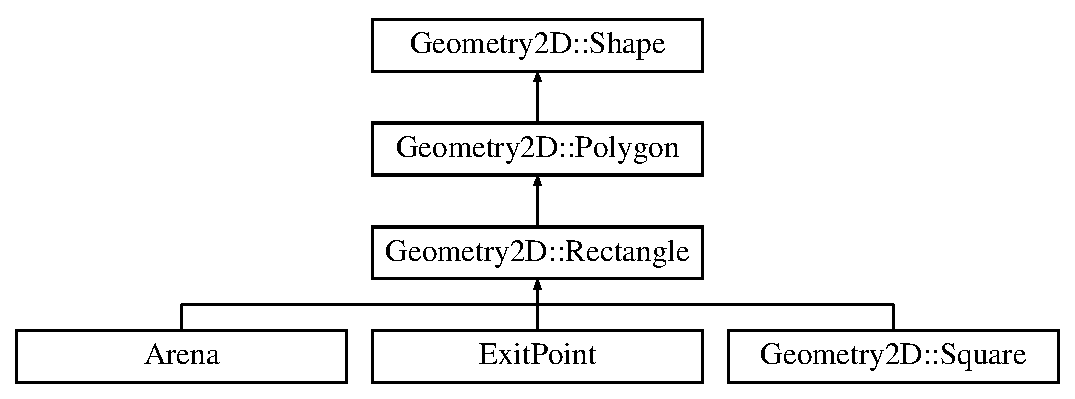
\includegraphics[height=4.000000cm]{class_geometry2_d_1_1_rectangle}
\end{center}
\end{figure}
\subsection*{Public Member Functions}
\begin{DoxyCompactItemize}
\item 
\mbox{\hyperlink{class_geometry2_d_1_1_rectangle_a2a2140f72054ed537c35bcd90bcdd593}{Rectangle}} ()
\item 
\mbox{\Hypertarget{class_geometry2_d_1_1_rectangle_a317593dc0f052818e86495ef1ec3b30e}\label{class_geometry2_d_1_1_rectangle_a317593dc0f052818e86495ef1ec3b30e}} 
{\bfseries Rectangle} (std\+::vector$<$ cv\+::\+Point $>$ \mbox{\hyperlink{class_geometry2_d_1_1_polygon_ab965e028324c2199022da00ff7eef14b}{points}})
\item 
\mbox{\hyperlink{class_geometry2_d_1_1_rectangle_a8fbc2f925d0b9e501cce72ec5282518a}{$\sim$\+Rectangle}} ()
\item 
std\+::vector$<$ cv\+::\+Point $>$ \mbox{\hyperlink{class_geometry2_d_1_1_rectangle_abe1ebd4b4d74c433120fdf9626a8dd65}{get\+Corners}} ()
\item 
void \mbox{\hyperlink{class_geometry2_d_1_1_rectangle_a5fc314db2e50e7b7b9360900d37ad212}{set\+Corners}} (std\+::vector$<$ cv\+::\+Point $>$ corners)
\item 
\mbox{\Hypertarget{class_geometry2_d_1_1_rectangle_a80d298e1dd64b46a6361f0f3d45fe0f7}\label{class_geometry2_d_1_1_rectangle_a80d298e1dd64b46a6361f0f3d45fe0f7}} 
cv\+::\+Point {\bfseries get\+Top\+Left} ()
\item 
\mbox{\Hypertarget{class_geometry2_d_1_1_rectangle_ac145e03588d1f1eb371f8547f7a6bd2d}\label{class_geometry2_d_1_1_rectangle_ac145e03588d1f1eb371f8547f7a6bd2d}} 
void {\bfseries set\+Top\+Left} (cv\+::\+Point top\+Left)
\item 
\mbox{\Hypertarget{class_geometry2_d_1_1_rectangle_af5b3d717ab45f875c7c36caa2dd38be7}\label{class_geometry2_d_1_1_rectangle_af5b3d717ab45f875c7c36caa2dd38be7}} 
cv\+::\+Point {\bfseries get\+Top\+Right} ()
\item 
\mbox{\Hypertarget{class_geometry2_d_1_1_rectangle_a00005d17343775c529a8cbacd0956bdb}\label{class_geometry2_d_1_1_rectangle_a00005d17343775c529a8cbacd0956bdb}} 
void {\bfseries set\+Top\+Right} (cv\+::\+Point top\+Right)
\item 
\mbox{\Hypertarget{class_geometry2_d_1_1_rectangle_ae07e78781178d09dd568e403e59517be}\label{class_geometry2_d_1_1_rectangle_ae07e78781178d09dd568e403e59517be}} 
cv\+::\+Point {\bfseries get\+Bottom\+Left} ()
\item 
\mbox{\Hypertarget{class_geometry2_d_1_1_rectangle_adbb3a9c4eabc748a1345447c48f7f39a}\label{class_geometry2_d_1_1_rectangle_adbb3a9c4eabc748a1345447c48f7f39a}} 
void {\bfseries set\+Bottom\+Left} (cv\+::\+Point bottom\+Left)
\item 
\mbox{\Hypertarget{class_geometry2_d_1_1_rectangle_a86f70f7f5fac9bdfc0e9b3d293ae6196}\label{class_geometry2_d_1_1_rectangle_a86f70f7f5fac9bdfc0e9b3d293ae6196}} 
cv\+::\+Point {\bfseries get\+Bottom\+Right} ()
\item 
\mbox{\Hypertarget{class_geometry2_d_1_1_rectangle_af037850b78e24d8588433fc877008ed3}\label{class_geometry2_d_1_1_rectangle_af037850b78e24d8588433fc877008ed3}} 
void {\bfseries set\+Bottom\+Right} (cv\+::\+Point bottom\+Right)
\item 
\mbox{\Hypertarget{class_geometry2_d_1_1_rectangle_ab4acb2a2f42304eed025b3efded350d0}\label{class_geometry2_d_1_1_rectangle_ab4acb2a2f42304eed025b3efded350d0}} 
void {\bfseries find\+Half} (int \&half\+\_\+h, int \&half\+\_\+w, const std\+::vector$<$ cv\+::\+Point $>$ \&corners)
\item 
\mbox{\Hypertarget{class_geometry2_d_1_1_rectangle_af9a483434ded2dac880fa682d2386dad}\label{class_geometry2_d_1_1_rectangle_af9a483434ded2dac880fa682d2386dad}} 
void \mbox{\hyperlink{class_geometry2_d_1_1_rectangle_af9a483434ded2dac880fa682d2386dad}{assign\+\_\+points}} ()
\begin{DoxyCompactList}\small\item\em assignes points to 1., 2., 3 etc point. \end{DoxyCompactList}\end{DoxyCompactItemize}
\subsection*{Public Attributes}
\begin{DoxyCompactItemize}
\item 
\mbox{\Hypertarget{class_geometry2_d_1_1_rectangle_aafa948683645e0038ff747cdbf7941e7}\label{class_geometry2_d_1_1_rectangle_aafa948683645e0038ff747cdbf7941e7}} 
cv\+::\+Point {\bfseries top\+\_\+left}
\item 
\mbox{\Hypertarget{class_geometry2_d_1_1_rectangle_a36c16fe3933944c63bfb3206363a37da}\label{class_geometry2_d_1_1_rectangle_a36c16fe3933944c63bfb3206363a37da}} 
cv\+::\+Point {\bfseries top\+\_\+right}
\item 
\mbox{\Hypertarget{class_geometry2_d_1_1_rectangle_ad7407dd1e39e1851c3474da1bde23ee0}\label{class_geometry2_d_1_1_rectangle_ad7407dd1e39e1851c3474da1bde23ee0}} 
cv\+::\+Point {\bfseries bottom\+\_\+left}
\item 
\mbox{\Hypertarget{class_geometry2_d_1_1_rectangle_ad7063cea41888253546f8f9d44dc4cd4}\label{class_geometry2_d_1_1_rectangle_ad7063cea41888253546f8f9d44dc4cd4}} 
cv\+::\+Point {\bfseries bottom\+\_\+right}
\end{DoxyCompactItemize}


\subsection{Detailed Description}
Class for handling square in the map. 

\subsection{Constructor \& Destructor Documentation}
\mbox{\Hypertarget{class_geometry2_d_1_1_rectangle_a2a2140f72054ed537c35bcd90bcdd593}\label{class_geometry2_d_1_1_rectangle_a2a2140f72054ed537c35bcd90bcdd593}} 
\index{Geometry2\+D\+::\+Rectangle@{Geometry2\+D\+::\+Rectangle}!Rectangle@{Rectangle}}
\index{Rectangle@{Rectangle}!Geometry2\+D\+::\+Rectangle@{Geometry2\+D\+::\+Rectangle}}
\subsubsection{\texorpdfstring{Rectangle()}{Rectangle()}}
{\footnotesize\ttfamily Geometry2\+D\+::\+Rectangle\+::\+Rectangle (\begin{DoxyParamCaption}{ }\end{DoxyParamCaption})}

constructor of square class \mbox{\Hypertarget{class_geometry2_d_1_1_rectangle_a8fbc2f925d0b9e501cce72ec5282518a}\label{class_geometry2_d_1_1_rectangle_a8fbc2f925d0b9e501cce72ec5282518a}} 
\index{Geometry2\+D\+::\+Rectangle@{Geometry2\+D\+::\+Rectangle}!````~Rectangle@{$\sim$\+Rectangle}}
\index{````~Rectangle@{$\sim$\+Rectangle}!Geometry2\+D\+::\+Rectangle@{Geometry2\+D\+::\+Rectangle}}
\subsubsection{\texorpdfstring{$\sim$\+Rectangle()}{~Rectangle()}}
{\footnotesize\ttfamily Geometry2\+D\+::\+Rectangle\+::$\sim$\+Rectangle (\begin{DoxyParamCaption}{ }\end{DoxyParamCaption})}

destructor of square class 

\subsection{Member Function Documentation}
\mbox{\Hypertarget{class_geometry2_d_1_1_rectangle_abe1ebd4b4d74c433120fdf9626a8dd65}\label{class_geometry2_d_1_1_rectangle_abe1ebd4b4d74c433120fdf9626a8dd65}} 
\index{Geometry2\+D\+::\+Rectangle@{Geometry2\+D\+::\+Rectangle}!get\+Corners@{get\+Corners}}
\index{get\+Corners@{get\+Corners}!Geometry2\+D\+::\+Rectangle@{Geometry2\+D\+::\+Rectangle}}
\subsubsection{\texorpdfstring{get\+Corners()}{getCorners()}}
{\footnotesize\ttfamily std\+::vector$<$cv\+::\+Point$>$ Geometry2\+D\+::\+Rectangle\+::get\+Corners (\begin{DoxyParamCaption}{ }\end{DoxyParamCaption})}

return the list of corners \begin{DoxyReturn}{Returns}
the list of corners 
\end{DoxyReturn}
\mbox{\Hypertarget{class_geometry2_d_1_1_rectangle_a5fc314db2e50e7b7b9360900d37ad212}\label{class_geometry2_d_1_1_rectangle_a5fc314db2e50e7b7b9360900d37ad212}} 
\index{Geometry2\+D\+::\+Rectangle@{Geometry2\+D\+::\+Rectangle}!set\+Corners@{set\+Corners}}
\index{set\+Corners@{set\+Corners}!Geometry2\+D\+::\+Rectangle@{Geometry2\+D\+::\+Rectangle}}
\subsubsection{\texorpdfstring{set\+Corners()}{setCorners()}}
{\footnotesize\ttfamily void Geometry2\+D\+::\+Rectangle\+::set\+Corners (\begin{DoxyParamCaption}\item[{std\+::vector$<$ cv\+::\+Point $>$}]{corners }\end{DoxyParamCaption})}


\begin{DoxyParams}{Parameters}
{\em corners} & return the list of corners \\
\hline
\end{DoxyParams}


The documentation for this class was generated from the following file\+:\begin{DoxyCompactItemize}
\item 
Rectangle.\+hpp\end{DoxyCompactItemize}

\hypertarget{class_robot}{}\section{Robot Class Reference}
\label{class_robot}\index{Robot@{Robot}}
Inheritance diagram for Robot\+:\begin{figure}[H]
\begin{center}
\leavevmode
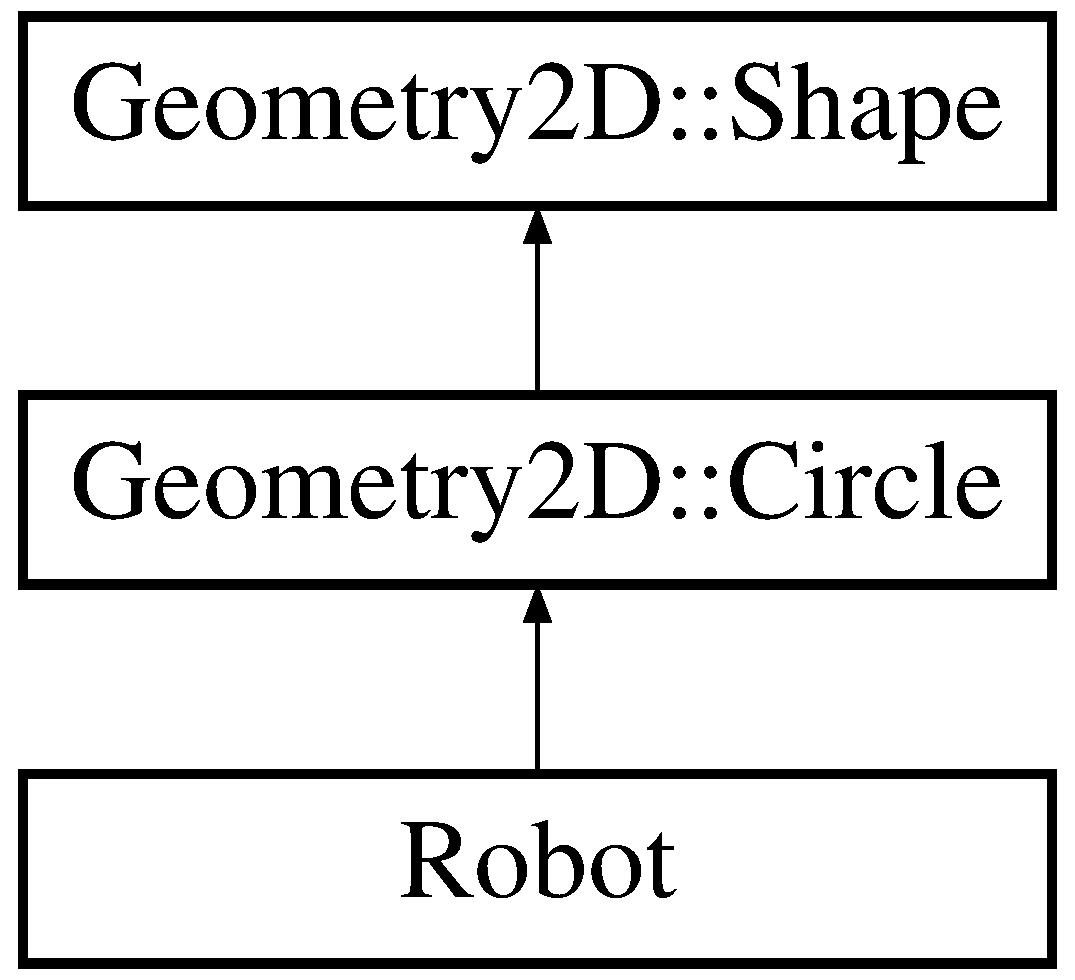
\includegraphics[height=3.000000cm]{class_robot}
\end{center}
\end{figure}
\subsection*{Public Member Functions}
\begin{DoxyCompactItemize}
\item 
\mbox{\Hypertarget{class_robot_a80c1083dea6724f840e7900210359f2a}\label{class_robot_a80c1083dea6724f840e7900210359f2a}} 
\mbox{\hyperlink{class_path_coordinates}{Path\+Coordinates}} {\bfseries initialize} ()
\end{DoxyCompactItemize}
\subsection*{Public Attributes}
\begin{DoxyCompactItemize}
\item 
\mbox{\Hypertarget{class_robot_a8f89b1b5df8f5e247e608787923fe06c}\label{class_robot_a8f89b1b5df8f5e247e608787923fe06c}} 
const cv\+::\+Scalar {\bfseries color} = cv\+::\+Scalar(0,0,255)
\item 
\mbox{\Hypertarget{class_robot_a0bda826aa4ed4fd9508fdbe02648d123}\label{class_robot_a0bda826aa4ed4fd9508fdbe02648d123}} 
\mbox{\hyperlink{class_path_coordinates}{Path\+Coordinates}} $\ast$ {\bfseries data}
\end{DoxyCompactItemize}


The documentation for this class was generated from the following file\+:\begin{DoxyCompactItemize}
\item 
Robot.\+hpp\end{DoxyCompactItemize}

\hypertarget{class_settings}{}\section{Settings Class Reference}
\label{class_settings}\index{Settings@{Settings}}
\subsection*{Public Types}
\begin{DoxyCompactItemize}
\item 
\mbox{\Hypertarget{class_settings_a0e7117abd9427a6f8bc1d1d8d456b5c8}\label{class_settings_a0e7117abd9427a6f8bc1d1d8d456b5c8}} 
enum {\bfseries Pattern} \{ {\bfseries N\+O\+T\+\_\+\+E\+X\+I\+S\+T\+I\+NG}, 
{\bfseries C\+H\+E\+S\+S\+B\+O\+A\+RD}, 
{\bfseries C\+I\+R\+C\+L\+E\+S\+\_\+\+G\+R\+ID}, 
{\bfseries A\+S\+Y\+M\+M\+E\+T\+R\+I\+C\+\_\+\+C\+I\+R\+C\+L\+E\+S\+\_\+\+G\+R\+ID}
 \}
\item 
\mbox{\Hypertarget{class_settings_a5afe85d24b071973a7f248c05386f7f4}\label{class_settings_a5afe85d24b071973a7f248c05386f7f4}} 
enum {\bfseries Input\+Type} \{ {\bfseries I\+N\+V\+A\+L\+ID}, 
{\bfseries C\+A\+M\+E\+RA}, 
{\bfseries V\+I\+D\+E\+O\+\_\+\+F\+I\+LE}, 
{\bfseries I\+M\+A\+G\+E\+\_\+\+L\+I\+ST}
 \}
\end{DoxyCompactItemize}
\subsection*{Public Member Functions}
\begin{DoxyCompactItemize}
\item 
\mbox{\Hypertarget{class_settings_a0785cc2055091b2a857b1dcefe291acc}\label{class_settings_a0785cc2055091b2a857b1dcefe291acc}} 
void {\bfseries write} (File\+Storage \&fs) const
\item 
\mbox{\Hypertarget{class_settings_a2d7841f8441095032e0f3b7d20adfd3f}\label{class_settings_a2d7841f8441095032e0f3b7d20adfd3f}} 
void {\bfseries read} (const File\+Node \&node)
\item 
\mbox{\Hypertarget{class_settings_a29016205c90b95d6247df18365a70dd0}\label{class_settings_a29016205c90b95d6247df18365a70dd0}} 
void {\bfseries validate} ()
\item 
\mbox{\Hypertarget{class_settings_a7701462e928f2425b342440fba9973e5}\label{class_settings_a7701462e928f2425b342440fba9973e5}} 
Mat {\bfseries next\+Image} ()
\end{DoxyCompactItemize}
\subsection*{Static Public Member Functions}
\begin{DoxyCompactItemize}
\item 
\mbox{\Hypertarget{class_settings_a67f01f62ca469d9ed75794079eb53c9d}\label{class_settings_a67f01f62ca469d9ed75794079eb53c9d}} 
static bool {\bfseries read\+String\+List} (const std\+::string \&filename, std\+::vector$<$ std\+::string $>$ \&l)
\item 
\mbox{\Hypertarget{class_settings_aa69f25fc79fe1dd05d990dade16669ea}\label{class_settings_aa69f25fc79fe1dd05d990dade16669ea}} 
static bool {\bfseries is\+List\+Of\+Images} (const std\+::string \&filename)
\end{DoxyCompactItemize}
\subsection*{Public Attributes}
\begin{DoxyCompactItemize}
\item 
\mbox{\Hypertarget{class_settings_a5030a7164df923bb3b86dd7a0fc9af30}\label{class_settings_a5030a7164df923bb3b86dd7a0fc9af30}} 
Size {\bfseries board\+Size}
\item 
\mbox{\Hypertarget{class_settings_a94551b7ffe8ac60311b035b2905e9498}\label{class_settings_a94551b7ffe8ac60311b035b2905e9498}} 
Pattern {\bfseries calibration\+Pattern}
\item 
\mbox{\Hypertarget{class_settings_a6c94708776ad1ce258fc44f2101f5941}\label{class_settings_a6c94708776ad1ce258fc44f2101f5941}} 
float {\bfseries square\+Size}
\item 
\mbox{\Hypertarget{class_settings_a7e6654cd0e51791ed687eaa85f8fc143}\label{class_settings_a7e6654cd0e51791ed687eaa85f8fc143}} 
int {\bfseries nr\+Frames}
\item 
\mbox{\Hypertarget{class_settings_af55c910308a0d773055d0b19261bb3b8}\label{class_settings_af55c910308a0d773055d0b19261bb3b8}} 
float {\bfseries aspect\+Ratio}
\item 
\mbox{\Hypertarget{class_settings_a5fe947366441009187d633f9e4663256}\label{class_settings_a5fe947366441009187d633f9e4663256}} 
int {\bfseries delay}
\item 
\mbox{\Hypertarget{class_settings_a53ac449815682c6bfae7e50944ba0565}\label{class_settings_a53ac449815682c6bfae7e50944ba0565}} 
bool {\bfseries write\+Points}
\item 
\mbox{\Hypertarget{class_settings_a1cee56847e08f49c90d2f7e2b0511197}\label{class_settings_a1cee56847e08f49c90d2f7e2b0511197}} 
bool {\bfseries write\+Extrinsics}
\item 
\mbox{\Hypertarget{class_settings_a4bc7ff147d74721a3587ce6fcb64ef32}\label{class_settings_a4bc7ff147d74721a3587ce6fcb64ef32}} 
bool {\bfseries calib\+Zero\+Tangent\+Dist}
\item 
\mbox{\Hypertarget{class_settings_a44397eea3f08a0c78808c38bdd716594}\label{class_settings_a44397eea3f08a0c78808c38bdd716594}} 
bool {\bfseries calib\+Fix\+Principal\+Point}
\item 
\mbox{\Hypertarget{class_settings_ab6304f260b315d2820f755e1c3a052b5}\label{class_settings_ab6304f260b315d2820f755e1c3a052b5}} 
bool {\bfseries flip\+Vertical}
\item 
\mbox{\Hypertarget{class_settings_ab2fec20428d21ea867cc044c0a583cf1}\label{class_settings_ab2fec20428d21ea867cc044c0a583cf1}} 
std\+::string {\bfseries output\+File\+Name}
\item 
\mbox{\Hypertarget{class_settings_a935d6f27ee454e9fee63f8b662f48a06}\label{class_settings_a935d6f27ee454e9fee63f8b662f48a06}} 
bool {\bfseries show\+Undistorsed}
\item 
\mbox{\Hypertarget{class_settings_a8696deae231b0efe48f1d069a4145ee6}\label{class_settings_a8696deae231b0efe48f1d069a4145ee6}} 
std\+::string {\bfseries input}
\item 
\mbox{\Hypertarget{class_settings_ac8f271630d54f9d0c718ea0130972d44}\label{class_settings_ac8f271630d54f9d0c718ea0130972d44}} 
bool {\bfseries use\+Fisheye}
\item 
\mbox{\Hypertarget{class_settings_a25242813ee2c5e111ce48fe1f7f85e7b}\label{class_settings_a25242813ee2c5e111ce48fe1f7f85e7b}} 
bool {\bfseries fix\+K1}
\item 
\mbox{\Hypertarget{class_settings_abad0b643dc5a39d493a6343d38f41578}\label{class_settings_abad0b643dc5a39d493a6343d38f41578}} 
bool {\bfseries fix\+K2}
\item 
\mbox{\Hypertarget{class_settings_a433fca3c377d42f1c7d43e35a286913f}\label{class_settings_a433fca3c377d42f1c7d43e35a286913f}} 
bool {\bfseries fix\+K3}
\item 
\mbox{\Hypertarget{class_settings_ac993998a56cebe0593cb74fe39858d31}\label{class_settings_ac993998a56cebe0593cb74fe39858d31}} 
bool {\bfseries fix\+K4}
\item 
\mbox{\Hypertarget{class_settings_a4d0d37eef5f3033a8aabc3f09ee29a03}\label{class_settings_a4d0d37eef5f3033a8aabc3f09ee29a03}} 
bool {\bfseries fix\+K5}
\item 
\mbox{\Hypertarget{class_settings_af32a5ff06192bde106c934e0361bcd7e}\label{class_settings_af32a5ff06192bde106c934e0361bcd7e}} 
int {\bfseries camera\+ID}
\item 
\mbox{\Hypertarget{class_settings_ab3f8f916639b93c3b5079facfe395078}\label{class_settings_ab3f8f916639b93c3b5079facfe395078}} 
std\+::vector$<$ std\+::string $>$ {\bfseries image\+List}
\item 
\mbox{\Hypertarget{class_settings_a1b89e85a2638e19f2d53269245d19b66}\label{class_settings_a1b89e85a2638e19f2d53269245d19b66}} 
size\+\_\+t {\bfseries at\+Image\+List}
\item 
\mbox{\Hypertarget{class_settings_abd5706146b34d3c32aef4025dcd2ec1b}\label{class_settings_abd5706146b34d3c32aef4025dcd2ec1b}} 
Video\+Capture {\bfseries input\+Capture}
\item 
\mbox{\Hypertarget{class_settings_a89fb14ce9856fb642f18bb0f7c5b8868}\label{class_settings_a89fb14ce9856fb642f18bb0f7c5b8868}} 
Input\+Type {\bfseries input\+Type}
\item 
\mbox{\Hypertarget{class_settings_a3b9fc27b555f982bd5b9ea5198e1f7e3}\label{class_settings_a3b9fc27b555f982bd5b9ea5198e1f7e3}} 
bool {\bfseries good\+Input}
\item 
\mbox{\Hypertarget{class_settings_aba5691e3e76525f93ea254e654ec3717}\label{class_settings_aba5691e3e76525f93ea254e654ec3717}} 
int {\bfseries flag}
\end{DoxyCompactItemize}


The documentation for this class was generated from the following file\+:\begin{DoxyCompactItemize}
\item 
Settings.\+hpp\end{DoxyCompactItemize}

\hypertarget{class_geometry2_d_1_1_shape}{}\section{Geometry2D\+:\+:Shape Class Reference}
\label{class_geometry2_d_1_1_shape}\index{Geometry2\+D\+::\+Shape@{Geometry2\+D\+::\+Shape}}


class for handling all the shapes in the map  




{\ttfamily \#include $<$Shape.\+hpp$>$}

Inheritance diagram for Geometry2D\+:\+:Shape\+:\begin{figure}[H]
\begin{center}
\leavevmode
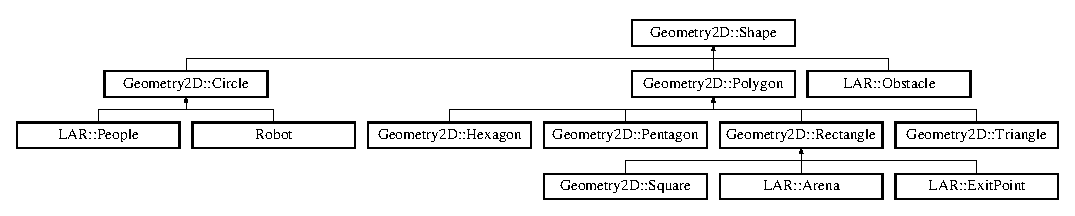
\includegraphics[height=2.456141cm]{class_geometry2_d_1_1_shape}
\end{center}
\end{figure}
\subsection*{Public Member Functions}
\begin{DoxyCompactItemize}
\item 
\mbox{\hyperlink{class_geometry2_d_1_1_shape_a22028a42d94c013c15909c2601ace514}{Shape}} ()
\item 
\mbox{\hyperlink{class_geometry2_d_1_1_shape_ad475fc843313521e75906737ecd7f459}{$\sim$\+Shape}} ()
\item 
void \mbox{\hyperlink{class_geometry2_d_1_1_shape_a25ec0d592589f6205012c84828b33fb3}{set\+Cell}} (\mbox{\hyperlink{class_cell}{Cell}} \&cell\+\_\+i)
\item 
std\+::vector$<$ \mbox{\hyperlink{class_cell}{Cell}} $\ast$ $>$ \mbox{\hyperlink{class_geometry2_d_1_1_shape_a561811570c6e3efd024a048556ca370f}{get\+Cell}} ()
\end{DoxyCompactItemize}


\subsection{Detailed Description}
class for handling all the shapes in the map 

\subsection{Constructor \& Destructor Documentation}
\mbox{\Hypertarget{class_geometry2_d_1_1_shape_a22028a42d94c013c15909c2601ace514}\label{class_geometry2_d_1_1_shape_a22028a42d94c013c15909c2601ace514}} 
\index{Geometry2\+D\+::\+Shape@{Geometry2\+D\+::\+Shape}!Shape@{Shape}}
\index{Shape@{Shape}!Geometry2\+D\+::\+Shape@{Geometry2\+D\+::\+Shape}}
\subsubsection{\texorpdfstring{Shape()}{Shape()}}
{\footnotesize\ttfamily Geometry2\+D\+::\+Shape\+::\+Shape (\begin{DoxyParamCaption}{ }\end{DoxyParamCaption})}

constructor of the shape class \mbox{\Hypertarget{class_geometry2_d_1_1_shape_ad475fc843313521e75906737ecd7f459}\label{class_geometry2_d_1_1_shape_ad475fc843313521e75906737ecd7f459}} 
\index{Geometry2\+D\+::\+Shape@{Geometry2\+D\+::\+Shape}!````~Shape@{$\sim$\+Shape}}
\index{````~Shape@{$\sim$\+Shape}!Geometry2\+D\+::\+Shape@{Geometry2\+D\+::\+Shape}}
\subsubsection{\texorpdfstring{$\sim$\+Shape()}{~Shape()}}
{\footnotesize\ttfamily Geometry2\+D\+::\+Shape\+::$\sim$\+Shape (\begin{DoxyParamCaption}{ }\end{DoxyParamCaption})}

destructor of the shape class 

\subsection{Member Function Documentation}
\mbox{\Hypertarget{class_geometry2_d_1_1_shape_a561811570c6e3efd024a048556ca370f}\label{class_geometry2_d_1_1_shape_a561811570c6e3efd024a048556ca370f}} 
\index{Geometry2\+D\+::\+Shape@{Geometry2\+D\+::\+Shape}!get\+Cell@{get\+Cell}}
\index{get\+Cell@{get\+Cell}!Geometry2\+D\+::\+Shape@{Geometry2\+D\+::\+Shape}}
\subsubsection{\texorpdfstring{get\+Cell()}{getCell()}}
{\footnotesize\ttfamily std\+::vector$<$\mbox{\hyperlink{class_cell}{Cell}}$\ast$$>$ Geometry2\+D\+::\+Shape\+::get\+Cell (\begin{DoxyParamCaption}{ }\end{DoxyParamCaption})}

return the cell which is connected \begin{DoxyReturn}{Returns}
the cell which is connected 
\end{DoxyReturn}
\mbox{\Hypertarget{class_geometry2_d_1_1_shape_a25ec0d592589f6205012c84828b33fb3}\label{class_geometry2_d_1_1_shape_a25ec0d592589f6205012c84828b33fb3}} 
\index{Geometry2\+D\+::\+Shape@{Geometry2\+D\+::\+Shape}!set\+Cell@{set\+Cell}}
\index{set\+Cell@{set\+Cell}!Geometry2\+D\+::\+Shape@{Geometry2\+D\+::\+Shape}}
\subsubsection{\texorpdfstring{set\+Cell()}{setCell()}}
{\footnotesize\ttfamily void Geometry2\+D\+::\+Shape\+::set\+Cell (\begin{DoxyParamCaption}\item[{\mbox{\hyperlink{class_cell}{Cell}} \&}]{cell\+\_\+i }\end{DoxyParamCaption})}

connect a cell to the shape 
\begin{DoxyParams}{Parameters}
{\em cell\+\_\+i} & cell that has to be connected to the shape \\
\hline
\end{DoxyParams}


The documentation for this class was generated from the following file\+:\begin{DoxyCompactItemize}
\item 
Shape.\+hpp\end{DoxyCompactItemize}

\hypertarget{class_geometry2_d_1_1_square}{}\section{Geometry2D\+:\+:Square Class Reference}
\label{class_geometry2_d_1_1_square}\index{Geometry2\+D\+::\+Square@{Geometry2\+D\+::\+Square}}


A \mbox{\hyperlink{class_geometry2_d_1_1_shape}{Shape}} type similar to a \mbox{\hyperlink{class_geometry2_d_1_1_rectangle}{Rectangle}} but with equdistant lengths.  




{\ttfamily \#include $<$Square.\+hpp$>$}

Inheritance diagram for Geometry2D\+:\+:Square\+:\begin{figure}[H]
\begin{center}
\leavevmode
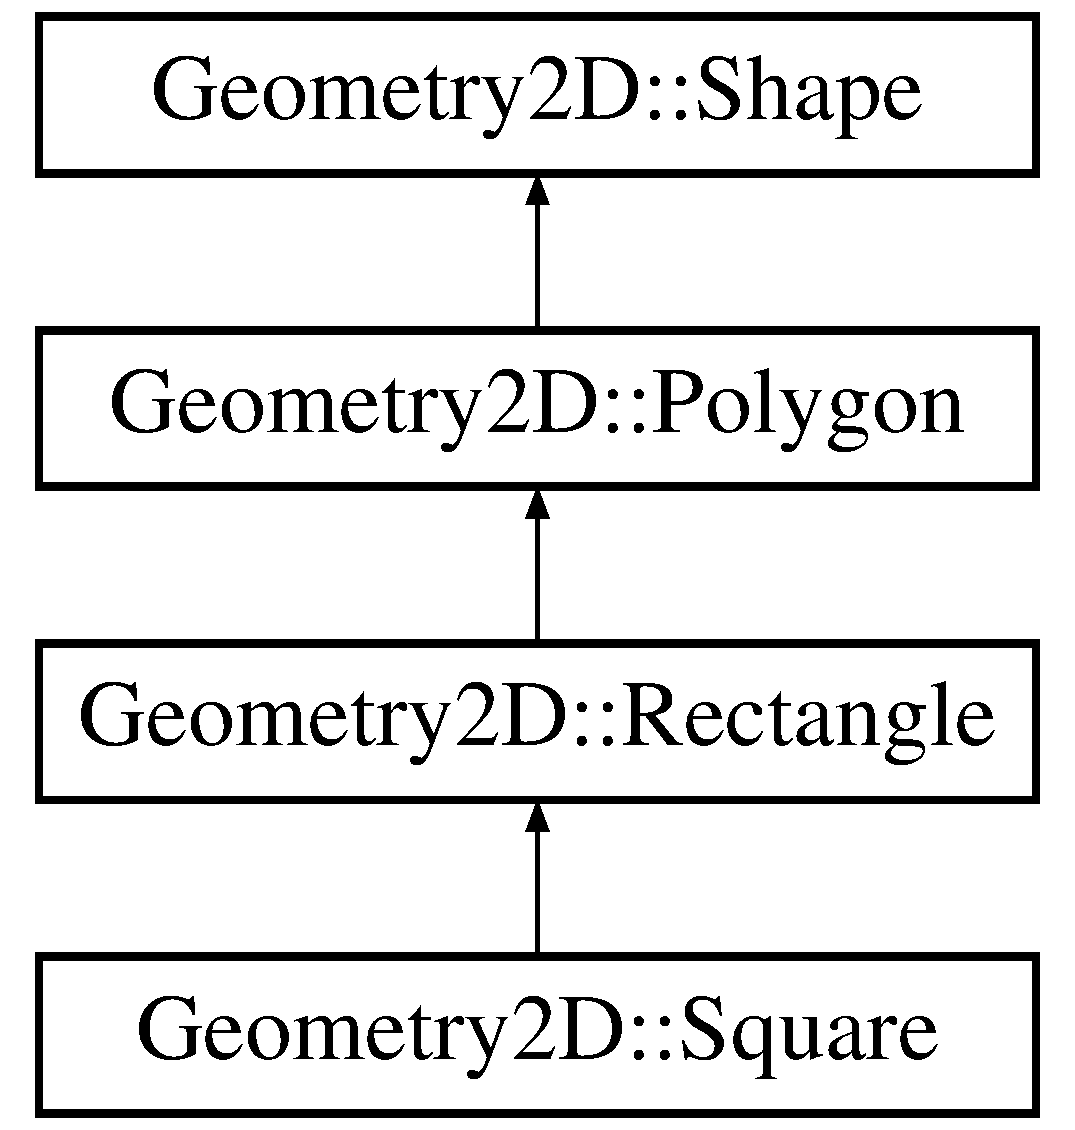
\includegraphics[height=4.000000cm]{class_geometry2_d_1_1_square}
\end{center}
\end{figure}
\subsection*{Additional Inherited Members}


\subsection{Detailed Description}
A \mbox{\hyperlink{class_geometry2_d_1_1_shape}{Shape}} type similar to a \mbox{\hyperlink{class_geometry2_d_1_1_rectangle}{Rectangle}} but with equdistant lengths. 

The documentation for this class was generated from the following file\+:\begin{DoxyCompactItemize}
\item 
Square.\+hpp\end{DoxyCompactItemize}

\hypertarget{struct_path2_d_1_1_dubin_path_finder_1_1standard_conf}{}\section{Path2D\+:\+:Dubin\+Path\+Finder\+:\+:standard\+Conf Struct Reference}
\label{struct_path2_d_1_1_dubin_path_finder_1_1standard_conf}\index{Path2\+D\+::\+Dubin\+Path\+Finder\+::standard\+Conf@{Path2\+D\+::\+Dubin\+Path\+Finder\+::standard\+Conf}}
\subsection*{Public Attributes}
\begin{DoxyCompactItemize}
\item 
\mbox{\Hypertarget{struct_path2_d_1_1_dubin_path_finder_1_1standard_conf_a6383aeef4501ac4b4c31006f84cb801b}\label{struct_path2_d_1_1_dubin_path_finder_1_1standard_conf_a6383aeef4501ac4b4c31006f84cb801b}} 
double {\bfseries lambda}
\item 
\mbox{\Hypertarget{struct_path2_d_1_1_dubin_path_finder_1_1standard_conf_a78e4fe8bea873cb8deb9b54435e6d880}\label{struct_path2_d_1_1_dubin_path_finder_1_1standard_conf_a78e4fe8bea873cb8deb9b54435e6d880}} 
double {\bfseries sc\+\_\+th0}
\item 
\mbox{\Hypertarget{struct_path2_d_1_1_dubin_path_finder_1_1standard_conf_a4dc3e36105b402b5835644443b86e9de}\label{struct_path2_d_1_1_dubin_path_finder_1_1standard_conf_a4dc3e36105b402b5835644443b86e9de}} 
double {\bfseries sc\+\_\+thf}
\item 
\mbox{\Hypertarget{struct_path2_d_1_1_dubin_path_finder_1_1standard_conf_a3895d6f2dd23fefcc3bad68f2e65a05f}\label{struct_path2_d_1_1_dubin_path_finder_1_1standard_conf_a3895d6f2dd23fefcc3bad68f2e65a05f}} 
double {\bfseries sc\+\_\+\+Kmax}
\end{DoxyCompactItemize}


The documentation for this struct was generated from the following file\+:\begin{DoxyCompactItemize}
\item 
Dubin\+Path\+Finder.\+hpp\end{DoxyCompactItemize}

\hypertarget{class_path2_d_1_1_element_1_1_straight_line}{}\section{Path2D\+:\+:Element\+:\+:Straight\+Line Class Reference}
\label{class_path2_d_1_1_element_1_1_straight_line}\index{Path2\+D\+::\+Element\+::\+Straight\+Line@{Path2\+D\+::\+Element\+::\+Straight\+Line}}


describe a \mbox{\hyperlink{class_path2_d_1_1_element_1_1_straight_line}{Straight\+Line}} in the path  




{\ttfamily \#include $<$Straight\+Line.\+hpp$>$}

Inheritance diagram for Path2D\+:\+:Element\+:\+:Straight\+Line\+:\begin{figure}[H]
\begin{center}
\leavevmode
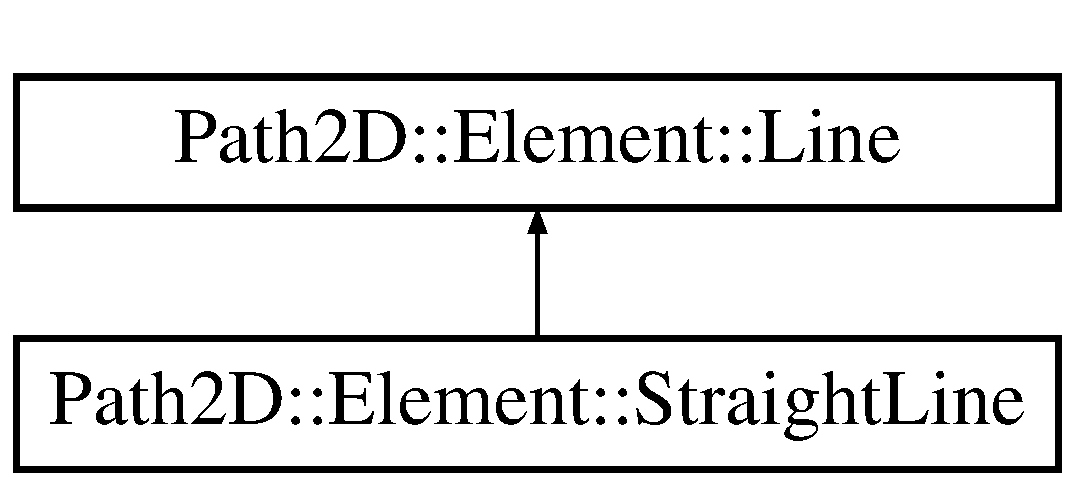
\includegraphics[height=2.000000cm]{class_path2_d_1_1_element_1_1_straight_line}
\end{center}
\end{figure}
\subsection*{Public Member Functions}
\begin{DoxyCompactItemize}
\item 
\mbox{\hyperlink{class_path2_d_1_1_element_1_1_straight_line_a831171d36fe596a4b891d9db7c513af6}{Straight\+Line}} (\mbox{\hyperlink{class_path2_d_1_1_element_1_1_position}{Position}} start\+\_\+point, \mbox{\hyperlink{class_path2_d_1_1_element_1_1_position}{Position}} end\+\_\+point)
\begin{DoxyCompactList}\small\item\em constructor of the \mbox{\hyperlink{class_path2_d_1_1_element_1_1_straight_line}{Straight\+Line}} class \end{DoxyCompactList}\item 
\mbox{\hyperlink{class_path2_d_1_1_element_1_1_straight_line_a618128b2e4005f9671d55165ddc114de}{Straight\+Line}} (\mbox{\hyperlink{class_path2_d_1_1_element_1_1_position}{Position}} start\+\_\+point, double length)
\begin{DoxyCompactList}\small\item\em constructor of the \mbox{\hyperlink{class_path2_d_1_1_element_1_1_straight_line}{Straight\+Line}} class \end{DoxyCompactList}\item 
\mbox{\Hypertarget{class_path2_d_1_1_element_1_1_straight_line_a5b61a97e2f0b06ecf09b534fcfc645f3}\label{class_path2_d_1_1_element_1_1_straight_line_a5b61a97e2f0b06ecf09b534fcfc645f3}} 
\mbox{\hyperlink{class_path2_d_1_1_element_1_1_straight_line_a5b61a97e2f0b06ecf09b534fcfc645f3}{$\sim$\+Straight\+Line}} ()
\begin{DoxyCompactList}\small\item\em destructor of the \mbox{\hyperlink{class_path2_d_1_1_element_1_1_straight_line}{Straight\+Line}} class \end{DoxyCompactList}\end{DoxyCompactItemize}


\subsection{Detailed Description}
describe a \mbox{\hyperlink{class_path2_d_1_1_element_1_1_straight_line}{Straight\+Line}} in the path 

\subsection{Constructor \& Destructor Documentation}
\mbox{\Hypertarget{class_path2_d_1_1_element_1_1_straight_line_a831171d36fe596a4b891d9db7c513af6}\label{class_path2_d_1_1_element_1_1_straight_line_a831171d36fe596a4b891d9db7c513af6}} 
\index{Path2\+D\+::\+Element\+::\+Straight\+Line@{Path2\+D\+::\+Element\+::\+Straight\+Line}!Straight\+Line@{Straight\+Line}}
\index{Straight\+Line@{Straight\+Line}!Path2\+D\+::\+Element\+::\+Straight\+Line@{Path2\+D\+::\+Element\+::\+Straight\+Line}}
\subsubsection{\texorpdfstring{Straight\+Line()}{StraightLine()}\hspace{0.1cm}{\footnotesize\ttfamily [1/2]}}
{\footnotesize\ttfamily Path2\+D\+::\+Element\+::\+Straight\+Line\+::\+Straight\+Line (\begin{DoxyParamCaption}\item[{\mbox{\hyperlink{class_path2_d_1_1_element_1_1_position}{Position}}}]{start\+\_\+point,  }\item[{\mbox{\hyperlink{class_path2_d_1_1_element_1_1_position}{Position}}}]{end\+\_\+point }\end{DoxyParamCaption})}



constructor of the \mbox{\hyperlink{class_path2_d_1_1_element_1_1_straight_line}{Straight\+Line}} class 


\begin{DoxyParams}{Parameters}
{\em start\+\_\+point} & start point of the line \\
\hline
{\em end\+\_\+point} & end point of the line \\
\hline
\end{DoxyParams}
\mbox{\Hypertarget{class_path2_d_1_1_element_1_1_straight_line_a618128b2e4005f9671d55165ddc114de}\label{class_path2_d_1_1_element_1_1_straight_line_a618128b2e4005f9671d55165ddc114de}} 
\index{Path2\+D\+::\+Element\+::\+Straight\+Line@{Path2\+D\+::\+Element\+::\+Straight\+Line}!Straight\+Line@{Straight\+Line}}
\index{Straight\+Line@{Straight\+Line}!Path2\+D\+::\+Element\+::\+Straight\+Line@{Path2\+D\+::\+Element\+::\+Straight\+Line}}
\subsubsection{\texorpdfstring{Straight\+Line()}{StraightLine()}\hspace{0.1cm}{\footnotesize\ttfamily [2/2]}}
{\footnotesize\ttfamily Path2\+D\+::\+Element\+::\+Straight\+Line\+::\+Straight\+Line (\begin{DoxyParamCaption}\item[{\mbox{\hyperlink{class_path2_d_1_1_element_1_1_position}{Position}}}]{start\+\_\+point,  }\item[{double}]{length }\end{DoxyParamCaption})}



constructor of the \mbox{\hyperlink{class_path2_d_1_1_element_1_1_straight_line}{Straight\+Line}} class 


\begin{DoxyParams}{Parameters}
{\em start\+\_\+point} & start point of the line \\
\hline
{\em length} & length of the line \\
\hline
\end{DoxyParams}


The documentation for this class was generated from the following file\+:\begin{DoxyCompactItemize}
\item 
Straight\+Line.\+hpp\end{DoxyCompactItemize}

\hypertarget{class_image_processing_1_1_template___character___recognition}{}\section{Image\+Processing\+:\+:Template\+\_\+\+Character\+\_\+\+Recognition Class Reference}
\label{class_image_processing_1_1_template___character___recognition}\index{Image\+Processing\+::\+Template\+\_\+\+Character\+\_\+\+Recognition@{Image\+Processing\+::\+Template\+\_\+\+Character\+\_\+\+Recognition}}


Class that performs the Template Matching Method to identify characters.  




{\ttfamily \#include $<$Template\+\_\+\+Character\+\_\+\+Recognition.\+hpp$>$}

Inheritance diagram for Image\+Processing\+:\+:Template\+\_\+\+Character\+\_\+\+Recognition\+:\begin{figure}[H]
\begin{center}
\leavevmode
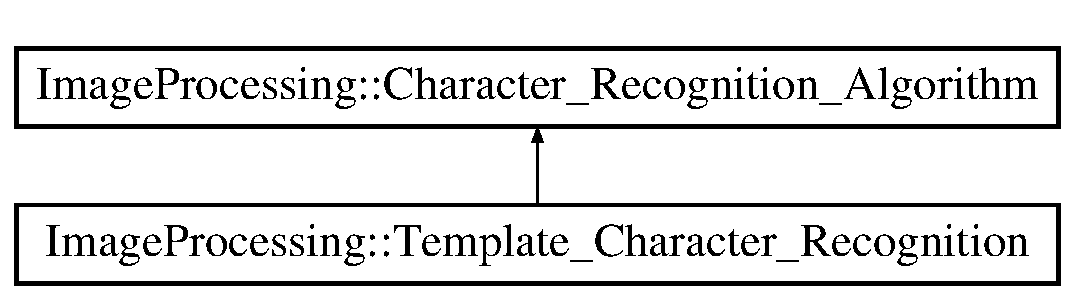
\includegraphics[height=2.000000cm]{class_image_processing_1_1_template___character___recognition}
\end{center}
\end{figure}
\subsection*{Public Member Functions}
\begin{DoxyCompactItemize}
\item 
\mbox{\Hypertarget{class_image_processing_1_1_template___character___recognition_a70b7337f493c829d8e5879b75bc98342}\label{class_image_processing_1_1_template___character___recognition_a70b7337f493c829d8e5879b75bc98342}} 
std\+::pair$<$ int, int $>$ \mbox{\hyperlink{class_image_processing_1_1_template___character___recognition_a70b7337f493c829d8e5879b75bc98342}{detect\+\_\+digit}} (cv\+::\+Mat \&image)
\begin{DoxyCompactList}\small\item\em detect a digit in a prepared image \end{DoxyCompactList}\end{DoxyCompactItemize}
\subsection*{Public Attributes}
\begin{DoxyCompactItemize}
\item 
\mbox{\Hypertarget{class_image_processing_1_1_template___character___recognition_a2f7756520ceae78af0715328c70221b9}\label{class_image_processing_1_1_template___character___recognition_a2f7756520ceae78af0715328c70221b9}} 
const std\+::string \mbox{\hyperlink{class_image_processing_1_1_template___character___recognition_a2f7756520ceae78af0715328c70221b9}{template\+\_\+path}} = \char`\"{}../data/template/\char`\"{}
\begin{DoxyCompactList}\small\item\em path to templates \end{DoxyCompactList}\end{DoxyCompactItemize}


\subsection{Detailed Description}
Class that performs the Template Matching Method to identify characters. 

The documentation for this class was generated from the following file\+:\begin{DoxyCompactItemize}
\item 
Template\+\_\+\+Character\+\_\+\+Recognition.\+hpp\end{DoxyCompactItemize}

\hypertarget{class_geometry2_d_1_1_triangle}{}\section{Geometry2D\+:\+:Triangle Class Reference}
\label{class_geometry2_d_1_1_triangle}\index{Geometry2\+D\+::\+Triangle@{Geometry2\+D\+::\+Triangle}}


class for handling triangle obstacles  




{\ttfamily \#include $<$Triangle.\+hpp$>$}

Inheritance diagram for Geometry2D\+:\+:Triangle\+:\begin{figure}[H]
\begin{center}
\leavevmode
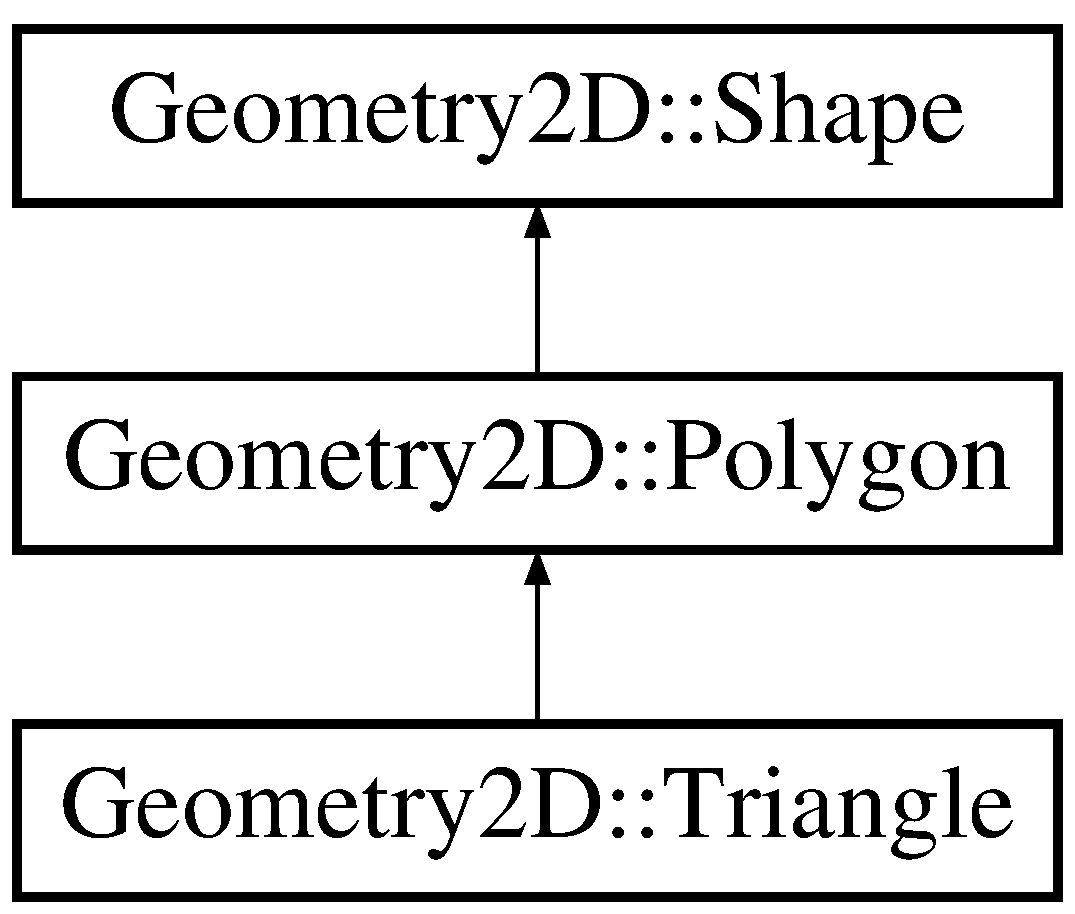
\includegraphics[height=3.000000cm]{class_geometry2_d_1_1_triangle}
\end{center}
\end{figure}
\subsection*{Public Member Functions}
\begin{DoxyCompactItemize}
\item 
\mbox{\hyperlink{class_geometry2_d_1_1_triangle_acd1c0636ad8f7f7659e75a4918770acf}{Triangle}} ()
\item 
\mbox{\Hypertarget{class_geometry2_d_1_1_triangle_a021ed2abfba6fd0683c730c513d80646}\label{class_geometry2_d_1_1_triangle_a021ed2abfba6fd0683c730c513d80646}} 
{\bfseries Triangle} (std\+::vector$<$ cv\+::\+Point $>$ \mbox{\hyperlink{class_geometry2_d_1_1_polygon_ab965e028324c2199022da00ff7eef14b}{points}})
\item 
\mbox{\hyperlink{class_geometry2_d_1_1_triangle_a0b731e9ceb72993005171096adba9096}{$\sim$\+Triangle}} ()
\item 
std\+::vector$<$ cv\+::\+Point $>$ \mbox{\hyperlink{class_geometry2_d_1_1_triangle_af7fa844cf4f260c2c41942e1bffd4c60}{get\+Corners}} ()
\item 
void \mbox{\hyperlink{class_geometry2_d_1_1_triangle_af689573b5d1a3b415ee2c236ed5e3abf}{set\+Corners}} (std\+::vector$<$ cv\+::\+Point $>$ corners)
\item 
\mbox{\Hypertarget{class_geometry2_d_1_1_triangle_aae1d7c21bbade068d34e1dd799e9c742}\label{class_geometry2_d_1_1_triangle_aae1d7c21bbade068d34e1dd799e9c742}} 
void \mbox{\hyperlink{class_geometry2_d_1_1_triangle_aae1d7c21bbade068d34e1dd799e9c742}{assign\+\_\+points}} ()
\begin{DoxyCompactList}\small\item\em assignes points to 1., 2., 3 etc point. \end{DoxyCompactList}\end{DoxyCompactItemize}
\subsection*{Additional Inherited Members}


\subsection{Detailed Description}
class for handling triangle obstacles 

\subsection{Constructor \& Destructor Documentation}
\mbox{\Hypertarget{class_geometry2_d_1_1_triangle_acd1c0636ad8f7f7659e75a4918770acf}\label{class_geometry2_d_1_1_triangle_acd1c0636ad8f7f7659e75a4918770acf}} 
\index{Geometry2\+D\+::\+Triangle@{Geometry2\+D\+::\+Triangle}!Triangle@{Triangle}}
\index{Triangle@{Triangle}!Geometry2\+D\+::\+Triangle@{Geometry2\+D\+::\+Triangle}}
\subsubsection{\texorpdfstring{Triangle()}{Triangle()}}
{\footnotesize\ttfamily Geometry2\+D\+::\+Triangle\+::\+Triangle (\begin{DoxyParamCaption}{ }\end{DoxyParamCaption})}

constructor of triangle class \mbox{\Hypertarget{class_geometry2_d_1_1_triangle_a0b731e9ceb72993005171096adba9096}\label{class_geometry2_d_1_1_triangle_a0b731e9ceb72993005171096adba9096}} 
\index{Geometry2\+D\+::\+Triangle@{Geometry2\+D\+::\+Triangle}!````~Triangle@{$\sim$\+Triangle}}
\index{````~Triangle@{$\sim$\+Triangle}!Geometry2\+D\+::\+Triangle@{Geometry2\+D\+::\+Triangle}}
\subsubsection{\texorpdfstring{$\sim$\+Triangle()}{~Triangle()}}
{\footnotesize\ttfamily Geometry2\+D\+::\+Triangle\+::$\sim$\+Triangle (\begin{DoxyParamCaption}{ }\end{DoxyParamCaption})}

destructor of triangle class 

\subsection{Member Function Documentation}
\mbox{\Hypertarget{class_geometry2_d_1_1_triangle_af7fa844cf4f260c2c41942e1bffd4c60}\label{class_geometry2_d_1_1_triangle_af7fa844cf4f260c2c41942e1bffd4c60}} 
\index{Geometry2\+D\+::\+Triangle@{Geometry2\+D\+::\+Triangle}!get\+Corners@{get\+Corners}}
\index{get\+Corners@{get\+Corners}!Geometry2\+D\+::\+Triangle@{Geometry2\+D\+::\+Triangle}}
\subsubsection{\texorpdfstring{get\+Corners()}{getCorners()}}
{\footnotesize\ttfamily std\+::vector$<$cv\+::\+Point$>$ Geometry2\+D\+::\+Triangle\+::get\+Corners (\begin{DoxyParamCaption}{ }\end{DoxyParamCaption})}

return the list of corners \begin{DoxyReturn}{Returns}
list of corners of the triangle 
\end{DoxyReturn}
\mbox{\Hypertarget{class_geometry2_d_1_1_triangle_af689573b5d1a3b415ee2c236ed5e3abf}\label{class_geometry2_d_1_1_triangle_af689573b5d1a3b415ee2c236ed5e3abf}} 
\index{Geometry2\+D\+::\+Triangle@{Geometry2\+D\+::\+Triangle}!set\+Corners@{set\+Corners}}
\index{set\+Corners@{set\+Corners}!Geometry2\+D\+::\+Triangle@{Geometry2\+D\+::\+Triangle}}
\subsubsection{\texorpdfstring{set\+Corners()}{setCorners()}}
{\footnotesize\ttfamily void Geometry2\+D\+::\+Triangle\+::set\+Corners (\begin{DoxyParamCaption}\item[{std\+::vector$<$ cv\+::\+Point $>$}]{corners }\end{DoxyParamCaption})}

set corners of the triangle 
\begin{DoxyParams}{Parameters}
{\em corners} & list of corners \\
\hline
\end{DoxyParams}


The documentation for this class was generated from the following file\+:\begin{DoxyCompactItemize}
\item 
Triangle.\+hpp\end{DoxyCompactItemize}

\hypertarget{class_image_processing_1_1_undistorsion}{}\section{Image\+Processing\+:\+:Undistorsion Class Reference}
\label{class_image_processing_1_1_undistorsion}\index{Image\+Processing\+::\+Undistorsion@{Image\+Processing\+::\+Undistorsion}}


class for undistorsion of the images  




{\ttfamily \#include $<$Undistortion.\+hpp$>$}

\subsection*{Public Member Functions}
\begin{DoxyCompactItemize}
\item 
\mbox{\hyperlink{class_image_processing_1_1_undistorsion_afeed0c8d0fd647f172a915d44cfb53bf}{Undistorsion}} (std\+::string calibration\+\_\+filename)
\item 
\mbox{\hyperlink{class_image_processing_1_1_undistorsion_a1ce4c30154a1ae1253b8b0d990561ac5}{$\sim$\+Undistorsion}} ()
\item 
void \mbox{\hyperlink{class_image_processing_1_1_undistorsion_ab286d4b5746b8b2716fab24578c27a44}{undistort\+\_\+image}} (cv\+::\+Mat frame, cv\+::\+Mat frame\+Undist, Input\+Array camera\+Matrix, Input\+Array dist\+Coeffs, Input\+Array new\+Camera\+Matrix=no\+Array())
\end{DoxyCompactItemize}


\subsection{Detailed Description}
class for undistorsion of the images 

\subsection{Constructor \& Destructor Documentation}
\mbox{\Hypertarget{class_image_processing_1_1_undistorsion_afeed0c8d0fd647f172a915d44cfb53bf}\label{class_image_processing_1_1_undistorsion_afeed0c8d0fd647f172a915d44cfb53bf}} 
\index{Image\+Processing\+::\+Undistorsion@{Image\+Processing\+::\+Undistorsion}!Undistorsion@{Undistorsion}}
\index{Undistorsion@{Undistorsion}!Image\+Processing\+::\+Undistorsion@{Image\+Processing\+::\+Undistorsion}}
\subsubsection{\texorpdfstring{Undistorsion()}{Undistorsion()}}
{\footnotesize\ttfamily Image\+Processing\+::\+Undistorsion\+::\+Undistorsion (\begin{DoxyParamCaption}\item[{std\+::string}]{calibration\+\_\+filename }\end{DoxyParamCaption})}

construcor of the Undistorion class 
\begin{DoxyParams}{Parameters}
{\em calibration\+\_\+filename} & name of the calibration file \\
\hline
\end{DoxyParams}
\mbox{\Hypertarget{class_image_processing_1_1_undistorsion_a1ce4c30154a1ae1253b8b0d990561ac5}\label{class_image_processing_1_1_undistorsion_a1ce4c30154a1ae1253b8b0d990561ac5}} 
\index{Image\+Processing\+::\+Undistorsion@{Image\+Processing\+::\+Undistorsion}!````~Undistorsion@{$\sim$\+Undistorsion}}
\index{````~Undistorsion@{$\sim$\+Undistorsion}!Image\+Processing\+::\+Undistorsion@{Image\+Processing\+::\+Undistorsion}}
\subsubsection{\texorpdfstring{$\sim$\+Undistorsion()}{~Undistorsion()}}
{\footnotesize\ttfamily Image\+Processing\+::\+Undistorsion\+::$\sim$\+Undistorsion (\begin{DoxyParamCaption}{ }\end{DoxyParamCaption})}

destructor of the Undistortion class 

\subsection{Member Function Documentation}
\mbox{\Hypertarget{class_image_processing_1_1_undistorsion_ab286d4b5746b8b2716fab24578c27a44}\label{class_image_processing_1_1_undistorsion_ab286d4b5746b8b2716fab24578c27a44}} 
\index{Image\+Processing\+::\+Undistorsion@{Image\+Processing\+::\+Undistorsion}!undistort\+\_\+image@{undistort\+\_\+image}}
\index{undistort\+\_\+image@{undistort\+\_\+image}!Image\+Processing\+::\+Undistorsion@{Image\+Processing\+::\+Undistorsion}}
\subsubsection{\texorpdfstring{undistort\+\_\+image()}{undistort\_image()}}
{\footnotesize\ttfamily void Image\+Processing\+::\+Undistorsion\+::undistort\+\_\+image (\begin{DoxyParamCaption}\item[{cv\+::\+Mat}]{frame,  }\item[{cv\+::\+Mat}]{frame\+Undist,  }\item[{Input\+Array}]{camera\+Matrix,  }\item[{Input\+Array}]{dist\+Coeffs,  }\item[{Input\+Array}]{new\+Camera\+Matrix = {\ttfamily noArray()} }\end{DoxyParamCaption})}

function that undistort the image 
\begin{DoxyParams}{Parameters}
{\em frame} & \\
\hline
{\em frame\+Undist} & \\
\hline
{\em camera\+Matrix} & \\
\hline
{\em dist\+Coeffs} & \\
\hline
{\em new\+Camera\+Matrix} & \\
\hline
\end{DoxyParams}


The documentation for this class was generated from the following file\+:\begin{DoxyCompactItemize}
\item 
Undistortion.\+hpp\end{DoxyCompactItemize}

%--- End generated contents ---

% Index
\backmatter
\newpage
\phantomsection
\clearemptydoublepage
\addcontentsline{toc}{chapter}{Index}
\printindex

\end{document}
